% Pengaturan ukuran teks dan bentuk halaman dua sisi
\documentclass[12pt]{report}

% Pengaturan ukuran halaman dan margin
\usepackage[a4paper,top=30mm,left=30mm,right=20mm,bottom=25mm]{geometry}

% Pengaturan ukuran spasi
\usepackage[singlespacing]{setspace}

% Pengaturan caption untuk tabel
\usepackage{caption}

% Judul dokumen
\title{Proposal Tugas Akhir ITS}
\author{Musk, Elon Reeve}

% Pengaturan detail pada file PDF
\usepackage[pdfauthor={\@author},bookmarksnumbered,pdfborder={0 0 0}]{hyperref}


% Pengaturan ukuran indentasi
\setlength{\parindent}{2em}

% Package lainnya
\usepackage{changepage}
\usepackage{etoolbox} % Mengubah fungsi default

% Pengaturan jenis karakter
\usepackage[utf8]{inputenc}

\usepackage[style=apa, backend=biber]{biblatex}
\usepackage{enumitem} % Pembuatan list
\usepackage{lipsum} % Pembuatan template kalimat
\usepackage{graphicx} % Input gambar
\usepackage{longtable} % Pembuatan tabel
\usepackage[table,xcdraw]{xcolor} % Pewarnaan tabel
\usepackage{eso-pic} % Untuk menggunakan background image di halaman
\usepackage{txfonts} % Font times
\usepackage{changepage} % Pembuatan teks kolom
\usepackage{multicol} % Pembuatan kolom ganda
\usepackage{multirow} % Pembuatan baris ganda
\usepackage{tabularx} % Untuk mengatur kolom, seperti grid pada CSS
\usepackage{wrapfig}

% Pengaturan format daftar isi, daftar gambar, dan daftar tabel
\usepackage{tocloft}
\setlength{\cftsecindent}{0cm}
\setlength{\cftsubsecindent}{2em}
\setlength{\cftbeforechapskip}{1.5ex}
\setlength{\cftbeforesecskip}{1.5ex}
\setlength{\cftbeforetoctitleskip}{0cm}
\setlength{\cftbeforeloftitleskip}{0cm}
\setlength{\cftbeforelottitleskip}{0cm}
\renewcommand{\cftsecfont}{\normalfont\bfseries}% membuat judul section pada daftar isi menjadi bold
\renewcommand{\cftsecpagefont}{\normalfont\bfseries}% membuat nomor section daftar isi menjadi bold
\renewcommand{\cfttoctitlefont}{\hfill\Large\bfseries} % command untuk membuat heading bold dan besar
\renewcommand{\cftaftertoctitle}{\hfill}
\renewcommand{\cftloftitlefont}{\hfill\Large\bfseries}
\renewcommand{\cftafterloftitle}{\hfill}
\renewcommand{\cftlottitlefont}{\hfill\Large\bfseries}
\renewcommand{\cftafterlottitle}{\hfill}

% Definisi untuk "Hati ini sengaja dikosongkan"
\patchcmd{\cleardoublepage}{\hbox{}}{
  \thispagestyle{empty}
  \vspace*{\fill}
  \begin{center}\textit{[Halaman ini sengaja dikosongkan]}\end{center}
  \vfill}{}{}

  % Pengaturan penomoran halaman
\usepackage{fancyhdr}
\fancyhf{}
\renewcommand{\headrulewidth}{0pt}
\pagestyle{fancy}
\fancyfoot[C,CO]{\thepage}
\patchcmd{\chapter}{plain}{fancy}{}{}
\patchcmd{\chapter}{empty}{plain}{}{}

% Pengaturan format judul bab
\usepackage{titlesec}
\renewcommand{\thesection}{\arabic{section}}
\titleformat{\chapter}[display]{\bfseries\Large}{BAB \centering\Roman{chapter}}{0ex}{\vspace{0ex}\centering}
\titleformat*{\section}{\large\bfseries}
\titleformat*{\subsection}{\normalsize\bfseries}
\titlespacing{\section}{0ex}{3ex}{1.5ex}
\titlespacing{\subsection}{0ex}{3ex}{1.5ex}
\titlespacing{\subsubsection}{0ex}{0.5ex}{0ex}
\setcounter{secnumdepth}{3} % Untuk memberi penomoran pada \subsubsection

\counterwithin{figure}{section}
\counterwithin{table}{section}

% Mengganti figure dan table menjadi gambar dan tabel
\renewcommand{\figurename}{Gambar}
\renewcommand{\tablename}{Tabel}

% Tambahkan format tanda hubung yang benar di sini
\hyphenation{
  ro-ket
  me-ngem-bang-kan
  per-hi-tu-ngan
}

% Menambahkan resource daftar pustaka
\addbibresource{pustaka/pustaka.bib}

% Isi keseluruhan dokumen
\begin{document}
  % Nomor halaman pembuka dimulai dari sini
  \pagenumbering{roman}

  % Atur ulang penomoran halaman
  \setcounter{page}{1}

  % Sampul Bahasa Indonesia
  \newcommand\covercontents{sampul/konten-id.tex}
  \AddToShipoutPictureBG*{
  \AtPageLowerLeft{
    % Ubah nilai berikut jika posisi horizontal background tidak sesuai
    \hspace{-3.25mm}

    % Ubah nilai berikut jika posisi vertikal background tidak sesuai
    \raisebox{0mm}{
      
\includegraphics[width=\paperwidth,height=\paperheight]{sampul/gambar/sampul-luar.png}
    }
  }
}

% Menyembunyikan nomor halaman
\thispagestyle{empty}

% Pengaturan margin untuk menyesuaikan konten sampul
\newgeometry{
  top=65mm,
  left=30mm,
  right=30mm,
  bottom=20mm
}

\begin{flushleft}

  % Pemilihan font sans serif
  \sffamily

  % Pemilihan font bold
  \fontseries{bx}
  \selectfont
  \begin{spacing}{1.5}
    % Ubah kode buku berikut dengan yang ditentukan oleh departemen
\color{white}
\begin{large}
 TUGAS AKHIR - EC224801
\end{large}

\vspace{\fill}

% Ubah kalimat berikut dengan judul tugas akhir
\begin{spacing}{1.5}
  \begin{Large}
    PREDIKSI HURUF SEMAPHORE BERBASIS POSE MENGGUNAKAN \textit{DEEP LEARNING}% \emph{ANTI-GRAVITASI}
  \end{Large}
\end{spacing}

\vspace{\fill}

% Ubah kalimat-kalimat berikut dengan nama dan NRP mahasiswa
\begin{large}
 Muhammmad Daffa ZW  \\
  \textmd{NRP 0721 19 4000 0064 }
\end{large}

\vspace{\fill}

% Ubah kalimat-kalimat berikut dengan nama-nama dosen pembimbing
\begin{large}
  \textmd{Dosen Pembimbing} \\
   Dr. Eko Mulyanto Yuniarno, S.T., M.T. \\
  \textmd{NIP 19680601199512 1 009} \\
   Ahmad Zaini, S.T., M.T. \\
  \textmd{NIP: 19750419200212 1 003 }
\end{large}

\vspace{\fill}

% Ubah kalimat-kalimat berikut dengan nama departemen dan fakultas
Program Studi Strata 1 (S1) Teknik Komputer \\

\mdseries

Departemen Teknik Komputer \\
Fakultas Teknologi Elektro dan Informatika Cerdas \\
Institut Teknologi Sepuluh Nopember

% Ubah kalimat berikut dengan tempat dan tahun pembuatan buku
Surabaya \\
2023

  \end{spacing}

\end{flushleft}

\restoregeometry


  % Sampul Bahasa Inggris
  \renewcommand\covercontents{sampul/konten-en.tex}
  \AddToShipoutPictureBG*{
  \AtPageLowerLeft{
    % Ubah nilai berikut jika posisi horizontal background tidak sesuai
    \hspace{-3.25mm}

    % Ubah nilai berikut jika posisi vertikal background tidak sesuai
    \raisebox{0mm}{
      
\includegraphics[width=\paperwidth,height=\paperheight]{sampul/gambar/sampul-luar.png}
    }
  }
}

% Menyembunyikan nomor halaman
\thispagestyle{empty}

% Pengaturan margin untuk menyesuaikan konten sampul
\newgeometry{
  top=65mm,
  left=30mm,
  right=30mm,
  bottom=20mm
}

\begin{flushleft}

  % Pemilihan font sans serif
  \sffamily

  % Pemilihan font bold
  \fontseries{bx}
  \selectfont
  \begin{spacing}{1.5}
    % Ubah kode buku berikut dengan yang ditentukan oleh departemen
\color{white}
\begin{large}
 TUGAS AKHIR - EC224801
\end{large}

\vspace{\fill}

% Ubah kalimat berikut dengan judul tugas akhir
\begin{spacing}{1.5}
  \begin{Large}
    PREDIKSI HURUF SEMAPHORE BERBASIS POSE MENGGUNAKAN \textit{DEEP LEARNING}% \emph{ANTI-GRAVITASI}
  \end{Large}
\end{spacing}

\vspace{\fill}

% Ubah kalimat-kalimat berikut dengan nama dan NRP mahasiswa
\begin{large}
 Muhammmad Daffa ZW  \\
  \textmd{NRP 0721 19 4000 0064 }
\end{large}

\vspace{\fill}

% Ubah kalimat-kalimat berikut dengan nama-nama dosen pembimbing
\begin{large}
  \textmd{Dosen Pembimbing} \\
   Dr. Eko Mulyanto Yuniarno, S.T., M.T. \\
  \textmd{NIP 19680601199512 1 009} \\
   Ahmad Zaini, S.T., M.T. \\
  \textmd{NIP: 19750419200212 1 003 }
\end{large}

\vspace{\fill}

% Ubah kalimat-kalimat berikut dengan nama departemen dan fakultas
Program Studi Strata 1 (S1) Teknik Komputer \\

\mdseries

Departemen Teknik Komputer \\
Fakultas Teknologi Elektro dan Informatika Cerdas \\
Institut Teknologi Sepuluh Nopember

% Ubah kalimat berikut dengan tempat dan tahun pembuatan buku
Surabaya \\
2023

  \end{spacing}

\end{flushleft}

\restoregeometry


  % Lembar pengesahan
  \chapter*{LEMBAR PENGESAHAN}

% Menyembunyikan nomor halaman
\thispagestyle{empty}

\begin{center}
  % Ubah kalimat berikut dengan judul tugas akhir
  \textbf{PREDIKSI HURUF SEMAPHORE BERBASIS POSE MENGGUNAKAN \emph{DEEP LEARNING}}
\end{center}

\begingroup
% Pemilihan font ukuran small
\small

\begin{center}
  % Ubah kalimat berikut dengan pernyataan untuk lembar pengesahan
  \textbf{PROPOSAL TUGAS AKHIR} \\
  Diajukan untuk memenuhi salah satu syarat memperoleh gelar
  Sarjana Teknik pada
  Program Studi S-1 Teknik Komputer \\
  Departemen Teknik Komputer \\
  Fakultas Teknologi Elektro  dan Informatika Cerdas \\
  Institut Teknologi Sepuluh Nopember
\end{center}

\begin{center}
  % Ubah kalimat berikut dengan nama dan NRP mahasiswa
  Oleh: \textbf{Muhammad Daffa ZW} \\
  NRP. 0721 19 4000 0064
\end{center}

\begin{center}
  Disetujui Oleh:
\end{center}

\vspace{10ex}

\begingroup
% Menghilangkan padding
\setlength{\tabcolsep}{0pt}

\noindent
\begin{tabularx}{\textwidth}{X c}
  % Ubah kalimat-kalimat berikut dengan nama dan NIP dosen pembimbing pertama
  Dr Eko Mulyanto Yuniarno , S.T , M.T.      &                 \\
  NIP: 196806011995121009   & (Pembimbing)    \\
  & ................................... \\
  &  \\
  &  \\
  % Ubah kalimat-kalimat berikut dengan nama dan NIP dosen pembimbing kedua
  Ahmad Zaini, S.T., M.T. &                 \\
  NIP: 197504192002121003   & (Ko-Pembimbing) \\
  & ................................... \\
  &  \\
  &  \\
  Dr. Diah Puspito Wulandari, S.T., M.Sc.    &                 \\
  NIP: 198012192005012001   & (Penguji I)    \\
  & ................................... \\
  &  \\
  &  \\
  % Ubah kalimat-kalimat berikut dengan nama dan NIP dosen pembimbing kedua
  Reza Fuad Rachmadi, S.T., M.T., Ph.D  &                 \\
  NIP: 198504032012121001   & (Penguji II) \\
  & ................................... \\
  &  \\
  &  \\
\end{tabularx}
\endgroup


\begin{center}
  % Ubah kalimat berikut dengan jabatan kepala departemen
  Mengetahui, \\
  Kepala Departemen Teknik Komputer FTEIC - ITS\\

  \vspace{8ex}

  % Ubah kalimat-kalimat berikut dengan nama dan NIP kepala departemen
  \underline{Dr. Supeno Mardi Susiki Nugroho, S.T., M.T.} \\
  NIP. 19700313 199512 1 000
\end{center}
  
\begin{center}
  \textbf{SURABAYA\\Juli, 2023}
\end{center}
\endgroup

  \newpage

  % Lembar pengesahan
  \begin{center}
	\large
  \textbf{APPROVAL SHEET}
\end{center}

% Menyembunyikan nomor halaman
\thispagestyle{empty}

\begin{center}
  % Ubah kalimat berikut dengan judul tugas akhir
  \textbf{POSE BASED SEMAPHORE PREDICTION USING DEEP LEARNING}
\end{center}

\begingroup
  % Pemilihan font ukuran small
  \small

  \begin{center}
    % Ubah kalimat berikut dengan pernyataan untuk lembar pengesahan
    \textbf{FINAL PROJECT PROPOSAL} \\
    Submitted to fulfill one of the requirements for obtaining a degree
    Bachelor of Engineering at 
    Undergraduate Study Program of Computer Engineering \\
    Department of Computer Engineering \\
    FacultyOf Intelligent Electrical and Informatics Technology  \\
    Sepuluh Nopember Institute of Technology
  \end{center}

  \begin{center}
    % Ubah kalimat berikut dengan nama dan NRP mahasiswa
    By: \textbf{Muhammad Daffa ZW} \\
    NRP. 0721 19 4000 0064
  \end{center}

  \begin{center}
    Approved by Final Project Proposal Examiner Team:
  \end{center}

  \begingroup
    % Menghilangkan padding
    \setlength{\tabcolsep}{0pt}

    \noindent
    \begin{tabularx}{\textwidth}{X c}                        
      % Ubah kalimat-kalimat berikut dengan nama dan NIP dosen pembimbing pertama
      Dr Eko Mulyanto Yuniarno , S.T , M.T.       & (Advisor) \\
      NIP: 196806011995121009      & \\
      & ................................... \\
      &  \\
      &  \\
      % Ubah kalimat-kalimat berikut dengan nama dan NIP dosen pembimbing kedua
      Ahmad Zaini, S.T., M.T.     & (Co-Advisor) \\
      NIP: 197504192002121003        & \\
      & ................................... \\
      &  \\
      &  \\
      Dr. Diah Puspito Wulandari, S.T., M.Sc.    &                 \\
      NIP: 198012192005012001   & (Examiner I)    \\
      & ................................... \\
      &  \\
      &  \\            
      % Ubah kalimat-kalimat berikut dengan nama dan NIP dosen pembimbing kedua
      Reza Fuad Rachmadi, S.T., M.T., Ph.D &                 \\
      NIP: 198504032012121001   & (Examiner II) \\
      & ................................... \\
      &  \\
      &  \\   
    \end{tabularx}
  \endgroup

  \begin{center}
    % Ubah kalimat berikut dengan jabatan kepala departemen
    Acknowledged, \\
    Head of Computer Engineering Department\\

    \vspace{8ex}

    % Ubah kalimat-kalimat berikut dengan nama dan NIP kepala departemen
    \underline{Dr. Supeno Mardi Susiki Nugroho, S.T., M.T.} \\
    NIP. 19700313 199512 1 000
  \end{center}

  \begin{center}
    \textbf{SURABAYA\\July, 2023}
  \end{center}
\endgroup
  \newpage

  % Abstrak
  \chapter*{ABSTRAK}
\begin{center}
  \large
  \textbf{POSE BASED SEMAPHORE PREDICTION USING DEEP LEARNING \emph{DEEP LEARNING}}
\end{center}
\addcontentsline{toc}{chapter}{ABSTRAK}
% Menyembunyikan nomor halaman
\thispagestyle{empty}

\begin{flushleft}
  \setlength{\tabcolsep}{0pt}
  \bfseries
  \begin{tabular}{ll@{\hspace{6pt}}l}
  Nama Mahasiswa / NRP&:& Muhammad Daffa ZW / 0721 19 4000 0064\\
  Departemen&:& Teknik Komputer - FTEIC - ITS \\
  Dosen Pembimbing&:& 1. Dr Eko Mulyanto Yuniarno , S.T , M.T.\\
  & & 2. Ahmad Zaini, S.T., M.T.\\
  \end{tabular}
  \vspace{4ex}
\end{flushleft}
\textbf{Abstrak}

% Isi Abstrak
Penelitian ini bertujuan untuk mengembangkan sistem prediksi huruf semaphore menggunakan teknologi deep learning dengan implementasi convolutional neural network (CNN). Batasan masalah dari penelitian ini adalah hanya huruf alfabet yang dapat dideteksi menggunakan pose tubuh, dan metode deep learning yang diaplikasikan adalah CNN. Tujuan dari penelitian ini adalah untuk menerapkan deteksi pose manusia menggunakan MediaPipe kepada tangan, menerjemahkan gestur semaphore pramuka menjadi audio Bahasa Indonesia, serta memberikan pengalaman pembelajaran interaktif tentang semaphore. Penelitian ini diharapkan dapat membantu dan memudahkan dalam mempelajari bendera semaphore, meskipun penggunaannya saat ini telah berkurang.

\vspace{2ex}
\noindent
\textbf{Kata Kunci: \emph{Bendera Semaphore, Deep Learning, Convolutional Neural Network, Estimasi Pose Tubuh Manusia, MediaPipe, Pembelajaran Interaktif.}}
  \newpage

  \chapter*{ABSTRACT}
\begin{center}
  \large
  \textbf{    \emph{POSE BASED} SEMAPHORE PREDICTION USING DEEP LEARNING }
\end{center}
% Menyembunyikan nomor halaman
\thispagestyle{empty}

\begin{flushleft}
  \setlength{\tabcolsep}{0pt}
  \bfseries
  \begin{tabular}{lc@{\hspace{6pt}}l}
  Student Name / NRP&: &Muhammmad Daffa ZW / 07211940000064\\
  Department&: &Computer Engineering FTEIC - ITS\\
  Advisor&: &1. Dr. Eko Mulyanto Yuniarno, S.T., M.T.\\
  & & 2.  Ahmad Zaini, S.T., M.T.\\
  \end{tabular}
  \vspace{4ex}
\end{flushleft}
\textbf{Abstract}

% Isi Abstrak
The visual communication system using semaphore has been widely used in various fields such as the military, maritime, and transportation sectors. This method involves the use of flags or hand signals to transmit messages between two or more parties. However, traditional semaphore usage requires special training, expertise, and the ability to understand complex semaphore codes.This research aims to develop a semaphore pose recognition system using MediaPipe and Deep Learning classification through Convolutional Neural Network (CNN) methods. The development process involves steps such as dataset collection and processing, pose extraction using MediaPipe, and pose classification using CNN models such as CNN, CNN ResNet50V2, and CNN Xception.The results of this research demonstrate that the developed system is capable of accurately detecting letters and words in semaphore poses. The CNN ResNet50V2 model achieved an accuracy of 98.08\%, CNN Xception achieved 98.78\%, CNN achieved 98.94\%, and CNN2 achieved 99.1\%. Based on these findings, the semaphore pose recognition system has potential applications in education, particularly in schools. With the help of this technology, learning about semaphore can become more engaging and interactive. Students can learn visual communication through semaphore with the assistance of a system that can detect and recognize letter and word poses. The use of the semaphore pose recognition system in education also opens up possibilities for further exploration in the development of other interactive learning methods.


\vspace{2ex}
\noindent
\textbf{Keywords: \emph{Semaphore, MediaPipe, Convolutional Neural Network , Human Pose, Deep Learning , Xception , ResNet50V2 }}
  \newpage

  \begin{spacing}{1.5}
    % Daftar isi
    \renewcommand*\contentsname{DAFTAR ISI}
    \addcontentsline{toc}{chapter}{\contentsname}
    \tableofcontents
    \newpage

    % Daftar gambar
    \renewcommand*\listfigurename{DAFTAR GAMBAR}
    \addcontentsline{toc}{chapter}{\listfigurename}
    \listoffigures
    \newpage

    % Daftar tabel
    \renewcommand*\listtablename{DAFTAR TABEL}
    \addcontentsline{toc}{chapter}{\listtablename}
    \listoftables
    \newpage
  \end{spacing}

  % Nomor halaman isi dimulai dari sini
  \pagenumbering{arabic}

  % Konten pendahuluan
  \section{PENDAHULUAN}

\subsection{Latar Belakang}

% Ubah paragraf-paragraf berikut sesuai dengan latar belakang dari tugas akhir
Pramuka merupakan singkatan dari Praja Muda Karana yang berbentuk dalam sebuah Organisasi atau Gerakan Kepanduan yang di Indonesia sendiri biasa disebut dengan Gerakan Pramuka . Di Dalam Dunia Internasional dikenal dengan nama Kepanduan atau biasa disebut Boy Scout . Gerakan Pramuka memiliki Kode Kehormatan yang terdiri dari janji yang disebut dengan Satya dan Ketentuan Moral . Pramuka sendiri dibagi menjadi beberapa golongan yaitu Siaga , Penggalang , Penegak dan Pandega 
 

 Semaphore merupakan sebuah cara berkomunikasi satu dengan lainnya yang saling berjauhan dengan dua tangan memegang bendara . Dari pose yang diperagakan maka bisa diterima informasi tentang huruf apa yang diperagakan . Semaphore merupakan materi yang diajarkan didalam materi Pramuka di setiap sekolah-sekolah . Manfaat mempelajari semaphore sendiri adalah agar setiap anggota Pramuka bisa berkomunikasi satu sama lain di situasi susah sinyal 

 Permasalahan yang dihadapi dalam Semaphore dalam Dunia Pendidikan sendiri adalah masih banyak anak-anak yang kesulitan dalam memahami Gerakan-gerakan semaphore dalam pembelajaran Pramuka , Penelitian tentang pemanfaatan teknologi visi computer yaitu tensor flow dalam sistem deteksi tubuh manusia


\subsection{Rumusan Masalah}

% Ubah paragraf berikut sesuai dengan rumusan masalah dari tugas akhir
Saat ini sedikit sekali orang yang bisa menguasai dan membaca huruf semaphore , Oleh karena itu diperlukan sebuah Teknologi yang dapat membantu untuk menyelesaikan persoalan ini yaitu dengan cara menggunakan pendekatan Deep Learning 


\subsection{Batasan Masalah atau Ruang Lingkup}

Berdasarkan dari tujuan penelitian ini, diperlukan adanya batasan-batasan masalah untuk memperjelas cakupan dari penelitian yang dilakukan. Adapun batasan-batasan tersebut sebagai berikut:

\begin{enumerate}
\item Huruf Yang Dideteksi Sebanyak 10 Huruf
\item Huruf Yang Dideteksi Adalah Huruf Alphabet 
\end{enumerate}


\subsection{Tujuan}


% Ubah paragraf berikut sesuai dengan tujuan penelitian dari tugas akhir


Tujuan dari penelitian ini adalah :

\begin{enumerate}   
\item	Menerapkan deteksi pose manusia menggunakan MediaPipe kepada tangan
\item	Menerjemahkan gestur semaphore pramuka menjadi audio Bahasa Indonesia
\item	Memberikan pengalaman pembelajaran interaktif tentang semaphore
\end{enumerate}


\subsection{Manfaat}

% Ubah paragraf berikut sesuai dengan tujuan penelitian dari tugas akhir
Manfaat dari penelitian ini adalah : 

\begin{enumerate}  
\item	Bagi penulis manfaat yang akan didapat adalah menambah ilmu dalam visi komputer dan Deep Learning dalam penggunaan MediaPipe.
\item	Bagi Institusi manfaat yang akan didapat adalah bentuk pengimplementasian yang nyata terhadap ilmu visi komputer.
\item	Bagi peneliti manfaat yang didapat adalah dapat mengembangkan model machine learning dengan menggunakan MediaPipe dan juga model Deep Learning.
\item	Bagi Siswa yang masih sekolah bisa bermanfaat untuk membantu dalam proses pembelajaran semaphore yang dilaksanakan didalam kegiatan pramuka
\end{enumerate}



  % Konten tinjauan pustaka
  \chapter{TINJAUAN PUSTAKA}

% Ubah konten-konten berikut sesuai dengan isi dari tinjauan pustaka
\section{Hasil Penelitian Terdahulu}
Pada penelitian sebelumnya telah dilakukan dalam rangka menginvestigasi implementasi deteksi objek secara \textit{real time} berbasis \textit{YOLO (You Only Look Once)} \cite{redmon2016you}. Selain itu, terdapat juga penelitian yang memfokuskan pada pengembangan metode deteksi postur yoga menggunakan platform \textit{MediaPipe} \cite{garg2022yoga}. Penelitian selanjutnya telah membahas tentang penggunaan \textit{MediaPipe} dan \textit{Machine Learning} dalam mendeteksi posisi bagi keperluan pelatihan \cite{supanich2023machine}. Sebuah studi lainnya telah mengkaji penggunaan \textit{MediaPipe} dalam memonitor latihan bicep curl dengan tujuan penguatan otot \cite{nguyen2023assessing}. Selanjutnya, dalam konteks yang berbeda, terdapat penelitian yang melibatkan penggunaan model \textit{Faster-RCNN-Inception-V2-COCO} dari \textit{TensorFlow} dalam melakukan pengenalan gestur semaphore menggunakan bendera \cite{motty2023flag}. Metode ini memanfaatkan \textit{TensorFlow API} dan Model \textit{Deep Neural Network (DNN)} dalam melatih model dan melakukan deteksi gestur semaphore.

Pada penelitian-penelitian tersebut, pendekatan pasif digunakan dalam menganalisis dan mengidentifikasi objek, postur yoga, posisi pelatihan, serta gestur semaphore. Melalui penggunaan teknologi yang canggih, seperti \textit{YOLO}, \textit{MediaPipe}, \textit{Machine Learning}, dan model \textit{Deep Neural Network (DNN)}, para peneliti telah mampu mencapai deteksi yang efisien dan akurat. Penelitian-penelitian ini berkontribusi dalam memperluas pemahaman dan penerapan teknologi dalam berbagai bidang, mulai dari deteksi objek hingga pengenalan gestur semaphore dengan bantuan komputasi yang kuat.

\section{Bendera Semaphore}
\begin{figure}[hbt!]
  \centering
	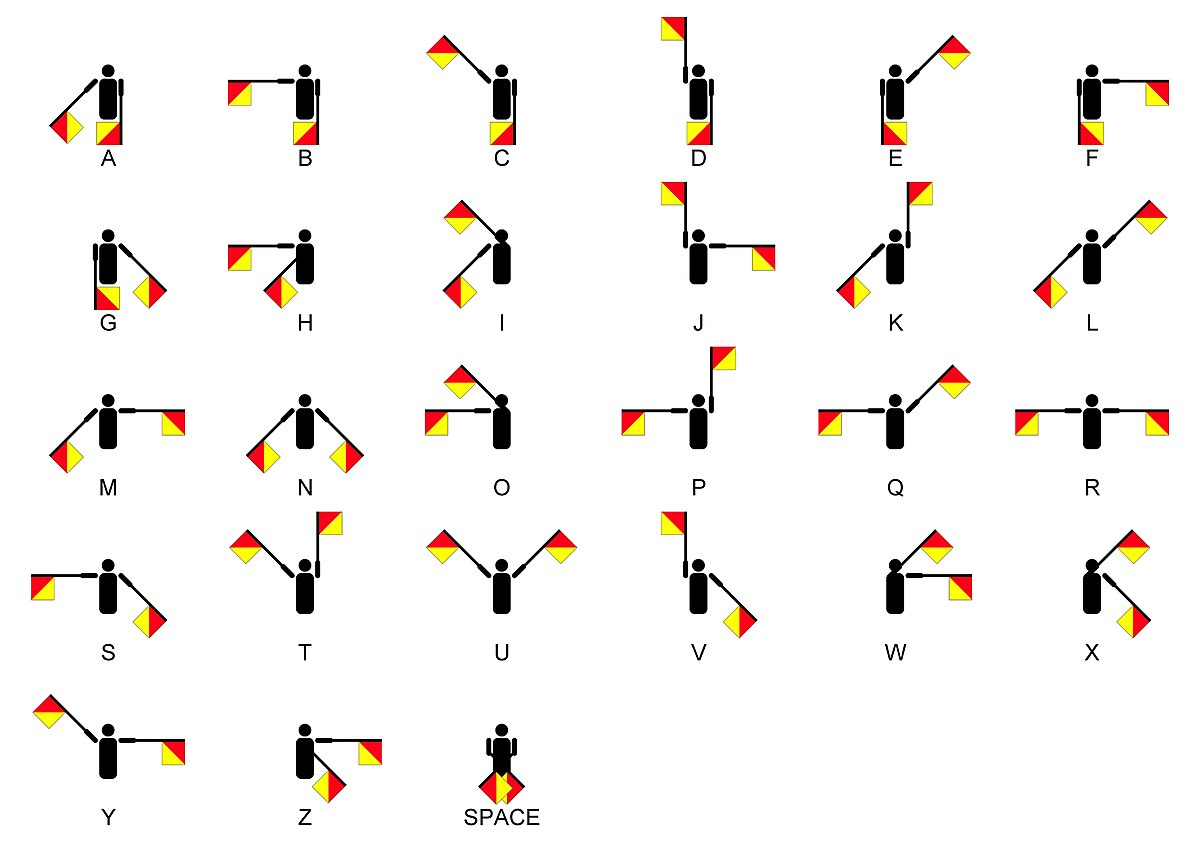
\includegraphics[width=0.7\linewidth]{gambar/bener/Semaphore-Pose.jpg}
	\captionof{figure}{Bendera Semaphore}
	\label{fig:BenderaSemaphore}
\end{figure}

Bendera Semaphore adalah sebuah sistem komunikasi yang dikembangkan pada abad ke-18 oleh Claude Chappe, seorang ahli matematika Prancis, sebagai cara mengirim pesan telegraf tanpa menggunakan kabel \cite{8752707}. Dalam sistem ini, dua bendera yang dapat digerakkan ke posisi yang berbeda digunakan dalam mewakili huruf dan angka dalam alfabet seperti \ref{fig:BenderaSemaphore}. Melalui pengaturan posisi bendera-bendera tersebut, pesan dapat ditransmisikan kepada penerima pesan tanpa memerlukan infrastruktur kabel yang rumit. Bendera Semaphore umumnya digunakan dalam situasi di mana komunikasi jarak jauh diperlukan, seperti antara kapal atau kota-kota yang terpisah \cite{gundogdu2019semaphore}.

Penggunaan sistem komunikasi bendera Semaphore membawa manfaat yang signifikan pada masa ketika teknologi komunikasi belum mencapai tingkat kemajuan seperti sekarang. Pesan dapat dikirim dengan cepat dan efisien tanpa ketergantungan pada koneksi kabel yang terbatas pada waktu itu. Dalam era tersebut, peran sistem ini dalam meningkatkan efektivitas dan kecepatan pertukaran informasi antarlokasi yang terpisah tidak dapat diabaikan. Komunikasi jarak jauh menjadi lebih efisien dan andal berkat sistem bendera Semaphore yang ditemukan oleh Claude Chappe pada abad ke-18. Dengan demikian, dapat disimpulkan bahwa bendera Semaphore merupakan sebuah sistem komunikasi yang menggunakan dua bendera yang dapat diposisikan ke berbagai posisi agar bisa mengirimkan pesan jarak jauh. Sistem ini ditemukan oleh Claude Chappe pada abad ke-18 sebagai solusi mengatasi keterbatasan koneksi kabel pada masa itu. Pemanfaatan bendera Semaphore membawa manfaat yang signifikan dalam meningkatkan efisiensi dan keandalan komunikasi jarak jauh pada era tersebut.

\section{Estimasi Pose}
Estimasi pose adalah suatu teknik atau metode yang sangat relevan dan berharga dalam berbagai bidang aplikasi, seperti augmented reality, robotika, pemrosesan citra, dan pengenalan gerakan. Kemampuan memperkirakan dengan tepat posisi dan orientasi objek dalam ruang tiga dimensi memungkinkan pengembangan solusi yang lebih canggih dan tepat dalam berbagai konteks.Dalam konteks penggunaan kamera, estimasi pose menjadi semakin penting karena berbagai kemajuan dalam teknologi kamera dan sensor, termasuk sensor kamera dengan resolusi tinggi, kamera multi-view, dan bahkan kamera yang terintegrasi dengan sensor kedalaman. Keberadaan data sensor yang kaya memberikan potensi besar  meningkatkan akurasi dan ketepatan estimasi pose.

Proses estimasi pose bisa menjadi tantangan tersendiri karena melibatkan beberapa langkah kompleks. Pertama-tama, data sensor yang relevan harus dikumpulkan dengan hati-hati, dan hal ini dapat melibatkan pengaturan kamera yang tepat, kalibrasi, dan penyesuaian parameter sensor lainnya. Selanjutnya, langkah kritis berikutnya adalah mengidentifikasi fitur-fitur penting dalam data sensor yang didapatkan, seperti menemukan titik-titik referensi, tepi, atau fitur-fitur geometris lainnya. Pemilihan fitur yang tepat dan akurat adalah kunci utama kesuksesan dalam estimasi pose. Setelah fitur-fitur relevan diidentifikasi, langkah selanjutnya adalah mencocokkan atau membandingkan fitur-fitur tersebut dengan fitur-fitur yang diketahui atau telah direkam sebelumnya. Metode pencocokan ini dapat sangat bervariasi, dan tergantung pada jenis data sensor yang digunakan dan konteks aplikasi. Dalam beberapa kasus, estimasi pose juga melibatkan pencocokan dengan model geometris atau model 3D objek yang diketahui, yang memerlukan komputasi yang lebih rumit dan penggunaan algoritma yang lebih canggih.  \cite{Andriluka_2014_CVPR}

Di era modern ini, terutama dengan perkembangan pesat dalam bidang kecerdasan buatan, teknik estimasi pose semakin dipengaruhi oleh pendekatan berbasis \textit{Deep Learning}. Penggunaan jaringan saraf tiruan dan model \textit{deep neural network} telah membuktikan kehebatannya dalam memahami fitur-fitur kompleks dalam data sensor dan menghasilkan estimasi pose yang lebih akurat dan dapat diandalkan. Namun, kendati perkembangan teknologi yang pesat, tantangan dalam estimasi pose masih ada, terutama ketika menghadapi situasi yang kompleks dan tidak terstruktur. Selain itu, faktor lingkungan seperti pencahayaan, bayangan, dan perubahan kondisi sekitar juga dapat mempengaruhi kualitas estimasi pose. Oleh karena itu, para peneliti terus bekerja meningkatkan teknik estimasi pose dengan menggabungkan pendekatan-pendekatan yang berbeda, mengoptimalkan algoritma yang ada, dan menggunakan data sensor yang semakin canggih.

Dalam beberapa tahun terakhir, metode estimasi pose telah menjadi fokus utama dalam penelitian dan pengembangan di berbagai industri. Penggunaan augmented reality dalam permainan dan aplikasi lainnya semakin menuntut akurasi estimasi pose yang lebih tinggi. Di bidang robotika, kemampuan robot mengenali dan memahami posisi objek di sekitarnya sangat penting bagi keberhasilan tugas yang rumit dan kompleks. Bahkan dalam pemrosesan citra dan pengenalan gerakan, estimasi pose berperan penting dalam analisis dan pengolahan data. \cite{Toshev_2014_CVPR} . Secara keseluruhan, estimasi pose adalah bidang yang menarik dan penting, dengan aplikasi yang meluas dan beragam. Dengan terus majunya teknologi sensor dan perkembangan dalam bidang kecerdasan buatan, diharapkan estimasi pose akan terus berkembang dan memberikan kontribusi yang signifikan dalam berbagai industri dan aplikasi kehidupan sehari-hari.

\section{MediaPipe}
\textit{MediaPipe} merupakan sebuah \textit{framework} yang sangat fleksibel dan efisien dalam mengelola dan memproses input sensori seperti video dan audio. Dikembangkan oleh tim \textit{Google Research}, \textit{MediaPipe} menyediakan beragam komponen persepsi yang dapat digabungkan dengan mudah dalam membuat prototipe dan mengembangkan aplikasi canggih yang dapat dijalankan di berbagai platform. Keunggulan \textit{MediaPipe} terletak pada kemampuannya mengoptimalkan penggunaan sumber daya dengan mengurangi latensi, menangani sinkronisasi data seri waktu, serta melakukan pengukuran kinerja dan konsumsi sumber daya. Dengan performa yang baik dan efisiensi dalam pemrosesan input sensori, \textit{MediaPipe} menjadi pilihan yang menarik bagi para pengembang aplikasi. Salah satu komponen unggulan dalam \textit{MediaPipe} adalah Estimasi Posisi Manusia (\textit{Human Pose Estimation}). Estimasi Pose Manusia merupakan teknik yang bertujuan mendeteksi dan mengidentifikasi posisi tubuh manusia dalam gambar atau video. Dengan menggunakan algoritma dan model yang ada dalam \textit{MediaPipe}, pengembang dapat dengan mudah mengintegrasikan kemampuan ini ke dalam aplikasi mereka. Estimasi Pose Manusia memungkinkan analisis lanjutan terhadap posisi tubuh manusia dalam video atau gambar, membuka peluang mengembangkan berbagai aplikasi yang melibatkan interaksi manusia. \cite{lugaresi2019mediapipe}
\begin{figure}[hbt!]
  \centering
  % Nama dari file gambar yang diinputkan
  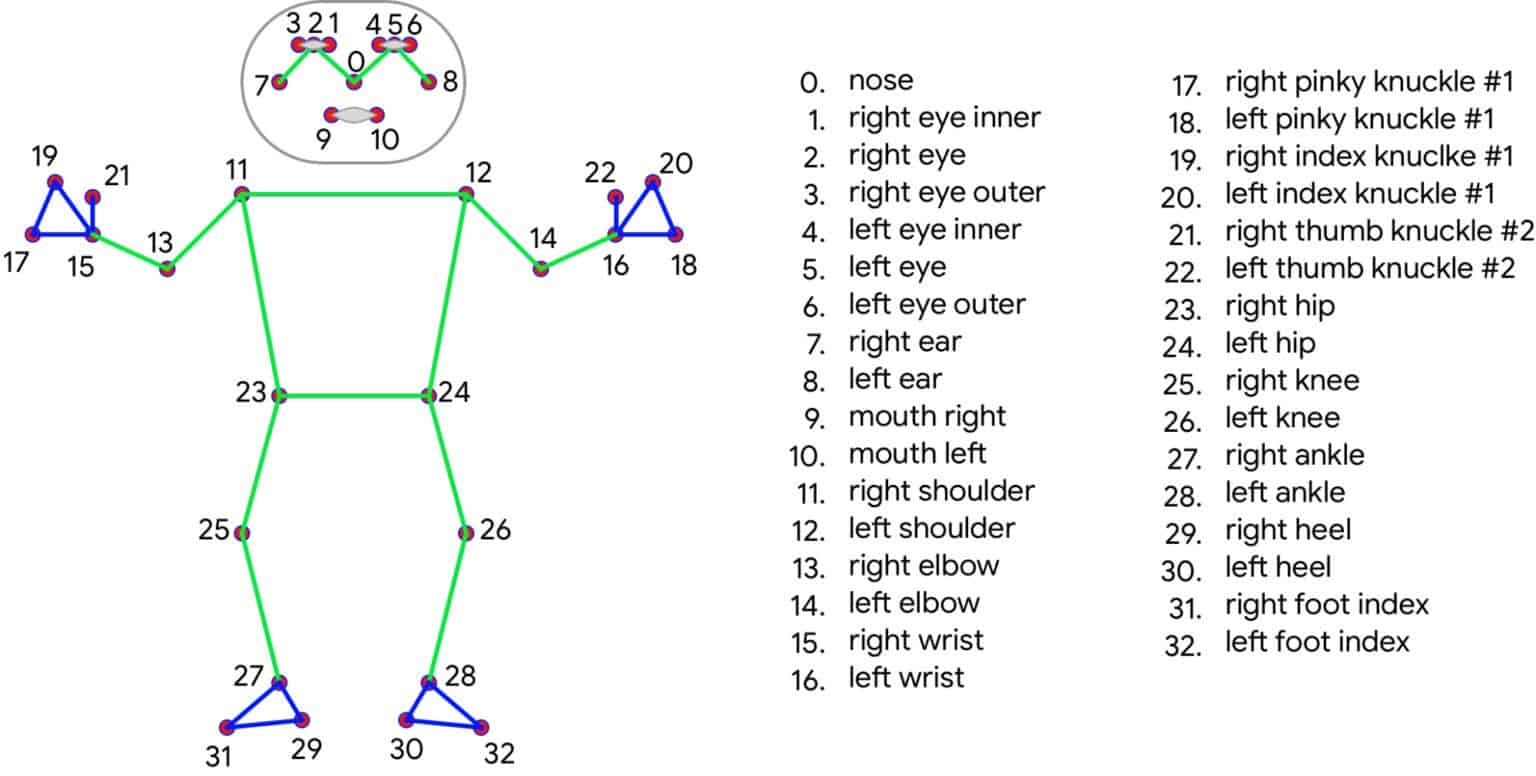
\includegraphics[width=0.7\linewidth]{gambar/humanpose.jpg}
  % Keterangan gambar yang diinputkan
  \captionof{figure}{Human Pose Skeleton MediaPipe}
  % Label referensi dari gambar yang diinputkan
  \label{fig:Pose Tubuh dari MediaPipe}
\end{figure}
Sebagai contoh, dengan memanfaatkan Estimasi Pose Manusia dari \textit{MediaPipe} seperti pada Gambar \ref{fig:Pose Tubuh dari MediaPipe} , pengembang dapat menciptakan aplikasi deteksi gerakan yang mengenali gerakan tubuh pengguna untuk mengendalikan perangkat atau berinteraksi dengan aplikasi secara intuitif. Aplikasi semacam ini sangat relevan dalam industri game dan realitas virtual, di mana interaksi alami dan lancar dengan dunia virtual menjadi sangat diinginkan. Selain itu, Estimasi Pose Manusia juga memungkinkan pengenalan gestur tubuh, di mana aplikasi dapat mengenali dan menafsirkan gerakan tangan atau tubuh pengguna sebagai perintah atau kontrol khusus. Contohnya adalah dalam pengembangan aplikasi \textit{sign language recognition} yang dapat menerjemahkan gerakan bahasa isyarat menjadi teks atau ucapan, membantu komunikasi bagi orang-orang dengan gangguan pendengaran. \cite{singh2021real}

Fitur Estimasi Pose Manusia juga dapat dimanfaatkan dalam bidang olahraga dan rehabilitasi fisik. Dalam olahraga, aplikasi dapat mengukur dan menganalisis postur tubuh atlet memberikan umpan balik dan perbaikan teknik. Sedangkan dalam rehabilitasi fisik, aplikasi dapat membantu pasien mengikuti latihan fisioterapi dengan benar dengan mengenali postur tubuh mereka dan memberikan petunjuk visual atau suara.Dalam lingkungan penelitian, Estimasi Pose Manusia dapat digunakan dalam analisis gerakan manusia, seperti dalam studi biomekanika, pengenalan tindakan manusia, atau pengamatan perilaku manusia. Data posisi tubuh manusia yang akurat dan real-time yang diberikan oleh \textit{MediaPipe} mempermudah peneliti melakukan analisis yang mendalam terhadap berbagai aspek gerakan manusia. Salah satu konsep yang mendukung kemampuan Estimasi Pose Manusia dalam \textit{MediaPipe} adalah \textit{Human Pose Skeleton} (\textit{kerangka tubuh manusia}). \textit{MediaPipe} menghasilkan representasi kerangka tubuh manusia dalam bentuk \textit{skeleton} yang terdiri dari serangkaian titik-titik kunci (\textit{keypoints}) yang menggambarkan posisi sendi-sendi dan bagian tubuh manusia. Informasi tentang posisi sendi-sendi ini memberikan gambaran yang sangat berguna tentang postur dan gerakan tubuh manusia dalam video atau gambar. 

Titik-titik \textit{landmark} tersebut terdiri dari berbagai bagian tubuh, seperti kepala, leher, bahu, siku, pergelangan tangan, panggul, lutut, hingga pergelangan kaki. Total jumlah \textit{landmark} yang digunakan dalam Mediapipe adalah 33 titik. Setiap titik \textit{landmark} ini memiliki koordinat yang menunjukkan posisi relatif terhadap citra atau frame video yang sedang dianalisis. Dengan informasi titik-titik \textit{landmark} ini, Mediapipe dapat mengkonstruksi pose skeleton dengan menghubungkan titik-titik tersebut sesuai dengan struktur anatomi tubuh manusia. Hasil dari pendeteksian pose skeleton ini dapat digunakan dalam berbagai tujuan, seperti analisis gerakan tubuh, klasifikasi aktivitas manusia, pembuatan animasi, dan pengenalan gerakan.

\textit{MediaPipe} menyediakan \textit{skeleton} dengan akurasi tinggi dan kemampuan pelacakan yang andal. Selain itu, \textit{skeleton} tersebut dapat diintegrasikan dengan mudah ke dalam aplikasi lain atau digunakan sebagai input berbagai tugas analisis dan pengenalan gerakan. Representasi \textit{skeleton} ini memberikan representasi yang ringkas namun informatif tentang tubuh manusia, sehingga memudahkan pengembang dan peneliti bekerja dengan data pose manusia.Secara keseluruhan, Fitur Estimasi Pose Manusia yang berasal dari \textit{Human Pose Skeleton} , Fitur \textit{MediaPipe} adalah fitur yang kuat dan berguna dalam mengolah input sensori berupa video dan gambar. Dengan kemampuan ini, \textit{MediaPipe} membuka peluang yang luas bagi pengembangan aplikasi interaktif, analisis gerakan, pengenalan gestur, hingga aplikasi di bidang olahraga dan rehabilitasi fisik. Kecepatan dan efisiensi \textit{MediaPipe} dalam mengelola sumber daya membuatnya menjadi pilihan utama bagi pengembang yang ingin menciptakan aplikasi canggih dan berdaya saing tinggi.

\section{Deep Learning}
\begin{figure}[hbt!]
  \centering
	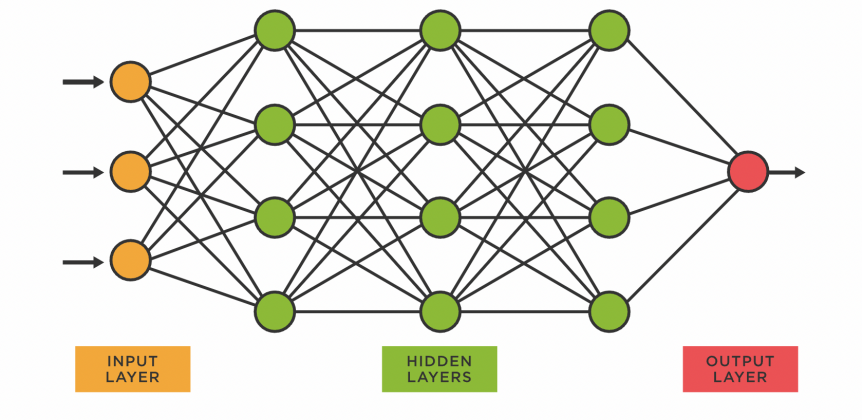
\includegraphics[width=0.9\linewidth]{gambar/bener/ArsitekturDeeplearning.png}
	\captionof{figure}{Deep Learning Layers}
	\label{fig:Deep Learning secara umum}
\end{figure}  
\textit{Deep learning} adalah salah satu cabang utama dalam bidang kecerdasan buatan yang bertujuan mengembangkan model komputasional berdasarkan arsitektur jaringan saraf tiruan atau yang biasa disebut sebagai \textit{neural networks} yang sangat dalam dan kompleks seperti pada Gambar \ref{fig:Deep Learning secara umum}. Tujuan utama dari \textit{deep learning} adalah menciptakan mesin-mesin yang dapat belajar secara mandiri melalui representasi data yang lebih abstrak dan terstruktur. Para peneliti dan ilmuwan dalam bidang ini berupaya meniru cara kerja otak manusia, khususnya dalam hal pemrosesan informasi dalam lapisan-lapisan yang semakin kompleks dan hierarkis. \textit{Deep Learning} bekerja dengan mengimplementasikan jaringan saraf tiruan yang terdiri dari banyak lapisan atau tingkatan, yang masing-masing lapisan berisi sejumlah neuron. Setiap neuron menerima input, mengalikan input dengan bobot yang ditentukan, menjumlahkan hasil perkalian, dan lalu melewatkan hasilnya melalui fungsi aktivasi yang menghasilkan output. Proses ini berulang melalui lapisan-lapisan hingga mencapai lapisan keluaran, di mana output akhir model diperoleh. \textit{Deep learning} berusaha meniru cara kerja otak manusia dengan memproses data secara hierarkis dan mempelajari representasi fitur dari data yang kompleks. \cite{patterson2017deep}

Pada awal pelatihan, bobot dan bias pada setiap neuron diinisialisasi secara acak. Kemudian, model diberi data latihan yang terdiri dari input dan output yang diharapkan. Selama pelatihan, model mengoptimalkan bobot dan biasnya dapat meminimalkan kesalahan antara output yang dihasilkan oleh model dan output yang diharapkan. Proses ini dilakukan menggunakan algoritma optimasi seperti \textit{Stochastic Gradient Descent (SGD)} atau varian lainnya. Proses pelatihan \textit{deep learning} melibatkan dua tahap utama: tahap maju \textit{(forward pass)} dan tahap mundur \textit{(backward pass)}. Pada tahap maju, input diteruskan melalui model dari lapisan masukan ke lapisan keluaran, menghasilkan prediksi model. Selama tahap mundur, kesalahan prediksi dibandingkan dengan output yang diharapkan, dan nilai gradien kesalahan dihitung mundur melalui jaringan. Gradien ini menunjukkan bagaimana bobot dan bias pada setiap neuron harus diubah agar kesalahan dapat diminimalkan. \cite{deng2014deep}

Dengan adanya gradien kesalahan, algoritma optimasi dapat diterapkan dalam memperbarui bobot dan bias pada setiap neuron. Proses ini disebut pembaruan parameter. Algoritma optimasi menggunakan gradien ini menyesuaikan bobot dan bias agar model semakin mendekati target yang diinginkan. Pelatihan \textit{deep learning} memerlukan banyak data dan komputasi yang kuat. Model \textit{deep learning} memiliki banyak parameter, dan agar mendapatkan hasil yang baik, perlu data pelatihan yang mencukupi agar model dapat menggeneralisasi dengan baik pada data baru. Selain itu, model \textit{deep learning} juga membutuhkan sumber daya komputasi yang besar, seperti GPU atau TPU, dalam rangka mengatasi kompleksitas perhitungan pada model yang dalam dan besar. Setelah model dilatih, ia dapat digunakan melakukan tugas-tugas tertentu seperti klasifikasi gambar, analisis teks, atau prediksi. Model \textit{deep learning} juga dapat disimpan dan digunakan kembali melakukan tugas-tugas serupa atau dimodifikasi dan disesuaikan dengan tugas yang berbeda. Sebagai subbidang dalam machine learning, \textit{deep learning} terus mengalami perkembangan pesat. Para peneliti terus mencari cara-cara agar meningkatkan efisiensi, akurasi, dan generalisasi model \textit{deep learning}. \cite{smith2007teaching}

Salah satu turunan dari \textit{deep learning} adalah \textit{convolutional neural networks (CNN)}. \textit{CNN} terbukti sangat efektif dalam menangani masalah pengenalan gambar karena menggunakan operasi konvolusi dalam mendeteksi fitur-fitur khusus di dalam gambar. Sebagai contoh, ketika melakukan klasifikasi gambar mobil, \textit{CNN} mampu belajar mengenali roda, pintu, dan bagian-bagian mobil lainnya yang relevan dalam mengidentifikasi jenis mobil tersebut. Turunan lainnya adalah \textit{recurrent neural networks (RNN)}, yang khusus digunakan sebagai data urutan atau sequential seperti teks dan suara. \textit{RNN} mempertahankan informasi sebelumnya dalam bentuk "memori" dan digunakan pada tugas-tugas seperti prediksi teks berikutnya dalam suatu kalimat atau bahkan menerjemahkan bahasa.

Salah satu contoh lain turunan dari \textit{deep learning} adalah \textit{Generative Adversarial Networks (GANs)}. \textit{GANs} adalah suatu jenis model \textit{deep learning} yang terdiri dari dua jaringan saraf tiruan yang saling bersaing: generator dan diskriminator. Generator bertugas membuat data baru yang menyerupai data pelatihan, sementara diskriminator bertugas membedakan data asli dari data yang dihasilkan oleh generator. Proses pelatihan \textit{GANs} berlangsung dalam dua tahap yang berulang: generator mencoba meningkatkan kualitas data yang dihasilkan agar dapat menipu diskriminator, sedangkan diskriminator terus belajar menjadi lebih baik dalam membedakan data asli dan palsu.

Contoh lainnya adalah \textit{Autoencoders}, yang merupakan jenis jaringan saraf tiruan yang diajarkan merekonstruksi data masukan sebagai outputnya sendiri. \textit{Autoencoders} terdiri dari dua bagian: encoder yang mengonversi data masukan menjadi representasi terkompresi dalam ruang fitur yang lebih rendah, dan decoder yang mengubah representasi terkompresi kembali ke dalam bentuk data semula. \textit{Autoencoders} sering digunakan dalam tugas-tugas seperti reduksi dimensi data (dimensionality reduction) dan denoising, di mana model ini belajar merepresentasikan data dalam bentuk yang lebih efisien dan tangguh terhadap noise. Turunan \textit{deep learning} lainnya adalah \textit{Long Short-Term Memory (LSTM)}, yang merupakan varian dari \textit{recurrent neural networks (RNN)} yang lebih mampu dalam mengatasi masalah vanishing gradient pada data urutan panjang. \textit{LSTM} memiliki mekanisme "gerbang" khusus yang memungkinkannya menyimpan informasi dalam waktu yang lebih lama dan mengatur aliran informasi pada lapisan tersembunyi. Akibatnya, \textit{LSTM} menjadi populer dalam aplikasi NLP seperti penerjemahan mesin, pembangkitan teks, dan analisis sentimen.

\textit{Deep learning} telah berhasil diimplementasikan dalam berbagai bidang dan memberikan dampak yang signifikan. Salah satu contoh implementasi \textit{deep learning} yang menonjol adalah di bidang pengenalan gambar dan pengolahan citra. Model \textit{deep learning} seperti \textit{Convolutional Neural Networks (CNN)} telah digunakan melakukan klasifikasi gambar, deteksi objek, dan segmentasi citra. Misalnya, aplikasi pengenalan wajah di perangkat lunak atau perangkat keamanan yang dapat mengidentifikasi individu berdasarkan fitur wajahnya. Dalam bidang kesehatan, \textit{deep learning} telah digunakan mendukung diagnosis medis dan penelitian. Model \textit{deep learning} telah diterapkan dalam mendeteksi penyakit dari gambar medis seperti \textit{X-ray},\textit{ CT scan}, atau MRI. Selain itu, \textit{deep learning} juga digunakan dalam analisis citra histopatologi membantu mendiagnosis kanker dan penyakit lainnya. Penerapan \textit{deep learning} juga dapat ditemukan di bidang otomotif, khususnya dalam pengembangan kendaraan otonom. Model \textit{deep learning} seperti \textit{CNN} dan \textit{LSTM} digunakan mengenali objek di sekitar kendaraan, memprediksi perilaku pengendara, dan membantu dalam mengambil keputusan saat berkendara.

Dalam industri keuangan, \textit{deep learning} telah digunakan dalam analisis data keuangan dan prediksi pasar. Model \textit{deep learning} dapat mengidentifikasi pola kompleks dari data pasar dan membantu investor atau trader dalam membuat keputusan investasi. Penerapan \textit{deep learning} juga ditemukan dalam aplikasi \textit{NLP (Natural Language Processing)}. Model \textit{deep learning} seperti \textit{Transformer} telah digunakan dalam penerjemahan bahasa, generasi teks, analisis sentimen, dan \textit{chatbot}. Selain itu, \textit{deep learning} juga telah diadopsi dalam berbagai aplikasi industri seperti manufaktur, pertanian, energi, dan lainnya. Misalnya, dalam industri manufaktur, \textit{deep learning} digunakan dalam mengoptimalkan proses produksi dan memprediksi kerusakan pada mesin. Di bidang pertanian, \textit{deep learning} digunakan mendeteksi hama dan penyakit tanaman, serta memantau pertumbuhan tanaman secara akurat. Implementasi \textit{deep learning} terus berkembang seiring dengan kemajuan teknologi dan kebutuhan mengatasi tantangan dalam berbagai industri. Penggunaan \textit{deep learning} yang semakin luas memberikan potensi mengubah cara kerja dan memberikan solusi yang lebih efektif dalam berbagai aspek kehidupan manusia.

\subsection{Convolutional Neural Network (CNN)}
\begin{figure}[hbt!]
  \centering
  % Nama dari file gambar yang diinputkan
  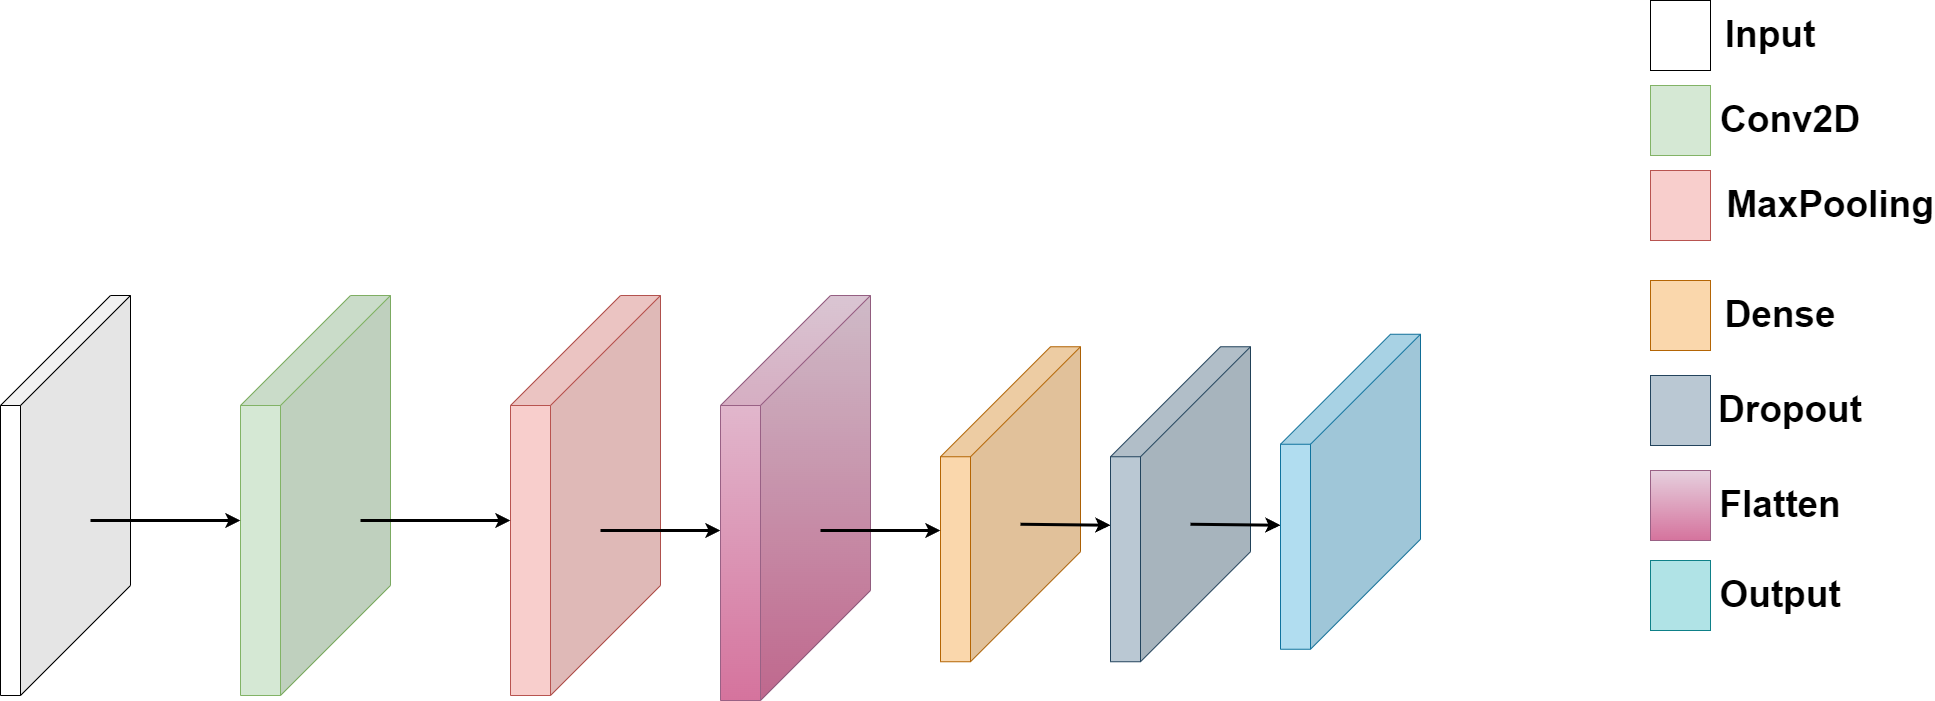
\includegraphics[width=0.8\linewidth]{gambar/bener/Arsitektur_CNN_Umum.png}
  % Keterangan gambar yang diinputkan
  \captionof{figure}{Arsitektur CNN}
  % Label referensi dari gambar yang diinputkan
  \label{fig:Arsitektur Umum Convolutional Neural Network}
\end{figure}
\textit{Convolutional Neural Network (CNN)} adalah sebuah jenis arsitektur model \textit{deep learning} yang khusus dirancang melaksanakan tugas-tugas pengolahan citra dan analisis visual. Inspirasi utama dari \textit{CNN} berasal dari cara otak manusia, khususnya korteks visual, memproses dan memahami informasi visual. Dengan menggunakan lapisan-lapisan konvolusi, \textit{CNN} dapat secara efektif dan efisien mengidentifikasi fitur-fitur penting dalam gambar secara hierarkis. Fungsi utama lapisan konvolusi dalam \textit{CNN} seperti pada \ref{fig:Arsitektur Umum Convolutional Neural Network}
adalah mendeteksi pola-pola spesifik atau fitur-fitur visual pada data input. Lapisan konvolusi dilengkapi dengan filter atau kernel kecil yang bergeser secara bertahap di seluruh citra agar menghasilkan peta fitur yang mencerminkan kehadiran fitur-fitur tersebut. Misalnya, filter pertama mungkin berfokus pada deteksi tepi dan garis, sementara filter berikutnya dapat mengenali sudut atau bentuk yang lebih kompleks. \cite{wu2017introduction}

Setelah melalui lapisan konvolusi, data diproses melalui lapisan aktivasi seperti \textit{ReLU (Rectified Linear Unit)}. Fungsi aktivasi ini membantu memperkenalkan non-linearitas ke dalam model, memungkinkan \textit{CNN} mempelajari representasi fitur yang lebih kompleks dan abstrak. Proses konvolusi dan aktivasi berulang pada lapisan-lapisan berikutnya, dengan setiap lapisan mencoba memahami dan mengekstraksi fitur-fitur semakin tingkat tinggi dari peta fitur sebelumnya. Selain lapisan konvolusi, \textit{CNN} juga mengandung lapisan-lapisan lain seperti \textit{pooling layer} dan \textit{fully connected layer}. \textit{Pooling layer} bertujuan mereduksi dimensi spasial dari peta fitur, mengurangi jumlah parameter dan mencegah overfitting. Kemudian, data hasil pooling diubah menjadi vektor dan diproses melalui \textit{fully connected layer} melakukan tugas klasifikasi atau regresi. \cite{koushik2016understanding}

Kekuatan utama dari \textit{CNN} adalah kemampuannya secara otomatis dan adaptif mempelajari representasi fitur dari data input. Dengan mendeteksi dan memahami fitur-fitur kunci dari gambar secara hierarkis, \textit{CNN} dapat menghasilkan prediksi atau output yang akurat dalam berbagai tugas analisis visual. Penggunaan teknologi \textit{deep learning} seperti \textit{CNN} telah menghadirkan perubahan signifikan dalam berbagai industri dan bidang, menciptakan solusi baru dan aplikasi yang inovatif dalam mengatasi masalah-masalah kompleks. Terus berlanjutnya penelitian dan pengembangan di bidang \textit{deep learning} diharapkan akan membuka lebih banyak potensi implementasi dan penerapan \textit{CNN} dalam berbagai konteks dan permasalahan dunia nyata. Contoh implementasi \textit{CNN} sangat beragam dan telah berhasil diterapkan dalam berbagai bidang. Misalnya, dalam klasifikasi gambar, \textit{CNN} telah digunakan ketika mengenali objek-objek pada gambar seperti manusia, mobil, atau binatang. Di bidang medis, \textit{CNN} dapat membantu dalam deteksi dan diagnosis penyakit berdasarkan gambar medis seperti X-ray atau MRI. Selain itu, dalam industri otomotif, \textit{CNN} digunakan dalam pengembangan kendaraan otonom agar bisa mendeteksi dan mengenali objek di sekitar kendaraan.

Implementasi dari \textit{Convolutional Neural Network (CNN)} telah menjadi salah satu pendorong utama dalam perkembangan teknologi dan aplikasi visual yang revolusioner. Dalam bidang komputer visi, \textit{CNN} telah digunakan dalam berbagai aplikasi seperti deteksi objek, segmentasi citra, dan rekonstruksi gambar. Penggunaan \textit{CNN} dalam industri otomotif juga semakin populer dalam pengembangan kendaraan otonom, di mana \textit{CNN} digunakan saat mendeteksi dan mengenali objek di sekitar kendaraan seperti pejalan kaki, kendaraan lain, dan rambu lalu lintas. Di bidang kesehatan, \textit{CNN} telah menemukan penerapan yang luas dalam analisis citra medis, termasuk deteksi kanker, segmentasi organ, dan pengenalan pola patologis. \textit{CNN} telah membantu mempercepat dan meningkatkan akurasi diagnosa medis, membuka peluang dalam penanganan penyakit secara lebih dini dan tepat.

Selain itu, aplikasi \textit{CNN} juga dapat ditemukan dalam industri hiburan dan kreatif. \textit{CNN} digunakan dalam teknologi realitas virtual dan \textit{augmented reality} ketika melacak gerakan pengguna dan mengintegrasikan objek virtual ke dalam lingkungan nyata. Dalam industri film dan animasi, \textit{CNN} memungkinkan penciptaan efek visual yang menakjubkan dan realistis. Penggunaan teknologi \textit{deep learning}, termasuk \textit{CNN}, telah memberikan dampak signifikan dalam bidang kecerdasan buatan dan telah menciptakan kemajuan besar dalam berbagai industri. Contoh arsitektur dari \textit{CNN} yang terkenal adalah \textit{LeNet-5}, yang dikembangkan oleh Yann LeCun pada tahun 1998 mengenali karakter tulisan tangan. Arsitektur \textit{LeNet-5} terdiri dari dua lapisan konvolusi yang diikuti oleh lapisan pooling dan lapisan terhubung penuh. \textit{LeNet-5} berhasil memperkenalkan konsep konvolusi dalam dunia pengolahan citra dan memberikan dasar bagi pengembangan model \textit{CNN} lebih lanjut.

Selanjutnya, ada arsitektur \textit{AlexNet} yang dikembangkan oleh Alex Krizhevsky, Ilya Sutskever, dan Geoffrey Hinton pada tahun 2012. \textit{AlexNet} merupakan salah satu arsitektur yang mempopulerkan penggunaan \textit{deep learning}, terutama \textit{CNN}, dalam tugas klasifikasi gambar. \textit{AlexNet} berhasil meraih kemenangan besar dalam kompetisi \textit{ImageNet} dengan performa yang jauh lebih baik dari metode konvensional pada saat itu. Selanjutnya, arsitektur \textit{VGGNet} dikembangkan oleh Karen Simonyan dan Andrew Zisserman pada tahun 2014. \textit{VGGNet} terkenal dengan kedalaman yang lebih besar, terdiri dari 16 atau 19 lapisan konvolusi, yang membantu meningkatkan akurasi dalam klasifikasi gambar dengan biaya komputasi yang lebih tinggi.

Contoh lainnya adalah arsitektur \textit{GoogLeNet} yaitu \textit{Inception} yang dikembangkan oleh tim dari \textit{Google} pada tahun 2014. \textit{GoogLeNet} memperkenalkan modul \textit{Inception} yang mencakup beberapa operasi konvolusi dalam paralel, mengoptimalkan kompromi antara akurasi dan efisiensi komputasi.Sejak saat itu, muncul berbagai arsitektur CNN lainnya, seperti \textit{ResNet}, \textit{DenseNet}, dan \textit{MobileNet}, yang terus mengalami pengembangan memenuhi kebutuhan beragam dalam berbagai aplikasi dan mendapatkan hasil yang lebih baik dalam analisis visual.

\subsubsection{ResNet50v2}
\textit{ResNet50V2} adalah salah satu model arsitektur \textit{Convolutional Neural Network (CNN)} yang merupakan variasi dari ResNet50, yang dikembangkan oleh Kaiming He dan timnya pada tahun 2015. ResNet sendiri merupakan singkatan dari \textit{Residual Network} yang merupakan terobosan dalam pengembangan jaringan saraf yang sangat dalam. Masalah utama yang diatasi oleh ResNet adalah pemudaran gradien yang sering terjadi pada jaringan yang dalam, yang menyebabkan kesulitan dalam pelatihan dan pengoptimalan model. \textit{ResNet50V2} menggunakan teknik \textit{Skip Connection} atau \textit{Residual Connections} mengatasi masalah pemudaran gradien ini. \cite{rahimzadeh2020modified} . Cara kerja \textit{ResNet50V2} seperti pada Gambar \ref{fig:ArsitekturResNet50V2}
dimulai dengan lapisan konvolusi pertama melakukan ekstraksi fitur dari gambar input. Setelah itu, model menggunakan beberapa blok residual bertingkat agar mempelajari representasi fitur yang semakin kompleks. Blok residual adalah inti dari arsitektur ResNet, yang memungkinkan aliran informasi yang lancar melalui lapisan-lapisan jaringan. \textit{Skip connections} memungkinkan input lompat langsung ke lapisan yang lebih dalam, atau ditambahkan ke output lapisan tersebut, sehingga memungkinkan model mempertahankan informasi asli selama proses pembelajaran.

\begin{figure}[!hbt]
  \centering
  % Nama dari file gambar yang diinputkan
  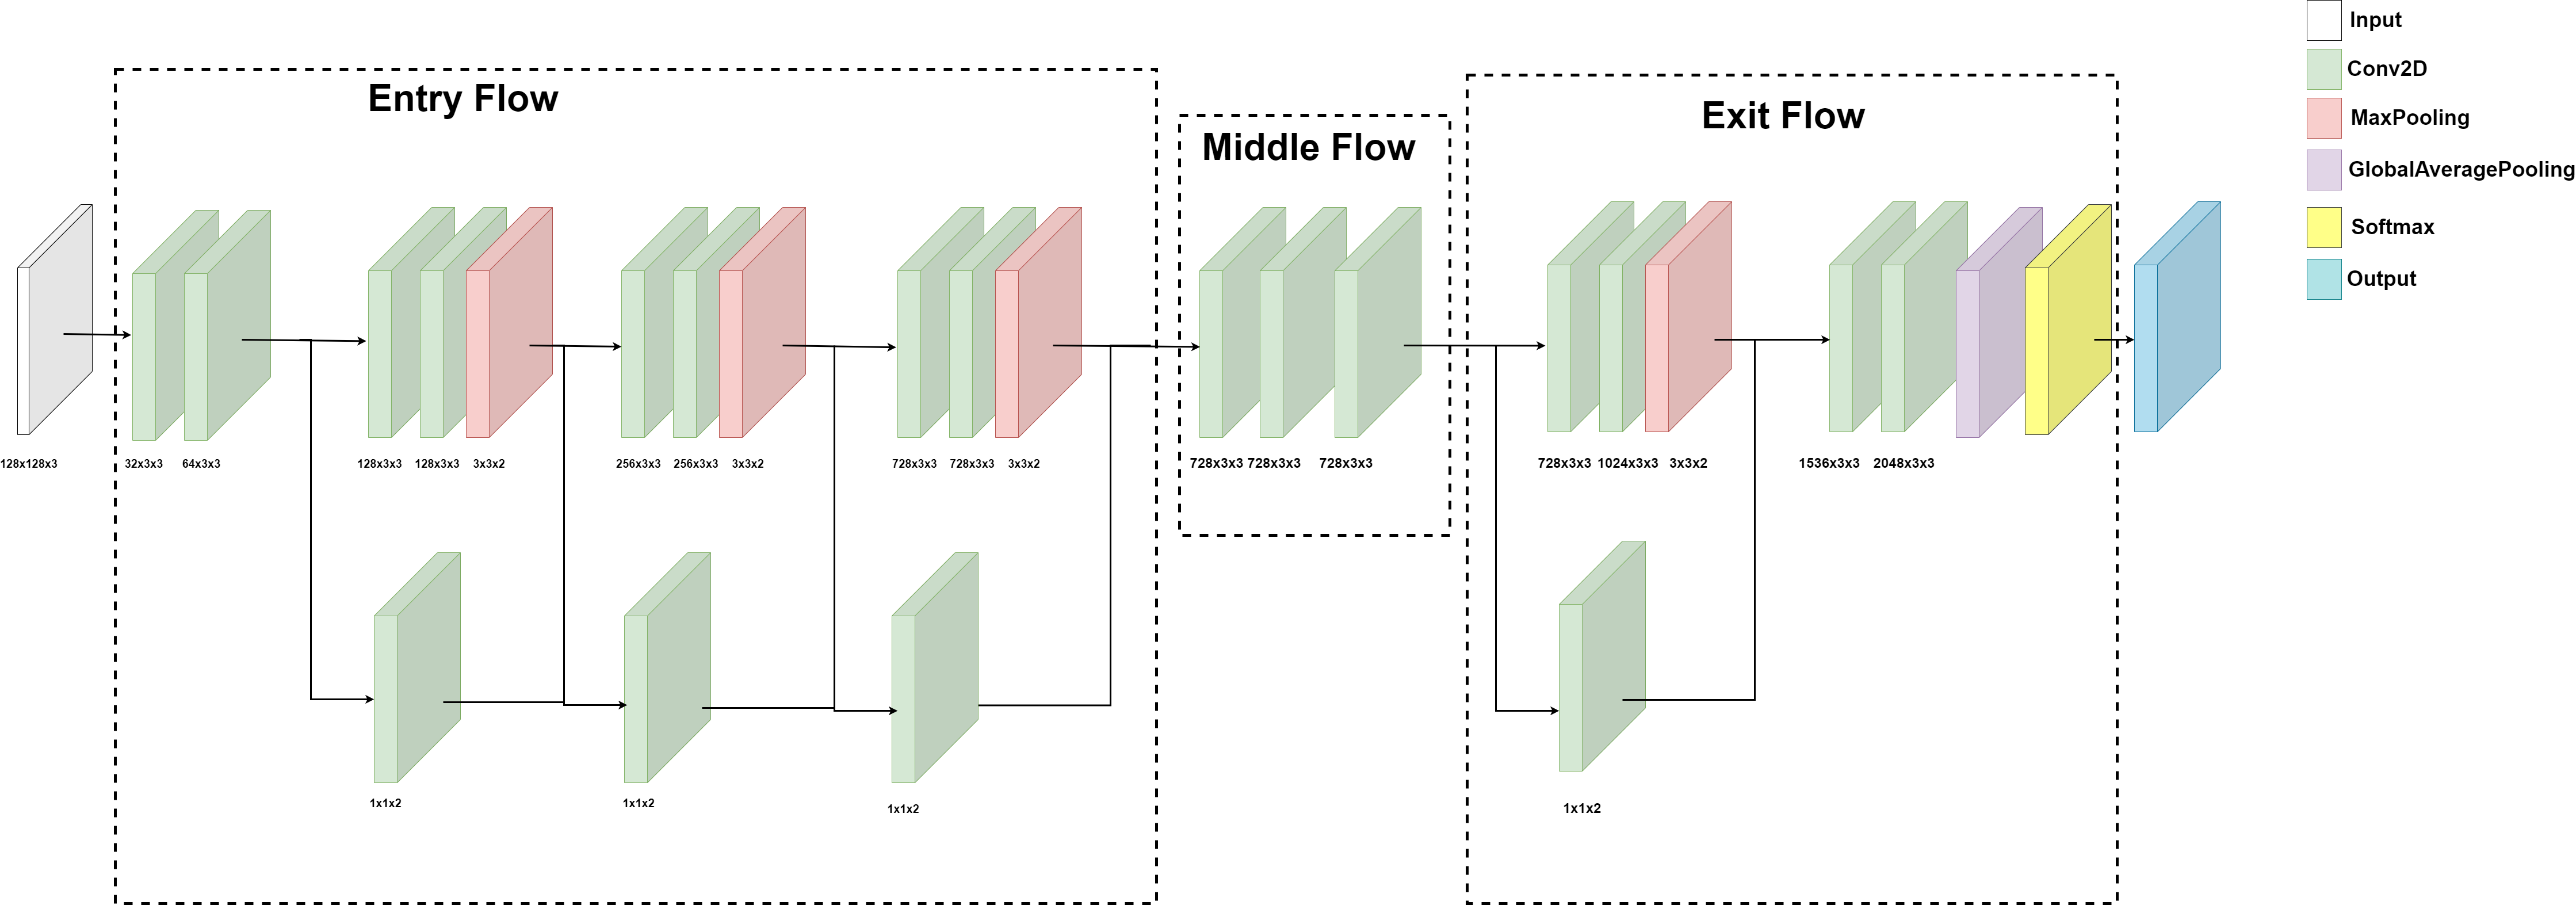
\includegraphics[width=0.8\linewidth]{gambar/bener/Arsitektur_ModelCNNResNet50V2_Dasar.png}
  % Keterangan gambar yang diinputkan
  \captionof{figure}{Arsitektur CNN ResNet50V2}
  % Label referensi dari gambar yang diinputkan
  \label{fig:ArsitekturResNet50V2}
\end{figure}

Dengan menggunakan blok residual dan \textit{skip connections}, \textit{ResNet50V2} dapat mengatasi masalah pemudaran gradien dengan lebih efektif. Gradien adalah indikator bagaimana model merespons perubahan parameter selama proses pelatihan. Pemudaran gradien terjadi ketika nilai gradien menjadi sangat kecil atau bahkan menghilang saat melewati lapisan-lapisan dalam jaringan. Dalam jaringan yang sangat dalam, pemudaran gradien dapat menyebabkan kesulitan dalam mengoptimalkan parameter dan memperlambat proses pelatihan. Namun, dengan adanya \textit{skip connections}, informasi dapat lebih mudah mengalir mundur melalui jaringan, mengurangi pemudaran gradien dan mempercepat pelatihan. \cite{prusty2022resnet50v2} . Selain itu, \textit{ResNet50V2} menggunakan blok \textit{"bottle-neck"} yang terdiri dari tiga lapisan konvolusi dengan ukuran kernel yang berbeda, yaitu 1x1, 3x3, dan 1x1. Penggunaan blok \textit{bottle-neck} ini mengurangi dimensi fitur di tengah blok, mengurangi kompleksitas komputasi dan jumlah parameter yang diperlukan. Dengan demikian, \textit{ResNet50V2} memiliki struktur yang lebih efisien dan dapat menghasilkan representasi fitur yang lebih kuat dengan meminimalkan biaya komputasi.

Selain teknik \textit{skip connections} dan blok \textit{bottle-neck}, \textit{ResNet50V2} juga menerapkan normalisasi batch (batch normalization) dan fungsi aktivasi \textit{ReLU} (Rectified Linear Unit) pada setiap lapisan konvolusi. Normalisasi batch membantu meningkatkan kestabilan dan kemampuan pembelajaran jaringan, sementara \textit{ReLU} berfungsi memperkenalkan non-linearitas dan meningkatkan representasi fitur yang dapat dipelajari oleh model. \textit{ResNet50V2} telah terbukti menjadi salah satu arsitektur yang sangat efektif dalam berbagai tugas pengolahan citra dan visi komputer. Model ini telah digunakan dalam banyak kompetisi dan tugas benchmark, menghasilkan performa yang luar biasa dalam klasifikasi gambar, deteksi objek, dan tugas-tugas visual lainnya. Dengan menggunakan kombinasi teknik canggih seperti skip connections, blok \textit{bottle-neck}, normalisasi batch, dan fungsi aktivasi \textit{ReLU}, \textit{ResNet50V2} berhasil mencapai tingkat akurasi yang tinggi dalam berbagai skenario dan aplikasi, menjadi salah satu pilihan utama terkait masalah pengolahan citra yang kompleks.

\subsubsection{Xception}
Arsitektur \textit{Xception} adalah inovasi dalam desain jaringan saraf tiruan yang menawarkan solusi efisiensi komputasi dan kinerja yang tinggi dalam tugas pengolahan citra. Cara kerja arsitektur \textit{Xception} berfokus pada penggunaan konsep konvolusi yang dapat dipisahkan secara mendalam agar mengurangi beban komputasi dan jumlah parameter dalam model. Ini menghasilkan model yang lebih ringkas dan cepat, sehingga lebih mudah dijalankan pada perangkat dengan sumber daya terbatas.

Konsep utama di balik \textit{Xception} adalah menggantikan operasi konvolusi standar dalam modul \textit{Inception} dengan konvolusi yang dapat dipisahkan secara mendalam seperti pada Gambar \ref{fig:ArsitekturXception}
. Modul \textit{Inception} adalah bagian kunci dari arsitektur jaringan \textit{Inception}, yang menggunakan berbagai ukuran \textit{filter} dalam paralel dalam mengekstraksi fitur dari gambar input. Dengan menggunakan konvolusi yang dapat dipisahkan secara mendalam, \textit{Xception} memisahkan operasi konvolusi menjadi dua tahap: konvolusi \textit{depthwise} dan konvolusi \textit{pointwise}.Pada tahap konvolusi \textit{depthwise}, satu \textit{filter} digunakan setiap lapisan input. Konvolusi ini dilakukan secara terpisah bagi setiap kanal warna (depth) gambar, yang menghasilkan output berukuran tinggi x lebar x kedalaman. Output dari langkah ini akan menjadi input dari tahap konvolusi \textit{pointwise}. Pada tahap konvolusi \textit{pointwise}, \textit{filter} dengan ukuran 1x1xkedalaman digunakan menghasilkan beberapa fitur. Penggunaan konvolusi 1x1 ini memungkinkan model melakukan operasi linier pada data input menghasilkan representasi fitur yang lebih kompleks.

\begin{figure}[!hbt]
  \centering
  % Nama dari file gambar yang diinputkan
  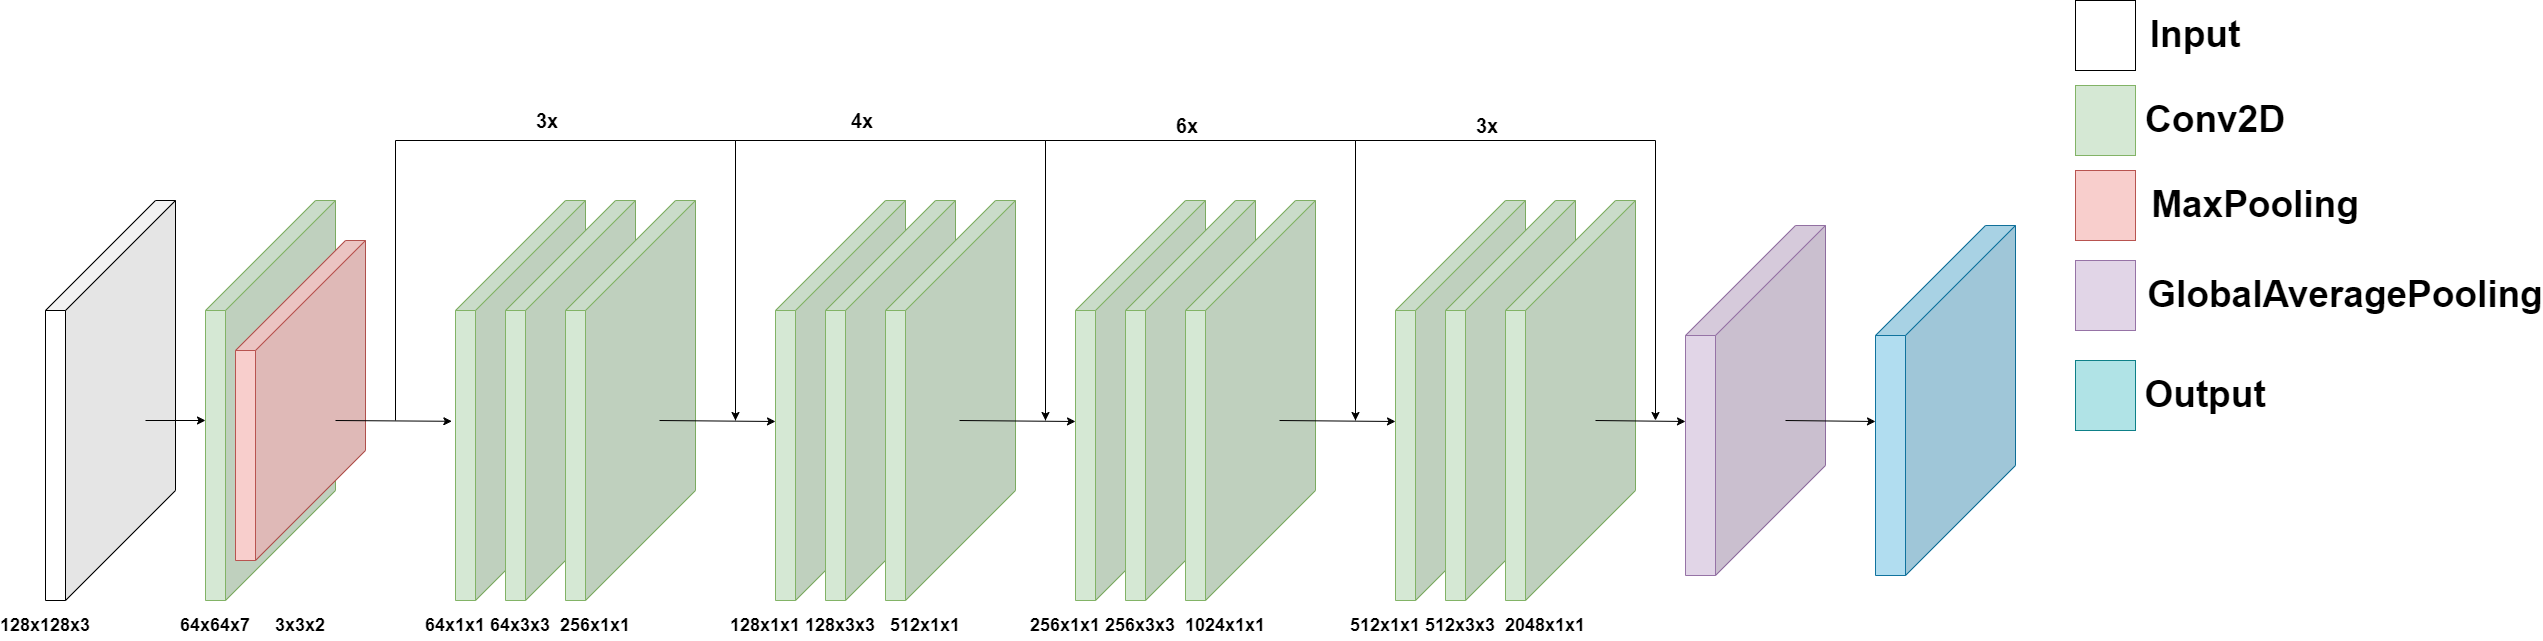
\includegraphics[width=0.8\linewidth]{gambar/bener/Arsitektur_CNNXception.png}
  % Keterangan gambar yang diinputkan
  \captionof{figure}{Arsitektur CNN Xception}
  % Label referensi dari gambar yang diinputkan
  \label{fig:ArsitekturXception}
\end{figure}
Struktur arsitektur \textit{Xception} terdiri dari tiga modul utama: \textit{entry flow}, \textit{middle flow}, dan \textit{exit flow}. \textit{Entry flow} terdiri dari konvolusi normal diikuti oleh konvolusi yang dapat dipisahkan secara mendalam. Modul ini bertanggung jawab menginisialisasi fitur-fitur penting dari gambar input. Selanjutnya, \textit{middle flow} terdiri dari 8 miniblock, setiap miniblock terdiri dari 3 konvolusi yang dapat dipisahkan secara mendalam. Modul ini bertanggung jawab melakukan proses ekstraksi fitur yang lebih mendalam dan kompleks dari gambar. Terakhir, \textit{exit flow} terdiri dari konvolusi yang dapat dipisahkan secara mendalam, feature flattening, dan output. Modul ini bertanggung jawab menghasilkan hasil akhir dari model, seperti prediksi kelas dalam tugas klasifikasi gambar.

Dengan menggunakan teknik konvolusi yang dapat dipisahkan secara mendalam, \textit{Xception} berhasil mengurangi jumlah parameter yang diperlukan dalam model dan meningkatkan efisiensi komputasi. Dalam model yang lebih dalam dan kompleks, jumlah perkalian matriks yang diperlukan melakukan konvolusi dapat sangat besar, menyebabkan model menjadi lebih lambat dan membutuhkan lebih banyak sumber daya komputasi. Dengan menggunakan konsep konvolusi yang dapat dipisahkan secara mendalam, \textit{Xception} mengurangi beban komputasi ini, sehingga model dapat dijalankan dengan lebih cepat dan lebih efisien.

Dalam berbagai tugas pengolahan citra, \textit{Xception} telah terbukti memberikan hasil yang sangat baik dan akurasi yang tinggi. Model ini telah digunakan dalam berbagai kompetisi dan benchmark, menunjukkan kinerja yang unggul dalam klasifikasi gambar, deteksi objek, segmentasi citra, dan tugas visual lainnya. Kemampuan \textit{Xception} menghasilkan representasi fitur yang kuat dan kompresi model yang efisien menjadikannya pilihan utama dalam berbagai aplikasi pengolahan citra dan visi komputer. Dengan terus berkembangnya teknologi deep learning, \textit{Xception} terus menjadi subjek penelitian dan pengembangan meningkatkan performa dan kemampuannya dalam berbagai tugas pengolahan citra yang semakin kompleks dan realistis.





  % Konten metodologi
  \section{METODOLOGI}

% Ubah konten-konten berikut sesuai dengan isi dari metodologi

\subsection{Metode yang digunakan}

Penelitian ini mengikuti metode untuk pengerjaan nya menguki sesuai yang sudah dirancang sebagai berikut

% Contoh input gambar dengan format *.jpg
\begin{figure} [ht] \centering
  % Nama dari file gambar yang diinputkan
  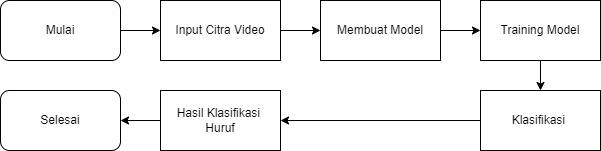
\includegraphics[scale=0.45]{gambar/Metodologi_TA.jpg}
  % Keterangan gambar yang diinputkan
  \caption{\emph{Blueprint} Metodologi Pengerjaan}
  % Label referensi dari gambar yang diinputkan
  \label{fig:Blueprint}
\end{figure}

\subsubsection{Input Citra Video}
Pada tahapan ini , Kamera Webcam akan melakukan deteksi terhadap gestur yang diperagakan . Disini digunakan Library OpenCV dalam rangka untuk membantu menangkap frame yang terdapat di Video 

\subsubsection{Membuat Model}
\begin{figure} [ht] \centering
  % Nama dari file gambar yang diinputkan
  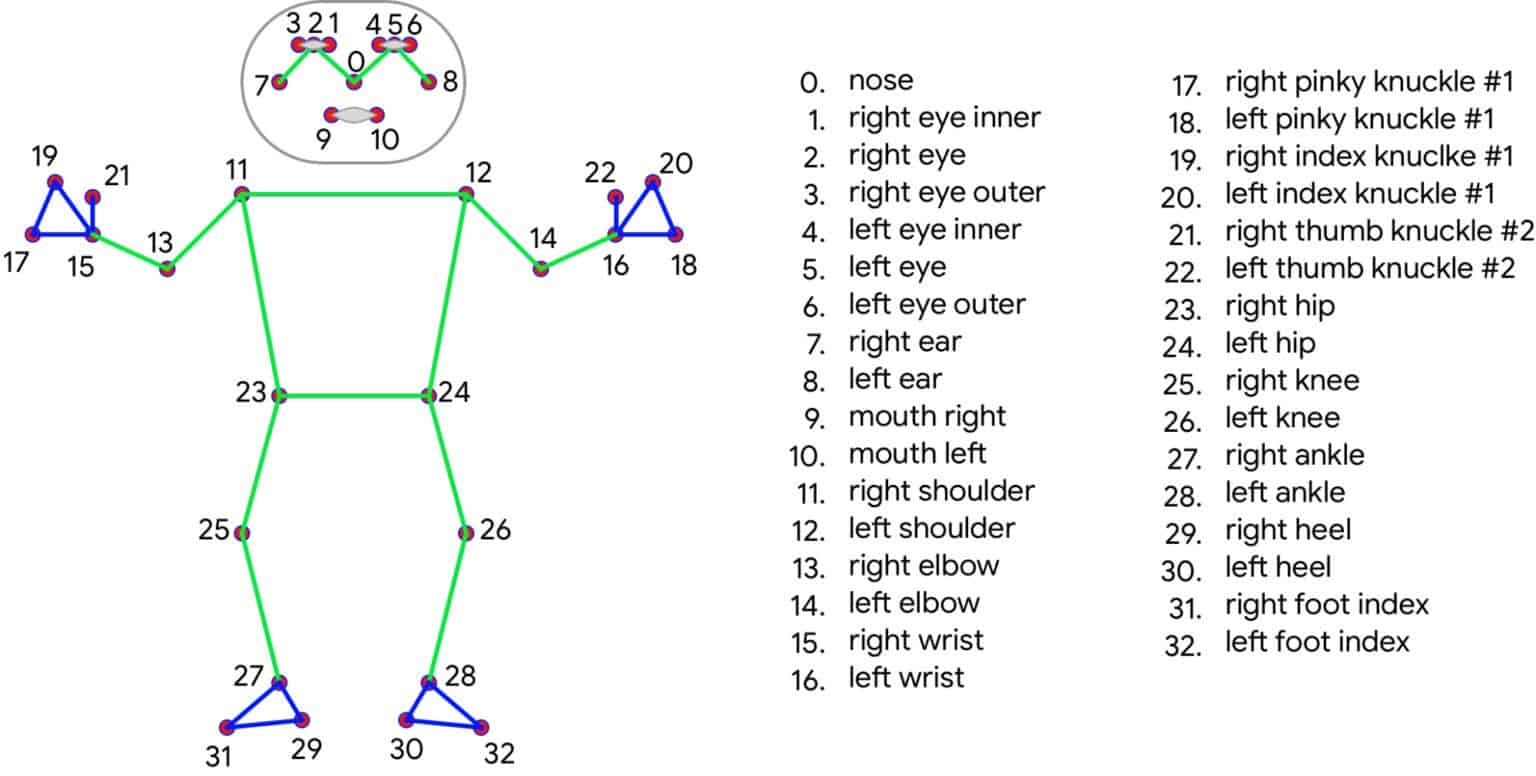
\includegraphics[scale=0.15]{gambar/humanpose.jpg}
  % Keterangan gambar yang diinputkan
  \caption{Model Human Pose dari MediaPipe}
  % Label referensi dari gambar yang diinputkan
  \label{fig:Blueprint}
\end{figure}
Berikutnya dilakukan pembuatan model HumanPose dengan memanfaatkan MediaPipe . Hal ini bertujuan untuk membantu melakukan identifikasi bagian-bagian tubuh manusia dalam citra atau video dalam rangka memperkuat akurasi 

\subsubsection{Training Model}
Selanjutnya dilakukan proses pembelajaran yang digunakan untuk  kemampuan jaringan untuk mengenali dan memprediksi pola dan fitur yang relevan dari input yang diberikan. Training Model menggun

\subsubsection{Klasifikasi}
Setelah dilakukan nya training model sebelumnya menggunakan metode Convolutional Neural Network yang dibantu dengan Estimasi Pose yang dibantu oleh MediaPipe . Klasifikasi ini bertujuan untuk membagi suatu objek ke dalam kelas-kelas tertentu berdasarkan fitur yang dimilikinya

\subsubsection{Hasil Klasifikasi Huruf}
Setelah dilakukan klasifikasi pose semaphore maka didapatkan hasil huruf untuk dikenali
% Contoh penggunaan referensi dari gambar yang diinputkan
% Pada \emph{blueprint} yang tertera di Gambar \ref{fig:Blueprint}. \lipsum[12]

\subsection{Bahan dan peralatan yang digunakan}

\lipsum[13]

\subsection{Urutan pelaksanaan penelitian}

% Ubah tabel berikut sesuai dengan isi dari rencana kerja
\newcommand{\w}{}
\newcommand{\G}{\cellcolor{gray}}
\begin{table}[h!]
  \begin{tabular}{|p{3.5cm}|c|c|c|c|c|c|c|c|c|c|c|c|c|c|c|c|}

    \hline
    \multirow{2}{*}{Kegiatan} & \multicolumn{16}{|c|}{Minggu} \\
    \cline{2-17} &
    1 & 2 & 3 & 4 & 5 & 6 & 7 & 8 & 9 & 10 & 11 & 12 & 13 & 14 & 15 & 16 \\
    \hline

    % Gunakan \G untuk mengisi sel dan \w untuk mengosongkan sel
    Pengambilan data &
    \G & \G & \G & \G & \w & \w & \w & \w & \w & \w & \w & \w & \w & \w & \w & \w \\
    \hline

    Pengolahan data &
    \w & \w & \w & \w & \G & \G & \G & \G & \w & \w & \w & \w & \w & \w & \w & \w \\
    \hline

    Analisa data &
    \w & \w & \w & \w & \w & \w & \w & \w & \G & \G & \G & \G & \w & \w & \w & \w \\
    \hline

    Evaluasi penelitian &
    \w & \w & \w & \w & \w & \w & \w & \w & \w & \w & \w & \w & \G & \G & \G & \G \\
    \hline

  \end{tabular}
\end{table}

  % Konten lainnya
  \chapter{HASIL DAN PEMBAHASAN}
Pada bab ini dibahas mengenai pengujian dari aplikasi yang telah dikembangkan untuk mengetahui performa aplikasi dalam mendeteksi pose semaphore sesuai tujuan dari penelitian ini, sebagai upaya menciptakan aplikasi yang dapat melakukan prediksi pose semaphore berbasis Deep Learning.

\section{Dataset}
Dalam penelitian ini, dilakukan pengujian terhadap dataset citra yang terdiri dari 26 huruf alfabet yang umum digunakan sehari-hari. Dataset tersebut digunakan untuk melatih dan menguji model dalam mengenali huruf-huruf tersebut. Setiap huruf alfabet direpresentasikan oleh 1000 citra dalam dataset yang digunakan. Pengujian dilakukan untuk mengukur performa dan keakuratan model dalam mengenali huruf-huruf tersebut.

\begin{figure}[!hbt]
	\centering
	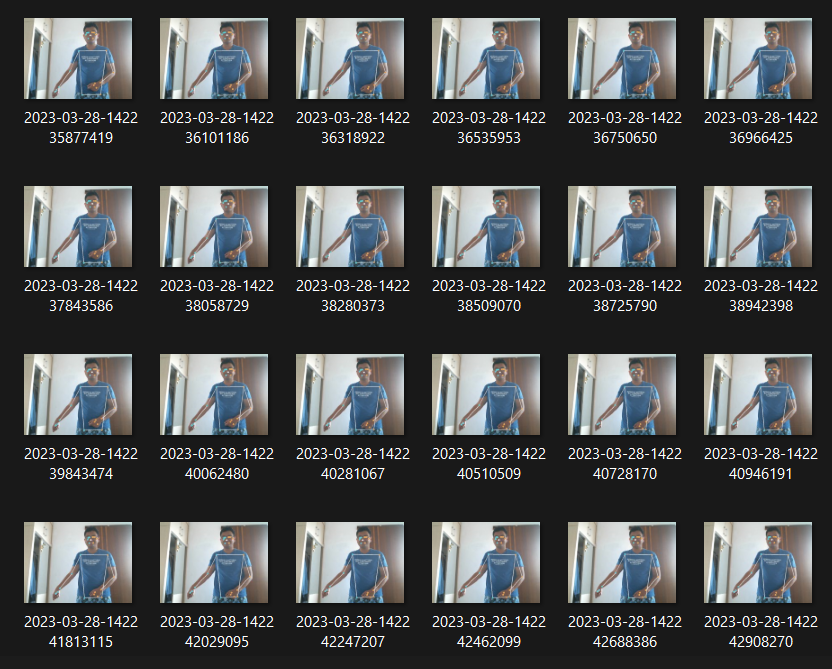
\includegraphics[width=0.7\linewidth]{gambar/citra_dataset.png}
	\captionof{figure}{Dataset Sebelum Ekstraksi}
	\label{fig:Datasetraw}
\end{figure}

Dataset awal yang terdiri dari gambar dan skeleton yang dikombinasikan, yang awalnya diperoleh melalui MediaPipe, akan melalui proses ekstraksi. Proses ekstraksi dilakukan menggunakan program yang telah dikembangkan, menghasilkan skeleton dengan latar belakang hitam. Hasil ekstraksi ini dapat dilihat dalam Gambar \ref{fig:Datasetekstark}.

\begin{figure}[!hbt]
	\centering
	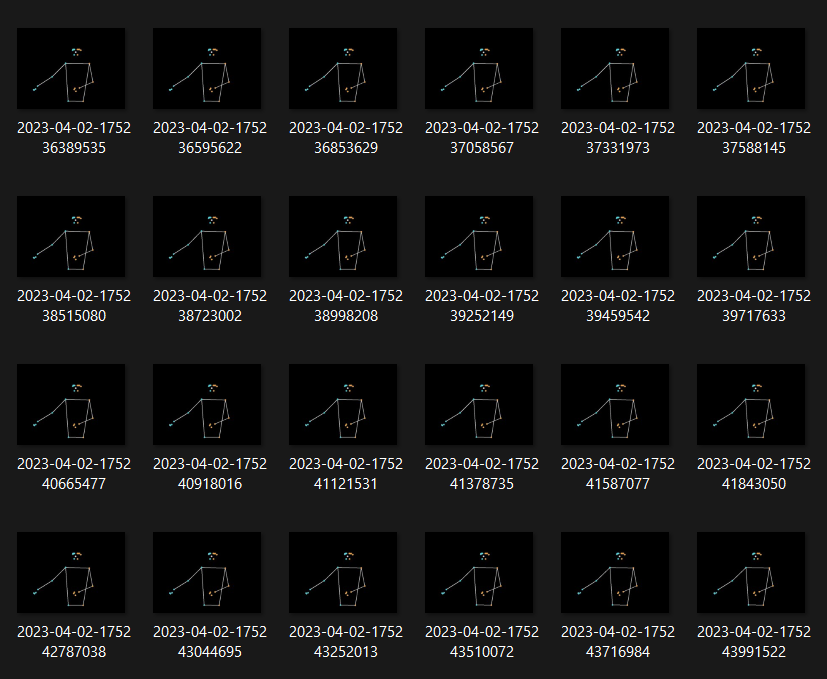
\includegraphics[width=0.7\linewidth]{gambar/tugas-akhir-dawe.png}
	\captionof{figure}{Ekstraksi dari Dataset awal}
	\label{fig:Datasetekstark}
\end{figure}
Dataset yang telah diekstrak ini dijadikan sebagai input dari model-model deep learning pada penelitian ini untuk training dan validasi. 

\begin{table}[htbp]
	\centering
	\captionof{table}{Daftar Dataset}
	\label{tab:datasethuruf}
	\begin{tabular}{|c|c|c|c|c|}
		\hline
		A & B & C & D & E \\
		\hline
		F & G & H & I & J \\
		\hline
		K & L & M & N & O \\
		\hline
		P & Q & R & S & T \\
		\hline
		U & V & W & X & Y \\
		\hline
		Z &   Akhir &   &   &   \\
		\hline
	\end{tabular}
\end{table}

Adapun huruf yang digunakan sebagai dataset bisa dilihat pada tabel \ref{tab:datasethuruf} . Dimana seluruh huruf memiliki bentuk yang statik atau tidak berubah

\section{Model CNN}

Pada awalnya, fungsi ini menerima parameter JumlahKelas yang mengindikasikan jumlah kelas dalam dataset yang digunakan. Kemudian, dilakukan inisialisasi input layer dengan ukuran (128, 128, 3) yang sesuai dengan dimensi gambar pada dataset.

Selanjutnya, dilakukan serangkaian operasi \textit{Conv2D}  dan \textit{MaxPooling2D}. Pertama, terdapat tiga layer \textit{Conv2D} yang masing-masing memiliki 32 \textit{neuron} dengan \textit{filter} berukuran 3x3. Aktivasi \textit{ReLU}  digunakan untuk mengaktifkan \textit{neuron}-\textit{neuron} tersebut. \textit{Padding} 'same' juga diterapkan agar ukuran output tetap sama dengan input. Setelah setiap layer \textit{Conv2D}, dilakukan \textit{MaxPooling2D} dengan ukuran \textit{pooling} 2x2 dan \textit{padding} 'same' untuk melakukan \textit{downsampling} dan mengurangi dimensi data.

Selanjutnya, dilakukan layer \textit{Conv2D} lagi dengan 16 \textit{neuron} dan \textit{filter} berukuran 3x3, diikuti oleh \textit{MaxPooling2D} dengan ukuran \textit{pooling} 2x2 dan \textit{padding} 'same'. Langkah ini bertujuan untuk mengekstraksi fitur-fitur yang lebih kompleks dari data.

Setelah melalui serangkaian operasi \textit{Conv2D} dan \textit{MaxPooling2D}, data kemudian diflatten menjadi vektor satu dimensi menggunakan layer Flatten. Hal ini diperlukan agar data dapat dimasukkan ke dalam layer \textit{Dense} yang merupakan layer \textit{fully connected}.

Selanjutnya, data melewati layer \textit{Dense} dengan 16 \textit{neuron} yang menggunakan aktivasi \textit{ReLU}. Tujuan dari layer ini adalah untuk mempelajari pola-pola yang lebih kompleks dari data yang telah diekstraksi sebelumnya. Untuk mencegah overfitting, dilakukan juga layer Dropout dengan tingkat dropout sebesar 0.2.

Selanjutnya, data melewati layer \textit{Dense} kembali dengan 16 \textit{neuron} dan aktivasi \textit{ReLU}. Layer ini bertujuan untuk memperkuat pembelajaran fitur-fitur yang relevan.

Terakhir, data melewati layer \textit{Dense} dengan jumlah \textit{neuron} sesuai dengan JumlahKelas yang digunakan. Aktivasi \textit{softmax} digunakan untuk mendapatkan probabilitas kelas pada output layer. Model CNN ini kemudian dikompilasi menggunakan \textit{mean squared error} sebagai \textit{loss} function dan optimizer \textit{Adam}. Metrik akurasi juga digunakan untuk mengevaluasi performa model. Pada skenario ini menggunakan 30\textit{ epoch} 

\subsection*{Performa dan Fungsionalitas Model CNN Skenario Pertama}

Grafik akurasi dari Model CNN Pertama dapat dilihat pada Gambar \ref{fig:AkurasiCNN1}. Pertama ini merupakan dasar dari skenario-skenario lain yang digunakan dalam penelitian ini. Pada skenario ini, terdapat 4 layer \textit{Conv2D} yang diikuti oleh Maxpooling, dengan jumlah \textit{neuron} pada masing-masing layer \textit{Conv2D} adalah 32, 32, 32, dan 16. Model CNN ini dilatih selama 30\textit{ epoch}.

Grafik \textit{loss} dari Model CNN Pertama dapat dilihat pada Gambar \ref{fig:lossModelCNN1}. \textit{Loss} function digunakan untuk mengukur sejauh mana prediksi model CNN ini mendekati nilai sebenarnya

Pertama ini menjadi landasan untuk pengembangan dan evaluasi skenario-skenario lain dalam penelitian ini. Dengan menggunakan skenario-skenario yang bervariasi, diharapkan dapat mengeksplorasi berbagai konfigurasi model CNN dan memperoleh hasil yang optimal untuk tugas klasifikasi yang diberikan.

\begin{figure}[!hbt]
	\centering
	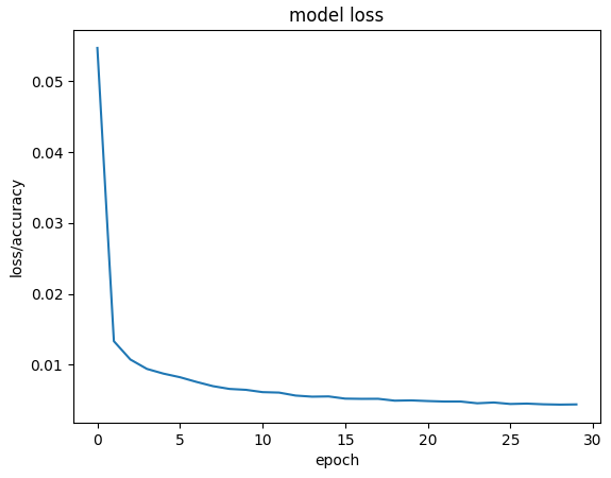
\includegraphics[width=0.7\linewidth]{gambar/bener/Loss_ModelCNN.png}
	\captionof{figure}{Loss Model CNN dengan epoch 30}
	\label{fig:lossModelCNN1}
\end{figure}
Gambar \ref{fig:lossModelCNN1}  menunjukkan perubahan \textit{loss} model selama proses pelatihan 30 siklus (iterasi pelatihan). Kerugian digunakan untuk mengukur seberapa baik prediksi model kita didasarkan pada nilai sebenarnya dari tugas regresi, atau untuk mengukur perbedaan antara prediksi model dan entri yang benar dalam tugas klasifikasi.

Pada awal pelatihan (Epoch 1) \textit{loss} memiliki nilai yang relatif tinggi yaitu sekitar 0,055. Hal ini menunjukkan bahwa model asli masih belum mampu membuat prediksi yang akurat.

Namun seiring dengan kemajuan jaman dan pendidikan, kerugian tersebut berangsur-angsur berkurang dari jaman ke jaman. Semakin kecil nilai kerugian, semakin baik model kita membuat prediksi yang mendekati nilai sebenarnya atau label yang benar.

Di akhir pelatihan (Epoch 30), kerugiannya sekitar 0,0044, menunjukkan bahwa model kami telah berhasil dipelajari dan mampu membuat prediksi yang cukup akurat. 

\begin{figure}[!hbt]
	\centering
	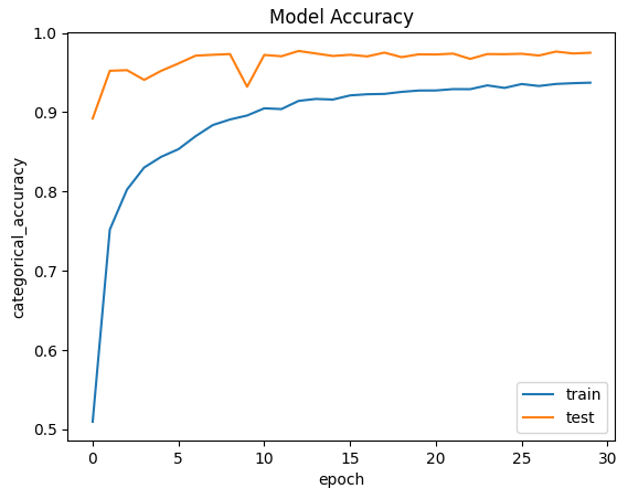
\includegraphics[width=0.7\linewidth]{gambar/bener/Accuracy_ModelCNN.png}
	\captionof{figure}{Akurasi Model CNN dengan epoch 30}
	\label{fig:AkurasiCNN1}
\end{figure}
Gambar \ref{fig:AkurasiCNN1} menunjukkan perubahan akurasi model dan akurasi validasi selama proses pelatihan dalam 30\textit{ epoch}

Pada awal pelatihan (epoch 1), akurasi model relatif rendah, sekitar 50,94\%, sedangkan akurasi validasi cukup tinggi, sekitar 89,20\%. Hal ini menunjukkan bahwa model masih perlu diperbaiki dari segi kemampuan prediksi data pelatihan.

Namun, seiring dengan kemajuan zaman dan kemajuan pendidikan, akurasi model secara bertahap meningkat dari zaman ke zaman. Akurasi konfirmasi juga meningkat dari waktu ke waktu. Pada akhir pelatihan (epoch 30), akurasi model sekitar 93,72\%, sedangkan akurasi validasi sekitar 97,50\%. Grafik ini menunjukkan peningkatan performa model yang berkelanjutan. Keakuratan data pelatihan dan validasi yang ditingkatkan berarti model kami belajar dengan sukses dan dapat menghasilkan prediksi yang lebih akurat dari waktu ke waktu.

Grafik ini menunjukkan peningkatan performa model yang berkelanjutan. Keakuratan data pelatihan dan validasi yang ditingkatkan berarti model kami belajar dengan sukses dan dapat menghasilkan prediksi yang lebih akurat dari waktu ke waktu.  

\begin{figure}[!hbt]
	\centering
	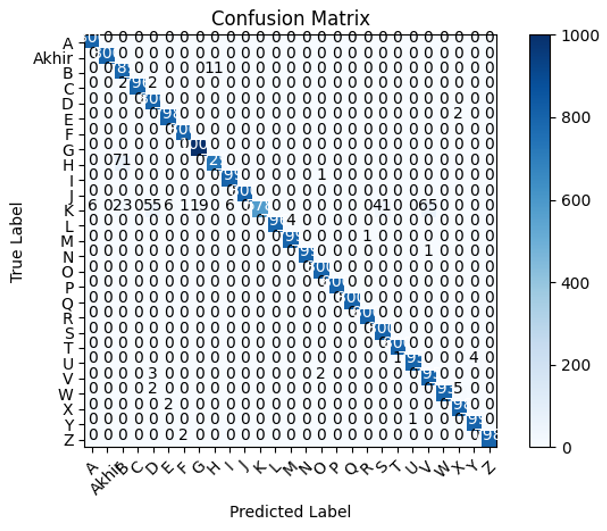
\includegraphics[width=0.7\linewidth]{gambar/bener/ConfusionMatrix_ModelCNN.png}
	\captionof{table}{Tabel Confusion Matriks Model CNN dengan epoch 30}
	\label{fig:TabelModelCNN1}
\end{figure}
Dalam kasus ini, matriks tersebut mencerminkan hasil dari deteksi huruf dalam suatu dataset. Terdapat 26 label huruf, yaitu A sampai Z. Diagonal utama dari matriks menunjukkan jumlah contoh yang diklasifikasikan dengan benar, di mana nilai-nilai tersebut merupakan \textit{True Positives } atau contoh yang benar-benar terdeteksi dengan benar untuk setiap huruf.

Berdasarkan Gambar \ref{fig:TabelModelCNN1}, ditemukan bahwa akurasi deteksi dan label huruf K sebesar 578. Hal ini disebabkan oleh kesalahan dalam dataset label huruf K yang terdapat 185 data pelatihan yang seharusnya berisi huruf V. Kesalahan ini terjadi karena kesalahan dalam pengelompokan data ke dalam folder yang menyebabkan kesalahan dalam mengidentifikasi huruf K sebagai huruf V. Dalam deteksi tersebut, terdapat 65 kasus di mana huruf K salah terdeteksi sebagai huruf V, 19 kasus sebagai huruf G, 23 kasus sebagai huruf B, dan 61 kasus sebagai huruf S.

Beberapa nilai di luar diagonal utama juga menunjukkan adanya kesalahan prediksi. Sebagai contoh, pada baris B dan kolom H terdapat 11 contoh yang seharusnya huruf B tetapi salah terklasifikasi sebagai huruf H \textit{False Positives}. Hal yang sama berlaku untuk kesalahan prediksi lainnya.

Berikut merupakan tabel perhitungan \textit{F1-score}, presisi, dan recall yang dapat dilihat pada Tabel \ref{tbl:TabelModelCNN} menggunakan \textit{Confusion Matrix} pada Gambar \ref{fig:TabelModelCNN1}

\begin{table}[!hbt]
	\centering
	\captionof{table}{Tabel Model CNN Confusion Matrix}
	\label{tbl:TabelModelCNN}
	\begin{tabular}{|c|c|c|c|c|}
	\hline
	Class & Precision & Recall & F1-score & Accuracy \\
	\hline
	A & 0.9926 & 1.0000 & 0.9963 & 1.0000 \\
	Akhir & 1.0000 & 1.0000 & 1.0000 & 1.0000 \\
	B & 0.8915 & 0.9863 & 0.9365 & 0.9863 \\
	C & 1.0000 & 0.9950 & 0.9975 & 0.9950 \\
	D & 0.9281 & 1.0000 & 0.9627 & 1.0000 \\
	E & 0.9901 & 0.9975 & 0.9938 & 0.9975 \\
	F & 0.9963 & 1.0000 & 0.9981 & 1.0000 \\
	G & 0.9814 & 1.0000 & 0.9906 & 1.0000 \\
	H & 0.9851 & 0.9113 & 0.9468 & 0.9113 \\
	I & 0.9925 & 0.9988 & 0.9956 & 0.9988 \\
	J & 1.0000 & 1.0000 & 1.0000 & 1.0000 \\
	K & 1.0000 & 0.7225 & 0.8389 & 0.7225 \\
	L & 1.0000 & 0.9950 & 0.9975 & 0.9950 \\
	M & 0.9950 & 0.9988 & 0.9969 & 0.9988 \\
	N & 1.0000 & 0.9988 & 0.9994 & 0.9988 \\
	O & 0.9963 & 1.0000 & 0.9981 & 1.0000 \\
	P & 1.0000 & 1.0000 & 1.0000 & 1.0000 \\
	Q & 1.0000 & 1.0000 & 1.0000 & 1.0000 \\
	R & 0.9988 & 1.0000 & 0.9994 & 1.0000 \\
	S & 0.9513 & 1.0000 & 0.9750 & 1.0000 \\
	T & 0.9988 & 1.0000 & 0.9994 & 1.0000 \\
	U & 0.9987 & 0.9938 & 0.9962 & 0.9938 \\
	V & 0.9233 & 0.9938 & 0.9573 & 0.9938 \\
	W & 1.0000 & 0.9913 & 0.9956 & 0.9913 \\
	X & 0.9913 & 0.9975 & 0.9944 & 0.9975 \\
	Y & 0.9950 & 0.9988 & 0.9969 & 0.9988 \\
	Z & 1.0000 & 0.9975 & 0.9987 & 0.9975 \\
	\hline
	\end{tabular}
\end{table}

Untuk rata-rata metrik evaluasi, Accuracy mencapai 98.94\%, Recall mencapai 99.75\%, \textit{Precision} mencapai 98.62\%, dan \textit{F1-score} mencapai 99.13\%. Hal ini menunjukkan bahwa secara keseluruhan, model CNN memiliki performa yang sangat baik dalam mengklasifikasikan huruf-huruf dalam dataset.


\section{Model CNN Kedua}
Pada Model CNN Kedua , Dataset tersebut melewati beberapa lapisan untuk mengekstraksi fitur. Pertama, dataset melewati lapisan \textit{Conv2D} dengan 32 \textit{neuron}, \textit{filter} 3x3, aktivasi \textit{ReLU}, dan \textit{padding} yang sama. Kemudian, dilakukan \textit{MaxPooling2D} dengan ukuran \textit{pooling} 2x2 dan \textit{padding} yang sama.

Selanjutnya, dataset melewati lapisan \textit{Conv2D} lain dengan 16 \textit{neuron}, \textit{filter} 3x3, aktivasi \textit{ReLU}, dan \textit{padding} yang sama sebanyak dua kali. Kemudian dilakukan lagi \textit{MaxPooling2D} dengan ukuran \textit{pooling} 2x2 dan \textit{padding} yang sama. Dan diakhiri dengan dataset melewati lapisan \textit{Conv2D} dengan 8 \textit{neuron} , \textit{filter} 3x3 , aktivasi \textit{ReLU} dan \textit{padding} yang sama sebanyak dua kali serta \textit{MaxPooling2D} dengan ukuran \textit{pooling} 2x2 

Setelah proses ekstraksi fitur, dataset kemudian masuk ke tahap klasifikasi. Pertama, dilakukan flattening untuk mengubah data menjadi vektor satu dimensi. Kemudian, data melewati lapisan \textit{Dense} dengan 16 \textit{neuron} dan aktivasi \textit{ReLU}. Untuk mencegah overfitting, dilakukan dropout dengan dropout rate 0.2. Setelah itu, terdapat lapisan \textit{Dense} lagi dengan 16 \textit{neuron} dan aktivasi \textit{ReLU}. Lapisan terakhir menggunakan \textit{Dense} dengan jumlah \textit{neuron} sesuai dengan jumlah kelas pada dataset (JumlahKelas) dan aktivasi \textit{softmax} untuk menghasilkan output probabilitas kelas. Model CNN ini menggunakan fungsi \textit{loss} \textit{mean squared error} dan optimizer \textit{Adam} dalam proses kompilasi

Grafik akurasi dari Model CNN Kedua tersedia di Gambar \ref{fig:AkurasiCNNKedua}. Dalam skenario ini, terdapat empat lapisan \textit{Conv2D} yang diikuti oleh \textit{Maxpooling}. Jumlah \textit{neuron} dalam setiap lapisan \textit{Conv2D} adalah 32, 16, 16, dan 8. Model CNN ini dilatih selama 30\textit{ epoch}.

Grafik \textit{loss} dari Model CNN Kedua dapat ditemukan di Gambar \ref{fig:lossModelCNNKedua}. \textit{Loss} function digunakan untuk mengukur sejauh mana prediksi model CNN mendekati nilai sebenarnya. Pada skenario ini, model CNN berhasil mengurangi \textit{loss} secara signifikan selama proses pelatihan selama 30\textit{ epoch}.

\begin{figure}[!hbt]
	\centering
	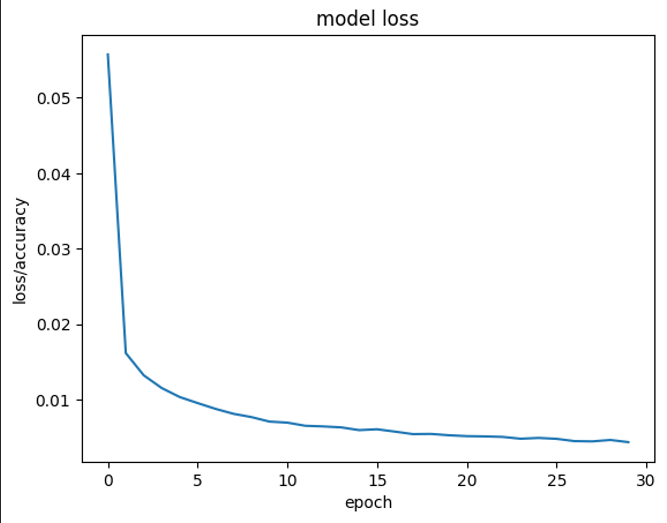
\includegraphics[width=0.7\linewidth]{gambar/bener/Loss_ModelCNN2.png}
	\captionof{figure}{Loss Model CNN 2 dengan epoch 30}
	\label{fig:lossModelCNNKedua}
\end{figure}

Seperti terlihat pada \ref{fig:lossModelCNNKedua}, \textit{loss} pada awal pelatihan (epoch 1) memiliki nilai yang relatif tinggi yaitu sekitar 0,056. Hal ini menunjukkan bahwa model asli masih belum mampu membuat prediksi yang akurat.

Namun seiring dengan kemajuan jaman dan pendidikan, kerugian tersebut berangsur-angsur berkurang dari jaman ke jaman. Semakin kecil nilai kerugian, semakin baik model kita membuat prediksi yang mendekati nilai sebenarnya atau label yang benar.

Di akhir pelatihan (epoch 30), \textit{loss} sekitar 0,00434, menunjukkan bahwa model kita telah berhasil dipelajari dan mampu membuat prediksi yang cukup akurat. Grafik ini menunjukkan proses pelatihan yang sukses, dengan kerugian terus menerus dan terus menurun dari musim ke musim. Ini menunjukkan bahwa model kami secara bertahap menangkap pola-pola penting dalam data dan meningkatkan prediktabilitas. 

\begin{figure}[!hbt]
	\centering
	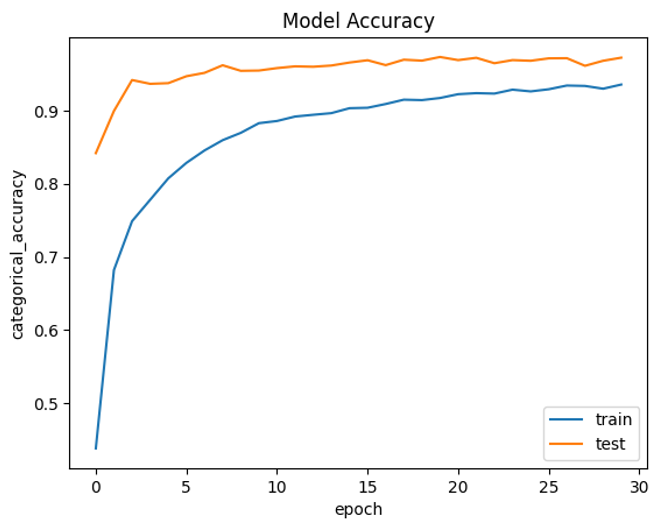
\includegraphics[width=0.7\linewidth]{gambar/bener/Accuracy_ModelCNN2.png}
	\captionof{figure}{Akurasi Model CNN 2 dengan epoch 30}
	\label{fig:AkurasiCNNKedua}
\end{figure}

Seperti terlihat pada Gambar \ref{fig:AkurasiCNNKedua}, akurasi model pada awal pelatihan (epoch 1) relatif rendah sekitar 43,85\%, sedangkan akurasi validasi cukup tinggi sekitar 84,17\%. Hal ini menunjukkan bahwa model asli masih perlu diperbaiki dalam hal kemampuan prediksi data pelatihan.

Namun, seiring dengan berjalannya\textit{ epoch} dan pelatihan, Akurasi model secara bertahap meningkat dari zaman ke zaman. Akurasi konfirmasi juga meningkat dari waktu ke waktu. Pada akhir pelatihan (epoch 30), akurasi model sekitar 93,53\%, sedangkan akurasi validasi sekitar 97,20\%. Gambar 10 menunjukkan peningkatan berkelanjutan dalam kinerja model. Keakuratan data pelatihan dan validasi yang lebih baik berarti bahwa model kami belajar dengan sukses dan dapat membuat prediksi yang lebih akurat dari waktu ke waktu. 	

\begin{figure}[!hbt]
	\centering
	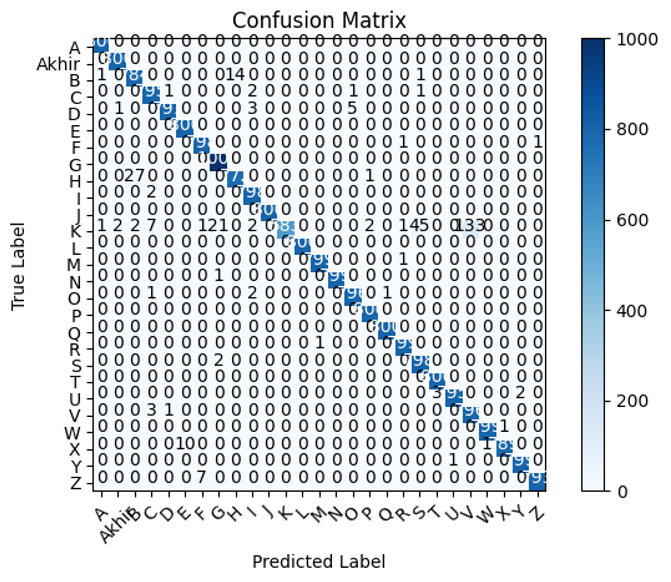
\includegraphics[width=0.7\linewidth]{gambar/bener/ConfusionMatrix_ModelCNN2.png}
	\captionof{table}{Tabel Confusion Matriks Model CNN Kedua dengan epoch 30}
	\label{fig:TabelModelCNNKedua}
\end{figure}
Berdasarkan Gambar \ref{fig:lossModelCNNKedua}, dapat dilihat bahwa dalam kasus deteksi dan label huruf K, terdapat akurasi sebesar 583. Hal ini disebabkan oleh adanya kesalahan dalam memasukkan dataset ke dalam folder training, sehingga dataset label huruf K sebenarnya juga mencakup huruf V. Sebagai akibatnya, model mengalami kesulitan dalam membedakan antara huruf K dan huruf V saat melakukan deteksi.

Dalam kasus ini, terdapat beberapa kesalahan deteksi yang menyebabkan nilai-nilai dalam \textit{Confusion Matrix} menjadi signifikan. Sebagai contoh, terdapat 7 kasus di mana huruf K salah terdeteksi sebagai huruf C, 21 kasus sebagai huruf G, 2 kasus sebagai huruf B, 2 kasus sebagai kata "Akhir", 45 kasus sebagai huruf S, dan 133 kasus sebagai huruf V. Kesalahan ini terjadi karena perbedaan bentuk dan fitur antara huruf K dan huruf V yang mungkin sulit untuk dikenali oleh model.

Berikut merupakan tabel perhitungan \textit{F1-score}, presisi, dan recall yang dapat dilihat pada Tabel \ref{tbl:ModelCNN2CONFUSIONMATRIX} menggunakan \textit{Confusion Matrix} pada Gambar \ref{fig:TabelModelCNNKedua}

\begin{center}
	\begin{table}[!hbt]
	\centering
	\captionof{table}{Tabel Model CNN 2 Confusion Matrix}
	\label{tbl:ModelCNN2CONFUSIONMATRIX}
	\begin{tabular}{|c|c|c|c|c|}
	\hline
	Class & Precision & Recall & F1-score & Accuracy \\
	\hline
	A & 0.9975 & 1.0000 & 0.9988 & 1.0000 \\
	Akhir & 0.9963 & 1.0000 & 0.9981 & 1.0000 \\
	B & 0.9643 & 0.9800 & 0.9721 & 0.9800 \\
	C & 0.9839 & 0.9938 & 0.9888 & 0.9938 \\
	D & 0.9975 & 0.9888 & 0.9931 & 0.9888 \\
	E & 0.9877 & 1.0000 & 0.9938 & 1.0000 \\
	F & 0.9901 & 0.9975 & 0.9938 & 0.9975 \\
	G & 0.9766 & 1.0000 & 0.9881 & 1.0000 \\
	H & 0.9822 & 0.9650 & 0.9735 & 0.9650 \\
	I & 0.9888 & 0.9975 & 0.9932 & 0.9975 \\
	J & 1.0000 & 1.0000 & 1.0000 & 1.0000 \\
	K & 1.0000 & 0.7288 & 0.8431 & 0.7288 \\
	L & 1.0000 & 1.0000 & 1.0000 & 1.0000 \\
	M & 0.9988 & 0.9988 & 0.9988 & 0.9988 \\
	N & 1.0000 & 0.9988 & 0.9994 & 0.9988 \\
	O & 0.9925 & 0.9950 & 0.9938 & 0.9950 \\
	P & 0.9963 & 1.0000 & 0.9981 & 1.0000 \\
	Q & 0.9988 & 1.0000 & 0.9994 & 1.0000 \\
	R & 0.9963 & 0.9988 & 0.9975 & 0.9988 \\
	S & 0.9444 & 0.9975 & 0.9702 & 0.9975 \\
	T & 0.9963 & 1.0000 & 0.9981 & 1.0000 \\
	U & 0.9987 & 0.9938 & 0.9962 & 0.9938 \\
	V & 0.8568 & 0.9950 & 0.9208 & 0.9950 \\
	W & 0.9988 & 0.9988 & 0.9988 & 0.9988 \\
	X & 0.9987 & 0.9863 & 0.9925 & 0.9863 \\
	Y & 0.9975 & 0.9988 & 0.9981 & 0.9988 \\
	Z & 0.9987 & 0.9913 & 0.9950 & 0.9913 \\
	\hline
	\end{tabular}
	\end{table}
\end{center}

Berdasarkan Tabel \ref{tbl:ModelCNN2CONFUSIONMATRIX}, model ini mencapai kinerja yang sangat memuaskan dalam mengklasifikasikan kelas yang berbeda. Model tersebut dapat mengidentifikasi berbagai kategori material dengan sangat tepat dengan akurasi 99,1\%. Skor F1 sebesar 99,3\% menunjukkan kemampuan model untuk memperhitungkan positif palsu dan negatif palsu. Tingkat pemulihan sebesar 99,8\% menunjukkan bahwa model tersebut memiliki tingkat keberhasilan yang tinggi dalam mengidentifikasi anggota yang positif. Selain itu, akurasi 98,9\% menunjukkan bahwa model mampu mengklasifikasikan elemen positif dari semua elemen positif dengan benar. 


\section{Model CNN ResNet50v2}
Pada Model CNN ResNet50v2, digunakan arsitektur \textit{ResNet50V2 }sebagai model dasar. \textit{ResNet50V2 }merupakan salah satu arsitektur jaringan saraf konvolusi yang terbukti efektif dalam pengenalan gambar.

\textit{ResNet50V2 }memiliki struktur yang dalam dengan total 50 lapisan. Arsitektur ini menggunakan blok residual untuk mengatasi masalah penurunan performa yang umum terjadi pada jaringan saraf konvolusi yang sangat dalam. Blok residual memanfaatkan koneksi lompatan (skip connection) untuk memperbaiki propagasi gradien, sehingga mengurangi penurunan performa saat jaringan semakin dalam . 

Selanjutnya , hasil keluaran dari model diambil dan diproses menggunakan operasi Global Average \textit{pooling} 2D untuk menghasilkan vektor fitur global dari seluruh gambar . Vektor fitur tersebut kemudian melewati lapisan \textit{Dense} dengan 16 \textit{neuron} dan aktivasi \textit{ReLU}. Untuk menghindari overfitting, dilakukan dropout dengan tingkat dropout sebesar 0.2. Kemudian, terdapat lapisan \textit{Dense} lain dengan 16 \textit{neuron} dan aktivasi \textit{ReLU}. Lapisan terakhir menggunakan \textit{Dense} dengan jumlah \textit{neuron} sesuai dengan jumlah kelas pada dataset (JumlahKelas) dan aktivasi \textit{softmax} untuk menghasilkan probabilitas kelas sebagai output . 

\subsection*{Performa dan Fungsionalitas Model CNN \textit{ResNet50v2 }Skenario Pertama}

Grafik akurasi dari Model CNN \textit{ResNet50V2 }tersedia pada Gambar \ref{fig:AkurasiCNNResNet50V2}. Pada skenario ini, model CNN menggunakan arsitektur \textit{ResNet50V2 }sebagai base model. Model CNN ini dilatih selama 30\textit{ epoch}.

Grafik \textit{loss} dari Model CNN \textit{ResNet50V2 }dapat dilihat pada Gambar \ref{fig:lossModelCNNResNet50v2}. \textit{Loss} function digunakan untuk mengukur sejauh mana prediksi model mendekati nilai sebenarnya. Pada skenario ini, model CNN berhasil mengurangi \textit{loss} secara signifikan selama proses pelatihan selama 30\textit{ epoch}.

\begin{figure}[!hbt]
	\centering
	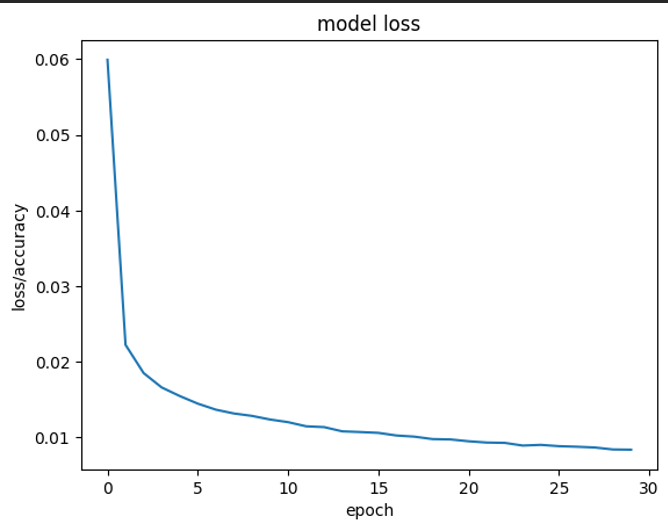
\includegraphics[width=0.7\linewidth]{gambar/bener/Loss_ModelCNNResNet50V2.png}
	\captionof{figure}{Loss Model CNN ResNet50V2 dengan epoch 30}
	\label{fig:lossModelCNNResNet50v2}
\end{figure}

Menurut Gambar\ref{fig:lossModelCNNResNet50v2}, kerugian awal pada awal pelatihan (epoch 1) cukup tinggi, sekitar 0,0599. Namun, seiring bertambahnya jumlah\textit{ epoch}, kerugian secara bertahap berkurang. Hal ini menunjukkan bahwa model secara perlahan mengoptimalkan parameternya untuk meminimalkan perbedaan antara keluaran yang diprediksi dan keluaran aktual.

Dengan setiap\textit{ epoch}, kerugian berkurang, menunjukkan bahwa model lebih baik dalam mempelajari pola dalam data pelatihan. Di musim terakhir (Epoch 30), kerugian berkurang menjadi sekitar 0,0084, menunjukkan bahwa model mencapai akurasi yang baik dalam memprediksi kelas yang benar. Pengurangan kerugian ini menunjukkan bahwa model CNN \textit{Xception} berhasil menghasilkan representasi fitur yang kuat dan mempelajari hubungan kompleks antara input gambar dan output kelas. Dengan kata lain, model ini mengenali pola pada gambar dan mengklasifikasikannya dengan akurasi tinggi.  
\begin{figure}[!hbt]
	\centering
	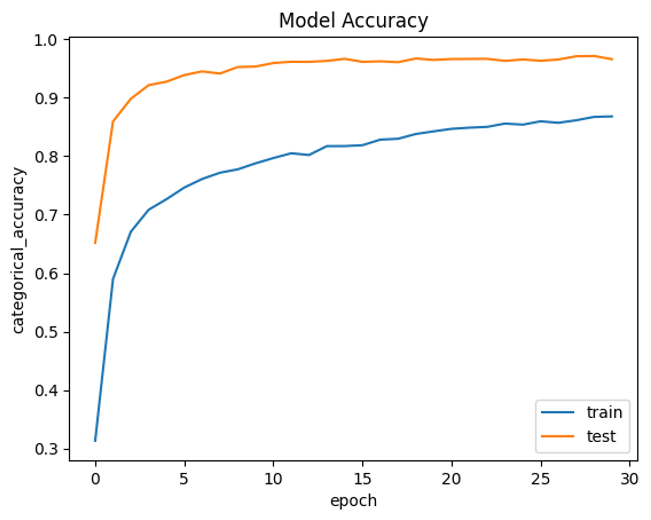
\includegraphics[width=0.7\linewidth]{gambar/bener/Accuracy_ModelResNet50V2.png}
	\captionof{figure}{Akurasi Model CNN ResNet50V2 dengan epoch 30}
	\label{fig:AkurasiCNNResNet50V2}
\end{figure}
Berdasarkan Gambar \ref{fig:AkurasiCNNResNet50V2}, pada awal pelatihan (epoch 1), tingkat akurasi awal rendah, sekitar 0,3134, dan tingkat akurasi validasi sekitar 0,6519. Namun, seiring bertambahnya jumlah\textit{ epoch}, keakuratan data pelatihan dan data validasi secara bertahap meningkat.

Akurasi meningkat pada setiap\textit{ epoch}, menunjukkan bahwa model semakin mampu mempelajari pola dari data pelatihan dan mentransfernya dengan baik ke data validasi. Pada\textit{ epoch} sebelumnya (epoch 30), akurasinya sekitar 86,8\% untuk data training dan 96,59\% untuk data validasi. Hal ini menunjukkan bahwa model mampu mengklasifikasikan citra dengan akurasi yang tinggi.  

\begin{figure}[!hbt]
	\centering
	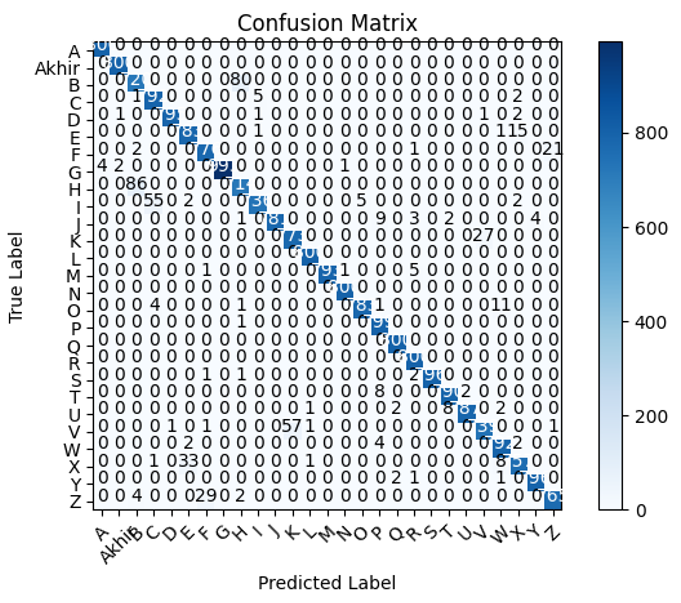
\includegraphics[width=0.7\linewidth]{gambar/bener/ConfusionMatrix_ModelCNNResNet50V2.png}
	\captionof{table}{Tabel Confusion Matriks Model CNN ResNet50V2 dengan epoch 30}
	\label{fig:TabelModelCNNResNet50v2}
\end{figure}
Dalam Tabel \textit{Confusion Matrix} sesuai \ref{fig:TabelModelCNNResNet50v2}, terdapat beberapa hasil yang perlu diperhatikan. Beberapa kelas huruf memiliki nilai \textit{True Poqsitives } yang tinggi, di mana huruf-huruf tersebut diklasifikasikan dengan benar oleh model. Contohnya, huruf A, Akhir, D, E, F, dan G memiliki \textit{True Positives} yang mendekati atau sama dengan 800, menunjukkan bahwa model berhasil mengklasifikasikan huruf-huruf tersebut dengan benar.

Namun, terdapat beberapa kesalahan dalam prediksi model. Sebagai contoh, pada baris B dan kolom H, terdapat 80 contoh yang seharusnya adalah huruf B tetapi salah terklasifikasi sebagai huruf H \textit{False Negatives} . Hal yang sama berlaku untuk kesalahan prediksi pada beberapa kelas huruf lainnya seperti C, I, J, S, U, dan V.

Beberapa nilai di luar diagonal utama juga menunjukkan adanya kesalahan prediksi. Misalnya, pada baris B dan kolom C terdapat 1 contoh yang seharusnya huruf B tetapi salah terklasifikasi sebagai huruf C \textit{False Positives}. Hal yang sama berlaku untuk kesalahan prediksi pada beberapa kelas huruf lainnya.

Matriks juga menunjukkan bahwa beberapa kelas huruf menghadapi kesulitan dalam pengklasifikasian. Sebagai contoh, pada baris K dan kolom K, terdapat 773 contoh yang berhasil diklasifikasikan dengan benar sebagai huruf K (True Positives), tetapi juga terdapat beberapa kesalahan dalam pengklasifikasian, seperti 27 contoh yang salah terklasifikasi sebagai huruf V \textit{False Positives}.

Berikut merupakan tabel perhitungan \textit{F1-score}, presisi, dan recall yang dapat dilihat pada Tabel \ref{tbl:Tabel Confusion Matrix ResNet50V2} menggunakan \textit{Confusion Matrix} pada Gambar \ref{fig:TabelModelCNNResNet50v2}

\begin{table}[!hbt]
	\centering
	\captionof{table}{Tabel Confusion Matrix ResNet50V2}
	\label{tbl:Tabel Confusion Matrix ResNet50V2}
	\begin{tabular}{|c|c|c|c|c|}
	\hline
	Class & Precision & Recall & F1-score & Accuracy \\
	\hline
	A & 0.9950 & 1.0000 & 0.9975 & 1.0000 \\
	Akhir & 0.9963 & 1.0000 & 0.9981 & 1.0000 \\
	B & 0.8856 & 0.9000 & 0.8927 & 0.9000 \\
	C & 0.9296 & 0.9900 & 0.9588 & 0.9900 \\
	D & 0.9987 & 0.9938 & 0.9962 & 0.9938 \\
	E & 0.9549 & 0.9788 & 0.9667 & 0.9788 \\
	F & 0.9604 & 0.9700 & 0.9652 & 0.9700 \\
	G & 1.0000 & 0.9930 & 0.9965 & 0.9930 \\
	H & 0.8925 & 0.8925 & 0.8925 & 0.8925 \\
	I & 0.9906 & 0.9200 & 0.9540 & 0.9200 \\
	J & 1.0000 & 0.9762 & 0.9880 & 0.9762 \\
	K & 0.9313 & 0.9662 & 0.9485 & 0.9662 \\
	L & 0.9963 & 1.0000 & 0.9981 & 1.0000 \\
	M & 1.0000 & 0.9912 & 0.9956 & 0.9912 \\
	N & 0.9975 & 1.0000 & 0.9988 & 1.0000 \\
	O & 0.9937 & 0.9788 & 0.9861 & 0.9788 \\
	P & 0.9732 & 0.9988 & 0.9858 & 0.9988 \\
	Q & 0.9950 & 1.0000 & 0.9975 & 1.0000 \\
	R & 0.9852 & 1.0000 & 0.9926 & 1.0000 \\
	S & 1.0000 & 0.9950 & 0.9975 & 0.9950 \\
	T & 0.9875 & 0.9875 & 0.9875 & 0.9875 \\
	U & 0.9975 & 0.9838 & 0.9906 & 0.9838 \\
	V & 0.9635 & 0.9238 & 0.9432 & 0.9238 \\
	W & 0.9718 & 0.9900 & 0.9808 & 0.9900 \\
	X & 0.9705 & 0.9463 & 0.9582 & 0.9463 \\
	Y & 0.9950 & 0.9950 & 0.9950 & 0.9950 \\
	Z & 0.9720 & 0.9563 & 0.9641 & 0.9563 \\
	\hline
	\end{tabular}
\end{table}

Secara umum sesuai \ref{tbl:Tabel Confusion Matrix ResNet50V2}, model ini tampil cukup baik dalam mengklasifikasikan kelas yang berbeda. Dalam hal presisi, model ini mencapai presisi rata-rata 99.04\%, menunjukkan tingkat keberhasilan yang baik dalam mengklasifikasikan data dengan benar. Rata-rata skor F1 sebesar 99.38\% menunjukkan kemampuan model untuk memperhitungkan positif palsu dan negatif palsu. Mengenai tingkat recall, model ini mencapai tingkat recall rata-rata 98.08\%, menunjukkan tingkat keberhasilan yang tinggi dalam mengidentifikasi anggota yang positif. Akurasi rata-rata 98.08\% menunjukkan kemampuan model untuk mengklasifikasikan elemen positif dari semua elemen positif dengan benar. 


\section{Model CNN Xception}
Pada Model ini digunakan sebuah model CNN berbasis arsitektur Xception. Arsitektur \textit{Xception} (Extreme Inception) adalah sebuah arsitektur jaringan saraf konvolusi yang dikembangkan oleh Francois Chollet. Arsitektur ini merupakan evolusi dari arsitektur Inception yang memperkenalkan konsep separable convolution.

Arsitektur \textit{Xception} memiliki struktur yang dalam dengan banyak lapisan konvolusi. Keunikan dari arsitektur ini terletak pada penggunaan operasi separable convolution, yang memisahkan operasi konvolusi menjadi dua tahap: konvolusi spasial dan konvolusi saluran. Hal ini memungkinkan pemodelan yang lebih efisien dan lebih akurat dalam mempelajari fitur-fitur dalam data gambar.

Pada model CNN yang diimplementasikan dalam Tugas Akhir ini, dimulai dengan mengambil input gambar dengan dimensi 128x128x3. Kemudian, model \textit{Xception} yang telah dilatih sebelumnya dengan menggunakan dataset ImageNet di-load sebagai model dasar. Lapisan-lapisan pada model dasar tersebut dibekukan (frozen) agar tidak mengalami perubahan bobot selama pelatihan model CNN ini.

Selanjutnya, output dari model dasar diambil dan melewati beberapa lapisan tambahan. Pertama, dilakukan operasi flatten untuk mengubah output menjadi vektor satu dimensi. Kemudian, terdapat dua lapisan \textit{Dense} dengan masing-masing 16 \textit{neuron} dan aktivasi \textit{ReLU}. Untuk mengurangi risiko overfitting, dilakukan dropout dengan tingkat dropout sebesar 0.2. Lapisan terakhir menggunakan \textit{Dense} dengan jumlah \textit{neuron} sesuai dengan jumlah kelas pada dataset (JumlahKelas) dan aktivasi \textit{softmax} untuk menghasilkan probabilitas kelas sebagai output.

Model CNN \textit{Xception} ini menggunakan fungsi \textit{loss} \textit{mean squared error} dan optimizer \textit{Adam} dalam proses kompilasi.

\subsection*{Performa dan Fungsionalitas Model CNN \textit{Xception} Skenario Pertama}

Grafik tingkat akurasi dari Model CNN \textit{Xception} dapat ditemukan pada Gambar \ref{fig:akurasiModelCNNXception}. Pada eksperimen ini, model CNN menggunakan arsitektur \textit{Xception} sebagai model dasar. Model CNN ini melalui proses pelatihan selama 30\textit{ epoch}.

Grafik tingkat kehilangan (loss) dari Model CNN \textit{Xception} tersedia pada Gambar \ref{fig:lossModelCNNXception}. \textit{Loss} function digunakan untuk mengukur seberapa dekat prediksi model dengan nilai sebenarnya. Dalam eksperimen ini, model CNN berhasil mengurangi tingkat kehilangan secara signifikan selama proses pelatihan selama 30\textit{ epoch}.

\begin{figure}[!hbt]
	\centering
	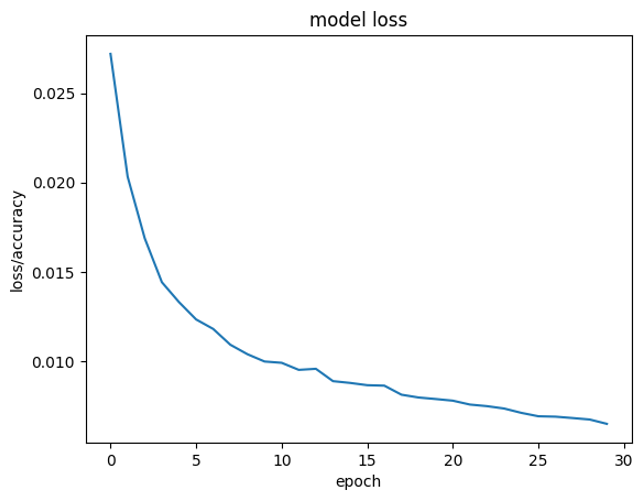
\includegraphics[width=0.7\linewidth]{gambar/bener/Loss_ModelXception.png}
	\captionof{figure}{\textit{Loss} Model CNN Xception dengan epoch 30}
	\label{fig:lossModelCNNXception}
\end{figure}

Berdasarkan Gambar \ref{fig:lossModelCNNXception}, nilai \textit{loss} pada awal pelatihan (epoch 1) cukup tinggi yaitu sekitar 0,027. Hal ini menunjukkan bahwa model asli tidak dapat memberikan prediksi yang akurat.

Namun, seiring dengan kemajuan zaman dan pendidikan, nilai \textit{loss} tersebut berangsur-angsur berkurang. Semakin kecil nilai \textit{loss}, semakin baik model mampu membuat prediksi yang mendekati nilai sebenarnya atau label yang benar.

Di akhir pelatihan (Epoch 30), nilai \textit{loss} sekitar 0,0065, menunjukkan bahwa model berhasil dipelajari dan dapat membuat prediksi yang cukup akurat.  

\begin{figure}[!hbt]
	\centering
	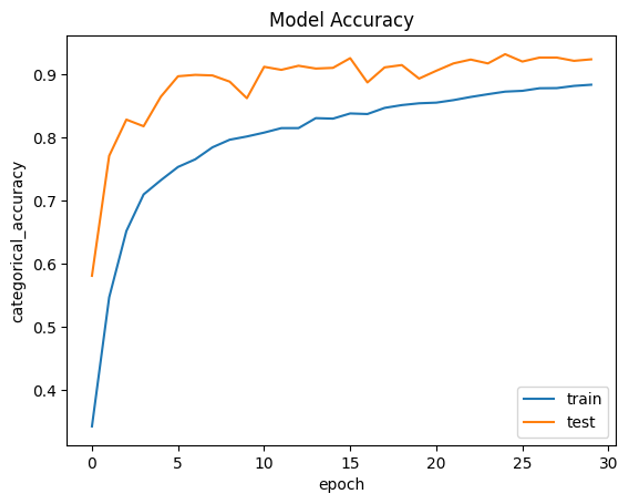
\includegraphics[width=0.7\linewidth]{gambar/bener/Accuracy_ModelXception.png}
	\captionof{figure}{Akurasi Model CNN Xception dengan epoch 30}
	\label{fig:akurasiModelCNNXception}
\end{figure}
Berdasarkan Gambar 14 , Pada awal pelatihan (Epoch 1), akurasi model relatif rendah, sekitar 34.20\%, sementara akurasi validasi sekitar 58.07\%. Ini menunjukkan bahwa model awal memiliki kinerja yang rendah dan perlu ditingkatkan.

Namun, seiring dengan berjalannya\textit{ epoch} dan pelatihan, akurasi model secara bertahap meningkat dari\textit{ epoch} ke\textit{ epoch}. Akurasi validasi juga mengalami peningkatan seiring waktu. Pada akhir pelatihan (Epoch 30), akurasi model mencapai sekitar 88.36\%, sedangkan akurasi validasi mencapai sekitar 92.39\%.

Grafik ini menggambarkan perbaikan performa model seiring berjalannya waktu. Terjadi peningkatan yang konsisten dalam akurasi model dan akurasi validasi dari\textit{ epoch} ke\textit{ epoch}.

Sebagai bagian dari pengujian fungsionalitas Model CNN Xception, dilakukan perhitungan \textit{Confusion Matrix} menggunakan dataset training sebanyak 21.600 data. \textit{Confusion Matrix} adalah sebuah matriks yang menampilkan jumlah data yang diklasifikasikan secara benar dan salah dalam setiap kelas. Detail dari \textit{Confusion Matrix} tersebut dapat ditemukan pada Gambar \ref{fig:TabelModelCNNResNet50v2}. Berdasarkan \textit{Confusion Matrix} yang dihasilkan, dilakukan perhitungan beberapa metrik evaluasi seperti \textit{F1-score}, presisi, dan \textit{recall}. Metrik-metrik evaluasi ini memberikan gambaran tentang performa dan akurasi Model CNN dalam melakukan klasifikasi.

\begin{figure}[!hbt]
	\centering
	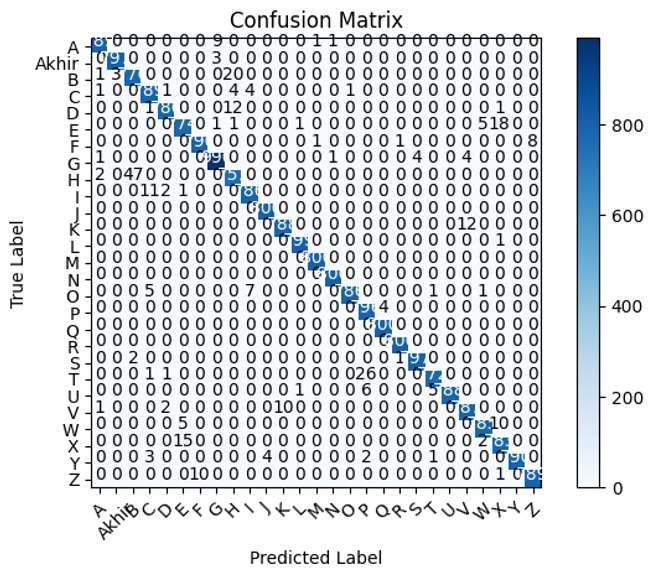
\includegraphics[width=0.7\linewidth]{gambar/bener/ConfusionMatrix_ModelXception.png}
	\captionof{figure}{Confusion Matrix Model CNN Xception dengan epoch 30}
	\label{fig:confusionmatrixModelCNNXception}
\end{figure}

Pada matriks tersebut, terdapat beberapa hasil yang perlu diperhatikan. Terlihat bahwa banyak kelas huruf yang berhasil diklasifikasikan dengan baik oleh model, seperti huruf A, Akhir, F, G, dan M, yang memiliki nilai \textit{True Positives } yang tinggi. Sebaliknya, terdapat beberapa kesalahan prediksi pada beberapa kelas huruf, seperti pada huruf B, C, D, E, H, dan I, yang memiliki beberapa False Positives dan False Negatives .

Dalam kasus ini, beberapa kelas huruf menghadapi kesulitan dalam pengklasifikasian. Sebagai contoh, huruf H dan I memiliki jumlah FP yang cukup signifikan, yang menunjukkan kesulitan model dalam membedakan antara kelas tersebut dengan kelas lainnya. Selain itu, huruf B juga mengalami kesulitan dalam pengklasifikasian, ditandai dengan jumlah FN dan FP yang lebih tinggi dibandingkan dengan kelas huruf lainnya.

Selain itu, terdapat pula beberapa kesalahan yang terjadi dalam prediksi. Misalnya, pada baris A dan kolom G, terdapat 9 contoh yang salah terklasifikasi sebagai huruf G, sedangkan pada baris G dan kolom A, terdapat 4 contoh yang salah terklasifikasi sebagai huruf A.

Berikut merupakan tabel perhitungan \textit{F1-score}, presisi, dan recall yang dapat dilihat pada Tabel \ref{tbl:Tabel Confusion Matrix Xception} \textit{Xception} menggunakan \textit{Confusion Matrix} pada Gambar \ref{fig:confusionmatrixModelCNNXception}.

\begin{center}
	\begin{table}[!hbt]
	\centering
	\captionof{table}{Tabel Confusion Matrix \textit{ Xception}}
	\label{tbl:Tabel Confusion Matrix Xception}
	\begin{tabular}{|c|c|c|c|c|}
	\hline
	Class & Precision & Recall & F1-score & Accuracy \\
	\hline
	A & 0.9925 & 0.9863 & 0.9893 & 0.9863 \\
	Akhir & 0.9963 & 0.9963 & 0.9963 & 0.9963 \\
	B & 0.9406 & 0.9700 & 0.9551 & 0.9700 \\
	C & 0.9741 & 0.9863 & 0.9801 & 0.9863 \\
	D & 0.9924 & 0.9825 & 0.9874 & 0.9825 \\
	E & 0.9736 & 0.9675 & 0.9705 & 0.9675 \\
	F & 0.9875 & 0.9875 & 0.9875 & 0.9875 \\
	G & 0.9870 & 0.9900 & 0.9885 & 0.9900 \\
	H & 0.9530 & 0.9388 & 0.9458 & 0.9388 \\
	I & 0.9862 & 0.9825 & 0.9843 & 0.9825 \\
	J & 0.9950 & 1.0000 & 0.9975 & 1.0000 \\
	K & 0.9875 & 0.9850 & 0.9862 & 0.9850 \\
	L & 0.9975 & 0.9988 & 0.9981 & 0.9988 \\
	M & 0.9975 & 1.0000 & 0.9988 & 1.0000 \\
	N & 0.9975 & 1.0000 & 0.9988 & 1.0000 \\
	O & 0.9987 & 0.9825 & 0.9905 & 0.9825 \\
	P & 0.9590 & 0.9950 & 0.9767 & 0.9950 \\
	Q & 0.9950 & 1.0000 & 0.9975 & 1.0000 \\
	R & 0.9975 & 1.0000 & 0.9988 & 1.0000 \\
	S & 0.9950 & 0.9963 & 0.9956 & 0.9963 \\
	T & 0.9910 & 0.9650 & 0.9778 & 0.9650 \\
	U & 1.0000 & 0.9850 & 0.9924 & 0.9850 \\
	V & 0.9801 & 0.9838 & 0.9819 & 0.9838 \\
	W & 0.9899 & 0.9813 & 0.9856 & 0.9813 \\
	X & 0.9619 & 0.9788 & 0.9703 & 0.9788 \\
	Y & 1.0000 & 0.9875 & 0.9937 & 0.9875 \\
	Z & 0.9900 & 0.9863 & 0.9881 & 0.9863 \\
	\hline
	\end{tabular}
\end{table}
\end{center}

Berdasarkan \ref{tbl:Tabel Confusion Matrix Xception} , Rata-rata \textit{Precision}, Recall, \textit{F1-Score}, dan \textit{Accuracy} dari model CNN yang dihasilkan dapat memberikan gambaran tentang kinerja keseluruhan model dalam mengklasifikasikan huruf dan kata yang diuji. Dari analisis tabel, ditemukan bahwa rata-rata \textit{Precision} sebesar 98.77\%, yang menunjukkan bahwa model memiliki kemampuan yang baik dalam mengidentifikasi kelas dengan benar. Selain itu, rata-rata Recall sebesar 98.72\% mengindikasikan kemampuan model dalam menemukan kembali sampel positif dari suatu kelas. Rata-rata \textit{F1-Score} sebesar 98.73\% menggambarkan keseimbangan antara \textit{Precision} dan Recall, menghasilkan pengukuran keseluruhan yang baik. Terakhir, rata-rata \textit{Accuracy} sebesar 98.78\% menunjukkan tingkat keseluruhan ketepatan model dalam mengklasifikasikan keseluruhan sampel dengan benar.


\section{Hasil Waktu Pelatihan}
Selain mendapatkan nilai akurasi , \textit{loss} , tabel \textit{Confusion Matrix} , \textit{F1-Score} , Recall maupun Presisi . Di dalam penelitian ini juga didapatkan hasil dari lama waktu selama melakukan pelatihan model berbagai macam skenario dari setiap \textit{ epoch} yang berhasil dilewati 

Berikut ini merupakan tabel yang memaparkan informasi terkait lama waktu pelatihan model per\textit{ epoch} dari masing-masing skenario yang telah diujicoba 

\begin{table}[!hbt]
	\centering
	\captionof{table}{Durasi Pelatihan dalam detik untuk Epoch 1-30}
	\label{tab:training_time}
	\begin{tabular}{|c|c|c|c|c|} 
	\hline
	Epoch & CNN & CNN2 & Xception & ResNet50V2\\
	\hline
	1              & 18.89        & 19.64         & 212.01            & 200.52              \\
	2              & 19.14        & 19.39         & 204.80            & 208.99              \\
	3              & 18.99        & 18.83         & 210.35            & 201.25              \\
	4              & 18.86        & 19.78         & 214.80            & 191.17              \\
	5              & 19.14        & 20.40         & 201.79            & 195.61              \\
	6              & 20.20        & 20.12         & 202.45            & 192.91              \\
	7              & 19.83        & 19.97         & 198.41            & 192.96              \\
	8              & 21.73        & 19.28         & 192.45            & 191.49              \\
	9              & 20.27        & 20.17         & 189.75            & 196.54              \\
	10             & 19.94        & 20.77         & 188.84            & 199.96              \\
	11             & 20.97        & 21.56         & 189.66            & 195.11              \\
	12             & 21.17        & 20.56         & 187.79            & 188.70              \\
	13             & 21.55        & 20.19         & 188.07            & 189.04              \\
	14             & 21.36        & 20.55         & 185.68            & 224.72              \\
	15             & 21.19        & 19.37         & 184.83            & 208.74              \\
	16             & 21.02        & 20.11         & 185.04            & 217.11              \\
	17             & 21.24        & 20.80         & 188.87            & 204.28              \\
	18             & 21.51        & 19.41         & 190.76            & 224.57              \\
	19             & 21.45        & 19.78         & 193.68            & 204.64              \\
	20             & 21.79        & 19.77         & 193.92            & 181.35              \\
	21             & 20.57        & 19.80         & 186.56            & 175.74              \\
	22             & 21.11        & 20.40         & 185.24            & 180.82              \\
	23             & 21.48        & 20.14         & 185.09            & 173.18              \\
	24             & 21.00        & 20.09         & 186.67            & 163.73              \\
	25             & 21.90        & 20.12         & 185.66            & 168.90              \\
	26             & 23.09        & 20.31         & 185.45            & 164.35              \\
	27             & 22.81        & 19.69         & 184.81            & 164.39              \\
	28             & 23.44        & 19.10         & 185.45            & 163.14              \\
	29             & 22.45        & 19.27         & 187.25            & 161.36              \\
	30             & 22.35        & 19.54         & 187.09            & 162.61              \\ 
	\hline
	\end{tabular}
\end{table}

Berdasarkan tabel di atas, dapat dilihat bahwa Model CNN memiliki waktu pelatihan yang relatif stabil selama 30\textit{ epoch}, dengan rata-rata waktu pelatihan sekitar 19-22 detik per\textit{ epoch}. Model CNN2 juga memiliki pola waktu pelatihan yang serupa, dengan rata-rata waktu pelatihan sekitar 19-21 detik per\textit{ epoch}.

Di sisi lain, Model \textit{Xception} dan Model \textit{ResNet50V2 }memiliki waktu pelatihan yang lebih lama secara signifikan. Model \textit{Xception} membutuhkan waktu pelatihan sekitar 185-213 detik per\textit{ epoch}, sementara Model \textit{ResNet50V2 }membutuhkan waktu pelatihan sekitar 163-225 detik per\textit{ epoch}.
	
Dapat disimpulkan bahwa Model CNN dan Model CNN2 memiliki waktu pelatihan yang lebih efisien dibandingkan dengan Model \textit{Xception} dan Model ResNet50V2. Ini mungkin dikaitkan dengan perbedaan arsitektur dan kompleksitas model tersebut. Model CNN dan CNN2 mungkin lebih sederhana dan memiliki jumlah parameter yang lebih sedikit dibandingkan dengan \textit{Xception} dan ResNet50V2, sehingga memungkinkan pelatihan yang lebih cepat.

\section{Ujicoba Deteksi}
Dalam bagian ini , Telah dilakukan ujicoba perangkat lunak yang sudah dibuat dengan cara melakukan ujicoba langsung kepada orang yang mencoba . Dalam ujicoba kali ini diberikan contoh deteksi huruf vokal yaitu A,I,U,E,O dan membentuk kata seperti Bapak , Ibu dan Tante . Ujicoba ini dilakukan terhadap dua orang dengan mengambil jarak 100 cm dari Kamera

\subsection{Orang Pertama}
Pada tahap ujicoba ini, telah dilakukan serangkaian percobaan menggunakan beberapa model CNN yang berbeda, yaitu Model CNN, Model CNN2, Model CNN ResNet50V2, dan Model CNN Xception. Ujicoba tersebut bertujuan untuk menguji kemampuan dan kinerja masing-masing model dalam mengenali huruf serta merangkainya menjadi kata-kata. Dalam setiap percobaan, orang pertama telah menjadi subjek yang diuji dengan menggunakan model-model tersebut. 

Hasil ujicoba akan memberikan pemahaman yang lebih mendalam tentang keefektifan dan kehandalan masing-masing model dalam mengenali dan mengolah huruf-huruf menjadi kata-kata 

\subsubsection*{Hasil Model CNN Orang Pertama}

Setelah melalui serangkaian ujicoba, ModelCNN telah menunjukkan kinerjanya yang luar biasa dalam melakukan deteksi huruf dengan tingkat keberhasilan yang sangat baik. Salah satu kemampuan utamanya adalah mampu mengenali huruf-huruf dengan akurasi yang tinggi, bahkan dalam berbagai posisi dan pose yang berbeda

\begin{table}[!hbt]
	\centering
	\captionof{table}{Tabel Contoh Huruf/Kata dan Gambar Pose Model CNN Orang Pertama}
	\label{tbl:Tabel Contoh Huruf/Kata dan Gambar Pose Model CNN Orang Pertama}
	\begin{tabular}{|c|c|c|}
	\hline
	No & Huruf/Kata & Gambar Pose Model CNN \\
	\hline
	1 & A & 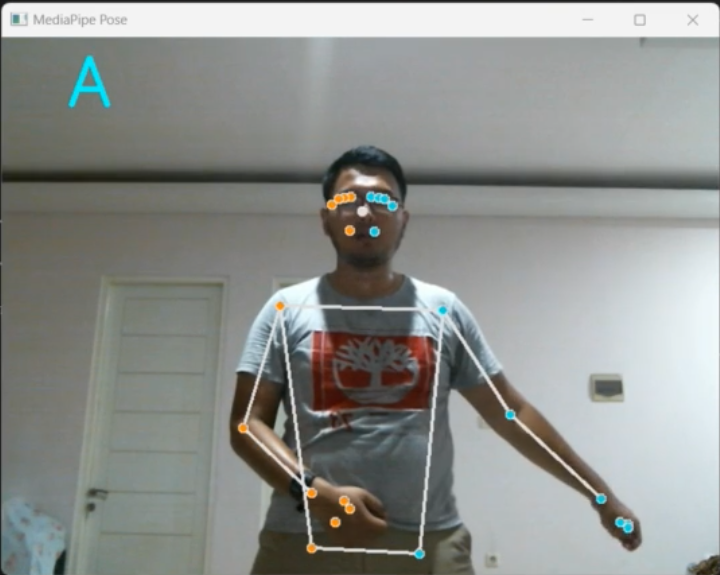
\includegraphics[width=0.2\textwidth]{gambar/bener/HurufA_ModelCNN_Dawe.png} \\
	\hline
	2 & I & 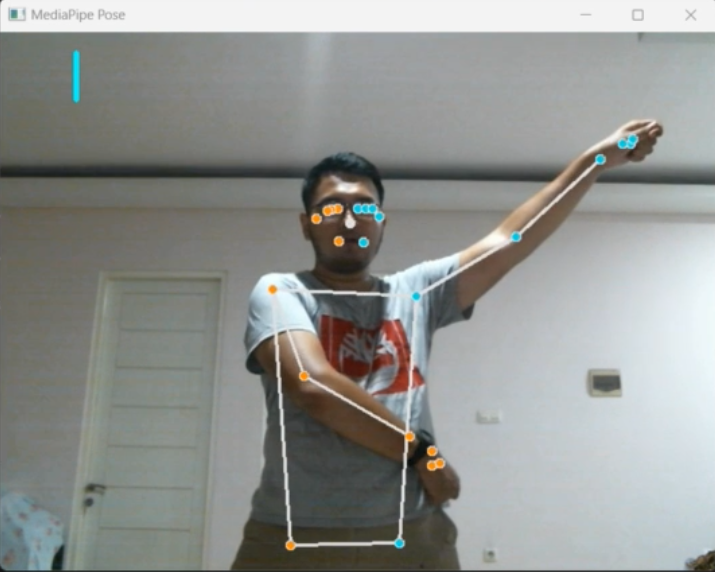
\includegraphics[width=0.2\textwidth]{gambar/bener/HurufI_ModelCNN_Dawe.png} \\
	\hline
	3 & U & 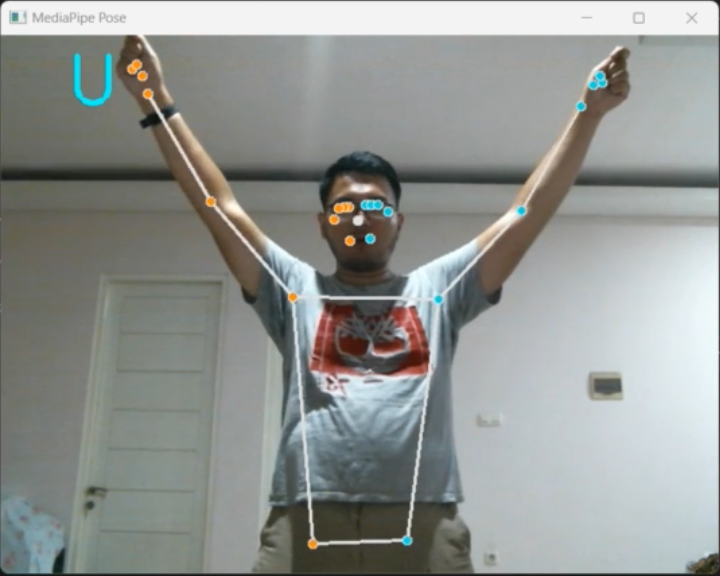
\includegraphics[width=0.2\textwidth]{gambar/bener/HurufU_ModelCNN_Dawe.png} \\
	\hline
	4 & E & 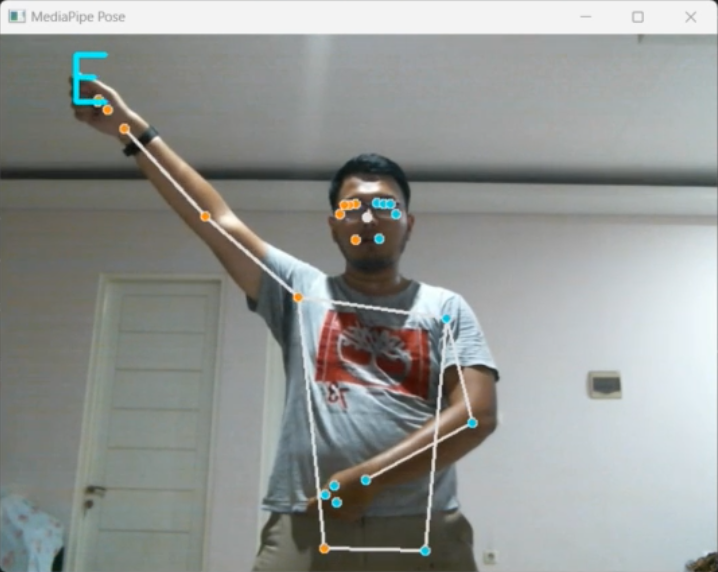
\includegraphics[width=0.2\textwidth]{gambar/bener/HurufE_ModelCNN_Dawe.png} \\
	\hline
	5 & O & 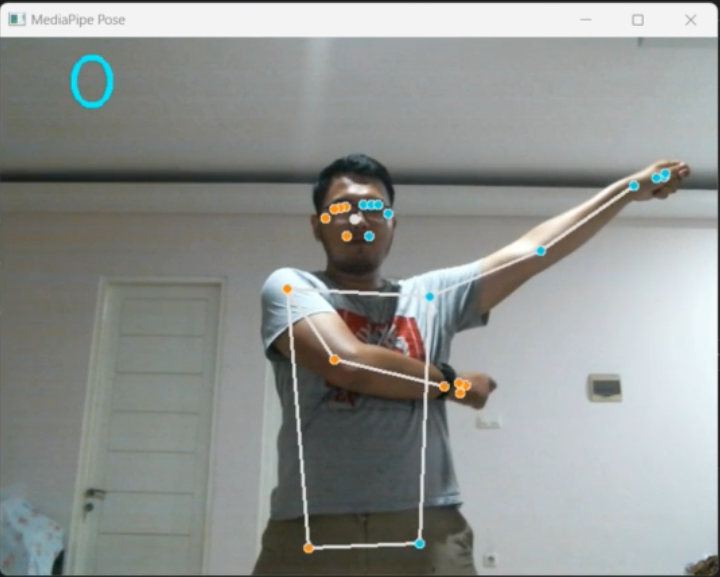
\includegraphics[width=0.2\textwidth]{gambar/bener/HurufO_ModelCNN_Dawe.png} \\
	\hline
	6 & B & 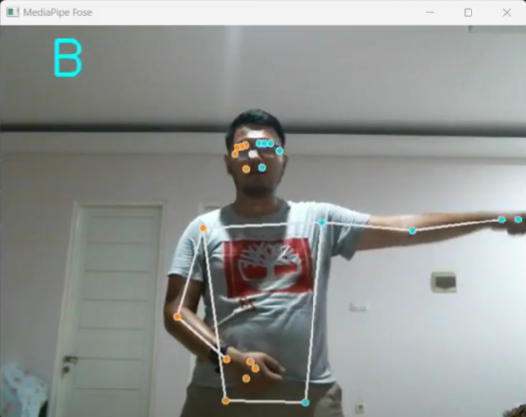
\includegraphics[width=0.2\textwidth]{gambar/bener/HurufB_ModelCNN_Dawe.png} \\
	\hline
	7 & K & 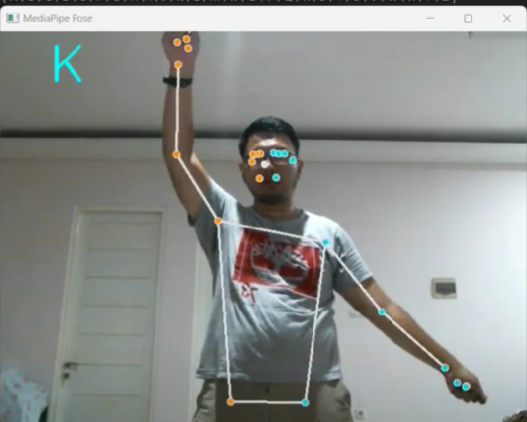
\includegraphics[width=0.2\textwidth]{gambar/bener/HurufK_ModelCNN_Dawe.png} \\
	\hline
	8 & H & 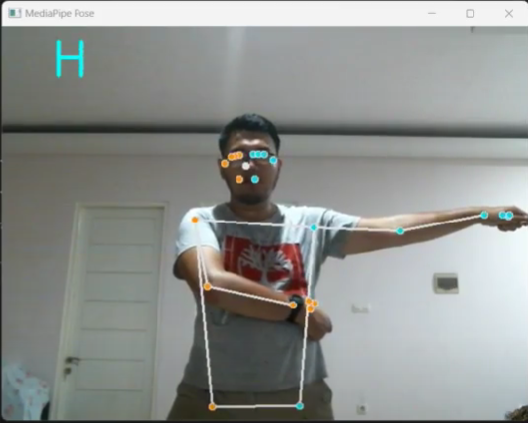
\includegraphics[width=0.2\textwidth]{gambar/bener/HurufH_ModelCNN_Dawe.png} \\
	\hline
	% Lanjutkan baris tabel sesuai kebutuhan
	\end{tabular}
\end{table}

\begin{table}[!hbt]
	\centering
	\captionof{table}{Tabel Contoh Huruf/Kata dan Gambar Pose Model CNN Orang Pertama}
	\begin{tabular}{|c|c|c|}
		\hline
		No & Huruf/Kata & Gambar Pose Model  \\
		\hline
		9 & Bapak & 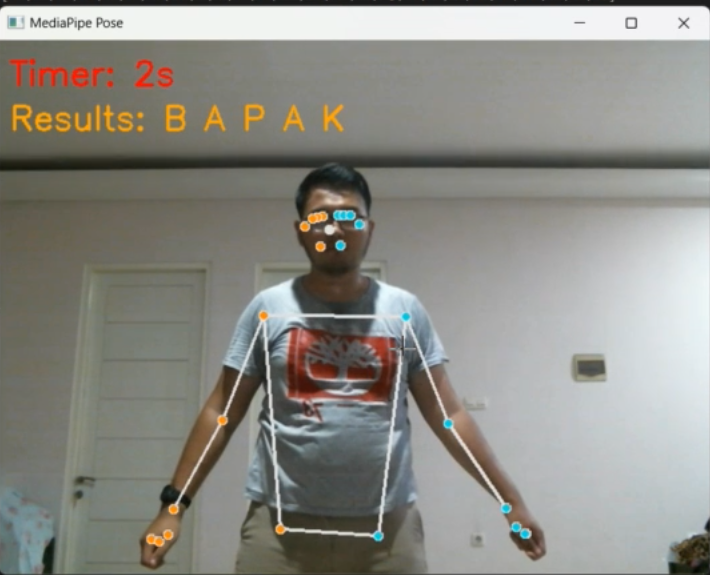
\includegraphics[width=0.2\textwidth]{gambar/bener/HurufBapak_ModelCNN_Dawe.png} \\
		\hline
		10 & Ibu & 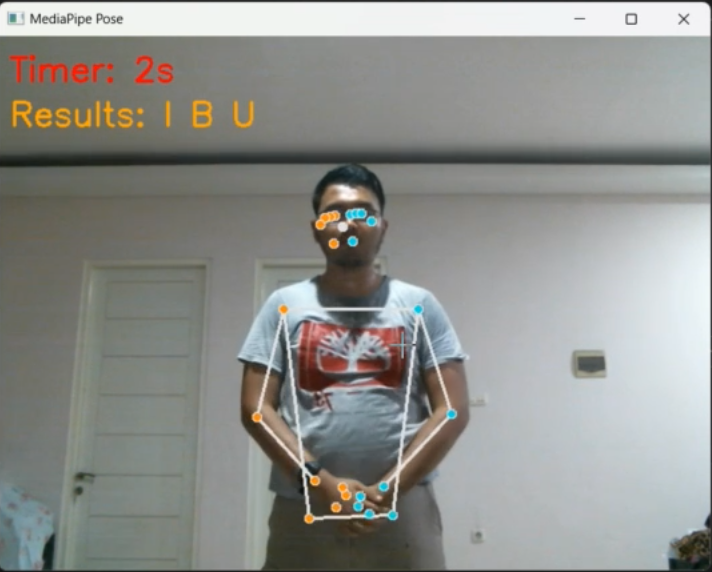
\includegraphics[width=0.2\textwidth]{gambar/bener/HurufIbu_ModelCNN_Dawe.png} \\
		\hline
		11 & Tante & 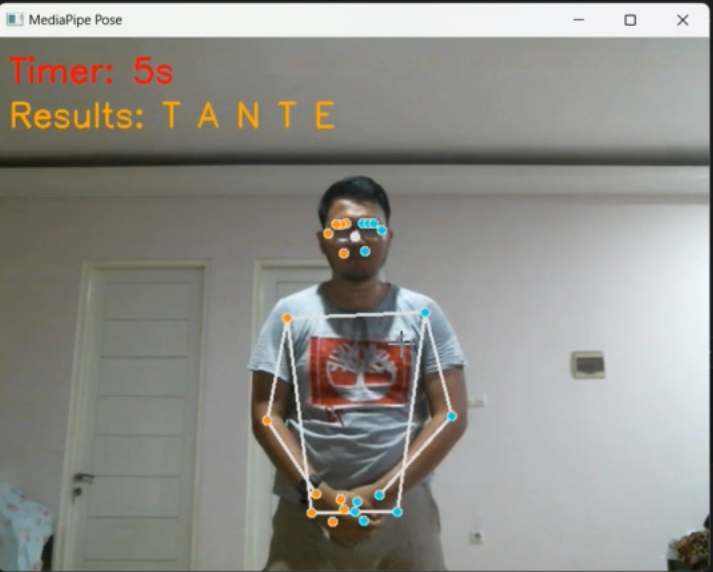
\includegraphics[width=0.2\textwidth]{gambar/bener/HurufTante_ModelCNN_Dawe.png} \\
		\hline
	\end{tabular}
\end{table}

\subsubsection*{Hasil Model CNN2 Orang Pertama}

Dari hasil ujicoba yang dilakukan, ModelCNN2 telah berhasil dalam melakukan deteksi dengan tingkat keberhasilan yang baik. Salah satu kemampuan utama model ini adalah mampu mendeteksi huruf-huruf dengan akurasi yang tinggi

\begin{table}[!hbt]
	\centering
	\captionof{table}{Tabel Contoh Huruf/Kata dan Gambar Pose Model CNN2 Orang Pertama}
	\label{tbl:Tabel Contoh Huruf/Kata dan Gambar Pose Model CNN2 Orang Pertama}
	\begin{tabular}{|c|c|c|}
	\hline
	No & Huruf/Kata & Gambar Pose Model  \\
	\hline
	1 & A & 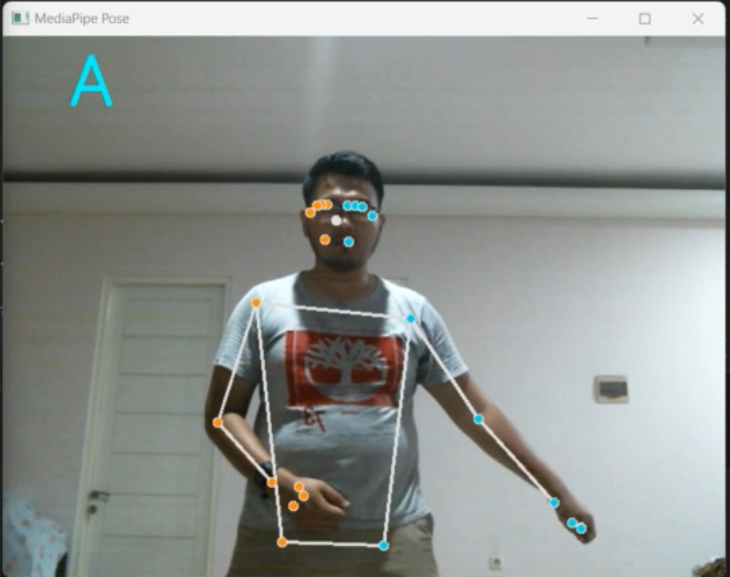
\includegraphics[width=0.2\textwidth]{gambar/bener/HurufA_ModelCNN2_Dawe.png} \\
	\hline
	2 & I & 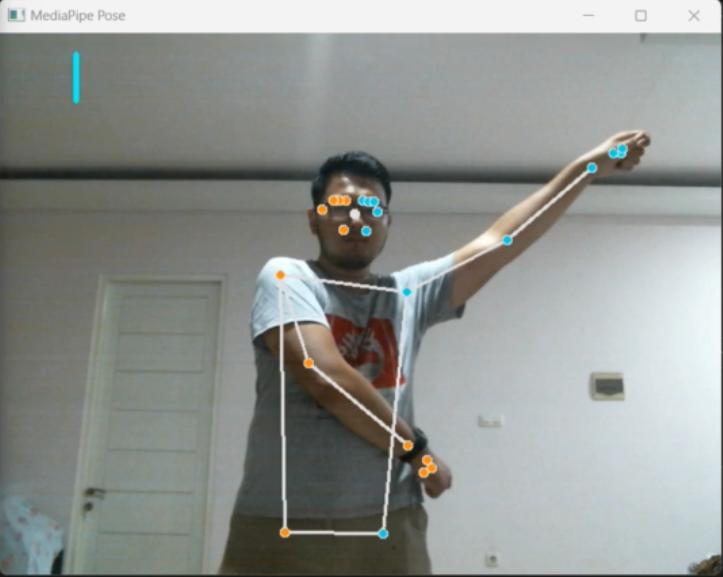
\includegraphics[width=0.2\textwidth]{gambar/bener/HurufI_ModelCNN2_Dawe.png} \\
	\hline
	3 & U & 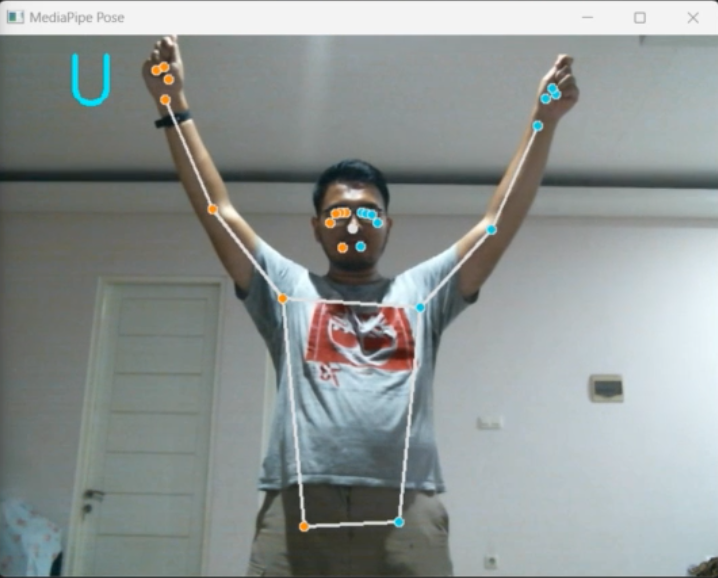
\includegraphics[width=0.2\textwidth]{gambar/bener/HurufU_ModelCNN2_Dawe.png} \\
	\hline
	4 & E & 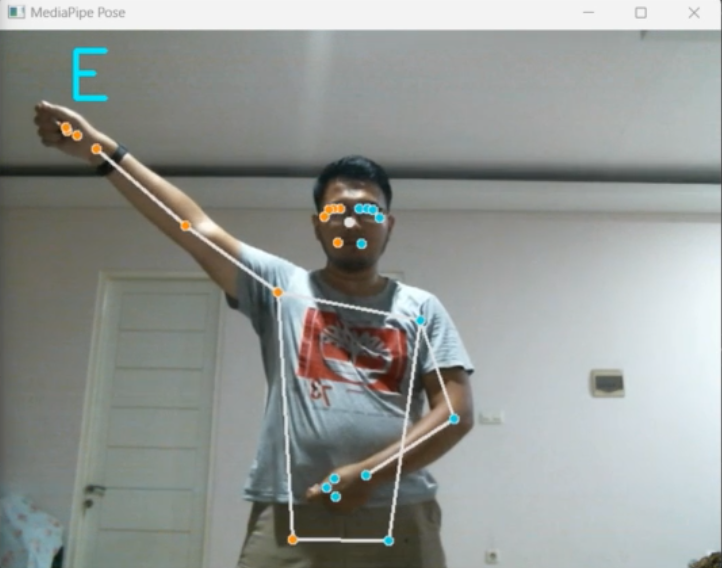
\includegraphics[width=0.2\textwidth]{gambar/bener/HurufE_ModelCNN2_Dawe.png} \\
	\hline
	5 & O & 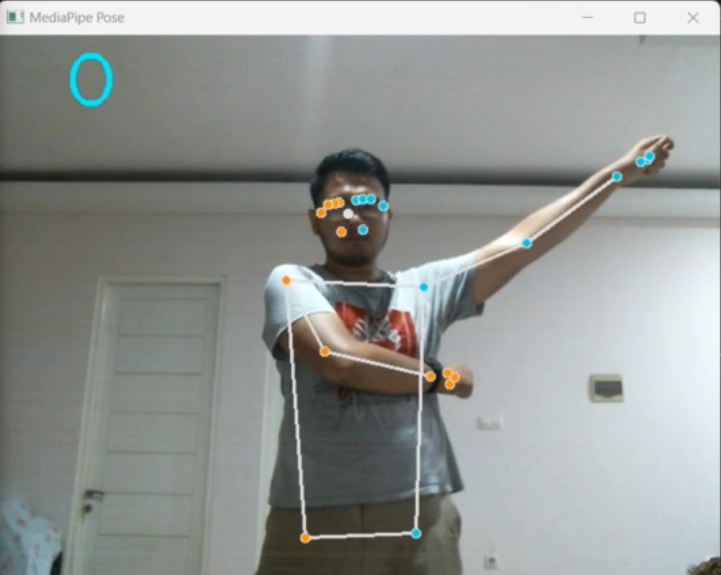
\includegraphics[width=0.2\textwidth]{gambar/bener/HurufO_ModelCNN2_Dawe.png} \\
	\hline
	6 & B & 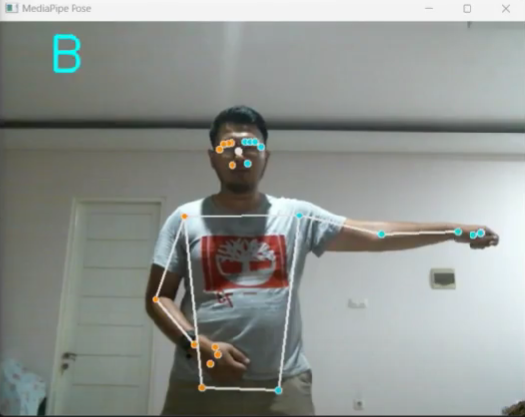
\includegraphics[width=0.2\textwidth]{gambar/bener/HurufB_ModelCNN2_Dawe.png} \\
	\hline
	7 & K & 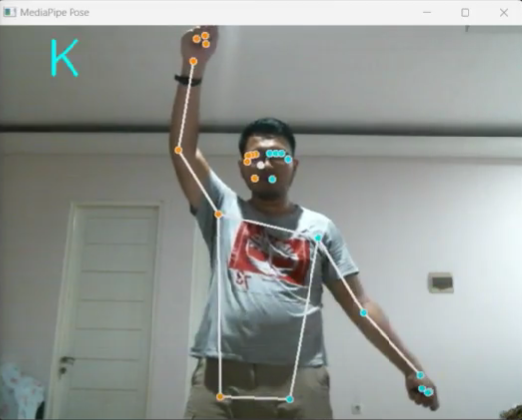
\includegraphics[width=0.2\textwidth]{gambar/bener/HurufK_ModelCNN2_Dawe.png} \\
	\hline
	8 & H & 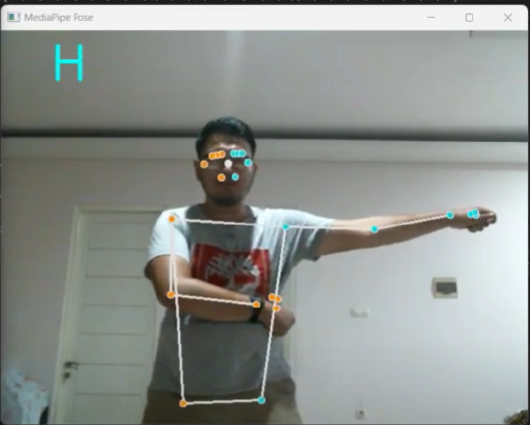
\includegraphics[width=0.2\textwidth]{gambar/bener/HurufH_ModelCNN2_Dawe.png} \\
	\hline
	% Lanjutkan baris tabel sesuai kebutuhan
	\end{tabular}
\end{table}

\begin{table}[!hbt]
	\centering
	\captionof{table}{Tabel Contoh Huruf/Kata dan Gambar Pose Model CNN2 Orang Pertama}
	\begin{tabular}{|c|c|c|}
		\hline
		No & Huruf/Kata & Gambar Pose Model  \\
		\hline
		9 & Bapak & 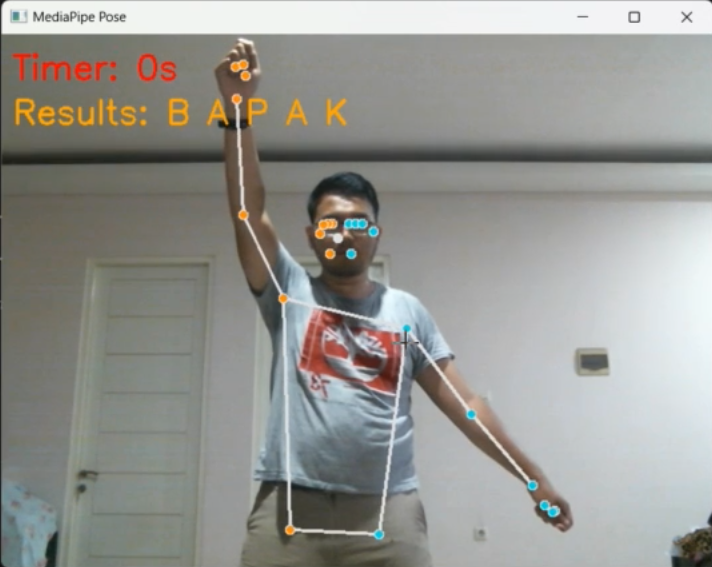
\includegraphics[width=0.2\textwidth]{gambar/bener/HurufBapak_CNN2_Dawe.png} \\
		\hline
		10 & Ibu & 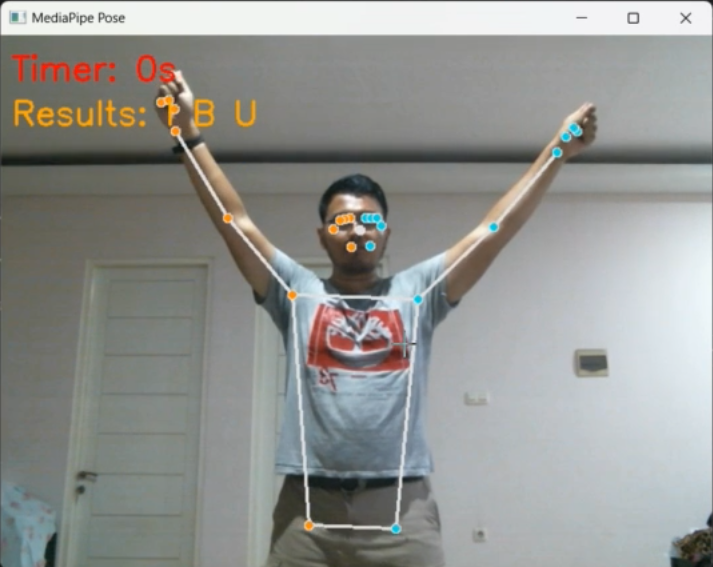
\includegraphics[width=0.2\textwidth]{gambar/bener/HurufIbu_ModelCNN2_Dawe.png} \\
		\hline
		11 & Tante & 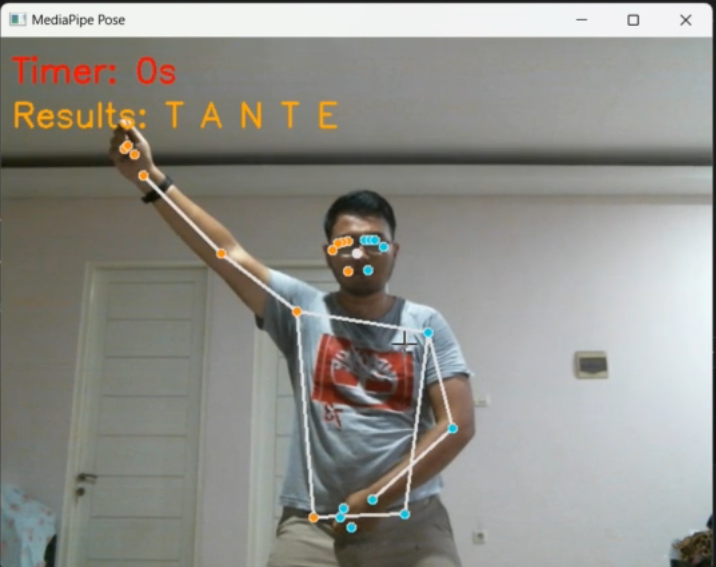
\includegraphics[width=0.2\textwidth]{gambar/bener/HurufTante_ModelCNN2_Dawe.png} \\
		\hline
	\end{tabular}
\end{table}

\subsubsection*{Hasil Model CNN \textit{ResNet50V2 }Orang Pertama}

Berdasarkan hasil ujicoba yang dilakukan, ModelCNN \textit{ResNet50V2 }telah menunjukkan kemampuannya yang sangat baik dalam melakukan deteksi huruf dengan tingkat keberhasilan yang tinggi. Salah satu keunggulan utama dari model ini adalah kemampuannya untuk mendeteksi huruf dengan akurat, bahkan dalam pose yang bervariasi. Dalam ujicoba tersebut, ModelCNN \textit{ResNet50V2 }berhasil mengatasi tantangan yang mungkin muncul akibat perubahan pose huruf, sehingga dapat mengenali huruf-huruf dengan presisi yang memuaskan

\begin{table}[!hbt]
	\centering
	\captionof{table}{Tabel Contoh Huruf/Kata dan Gambar Pose Model CNN \textit{ResNet50V2 }Orang Pertama}
	\label{tbl:Tabel Contoh Huruf/Kata dan Gambar Pose Model CNN ResNet50V2 Orang Pertama}
	\begin{tabular}{|c|c|c|}
	\hline
	No & Huruf/Kata & Gambar Pose Model  \\
	\hline
	1 & A & 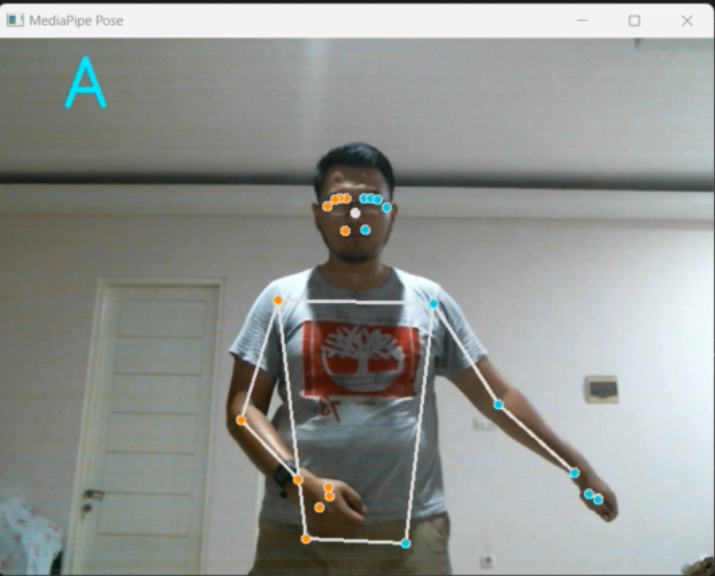
\includegraphics[width=0.2\textwidth]{gambar/bener/HurufA_ModelCNNResNet50V2_Dawe.png} \\
	\hline
	2 & I & 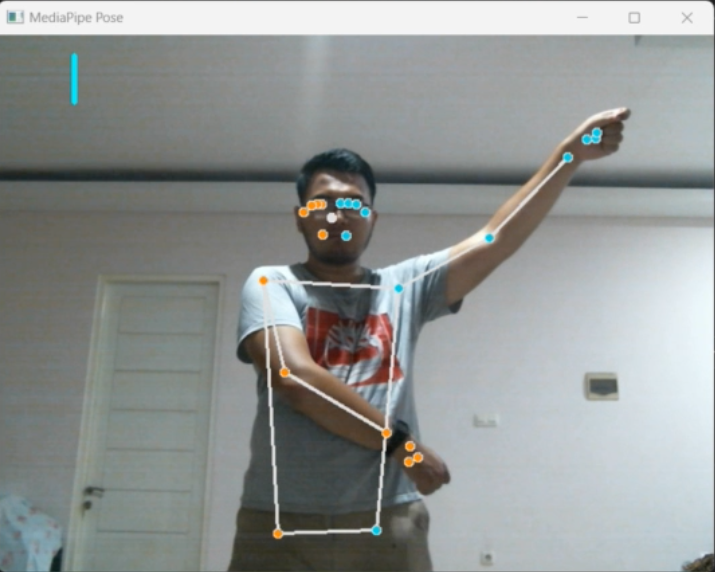
\includegraphics[width=0.2\textwidth]{gambar/bener/HurufI_ModelCNNResNet50V2_Dawe.png} \\
	\hline
	3 & U & 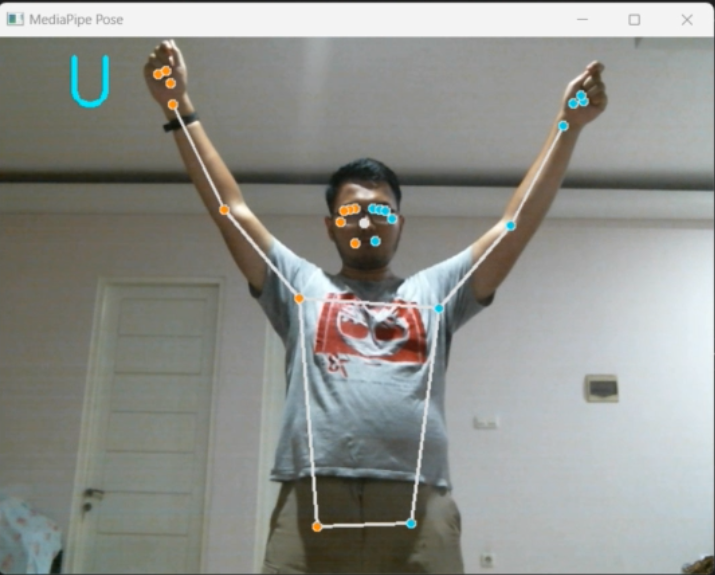
\includegraphics[width=0.2\textwidth]{gambar/bener/HurufU_ModelCNNResNet50V2_Dawe.png} \\
	\hline
	4 & E & 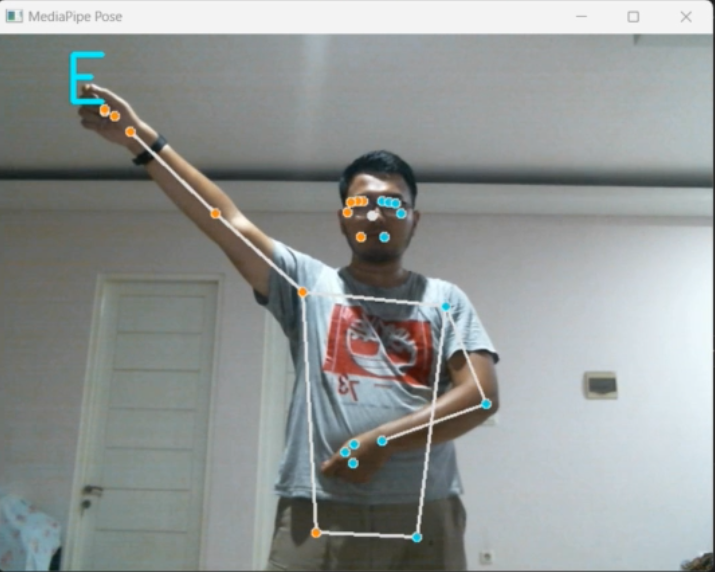
\includegraphics[width=0.2\textwidth]{gambar/bener/HurufE_ModelCNNResNet50V2_Dawe.png} \\
	\hline
	5 & O & \includegraphics[width=0.2\textwidth]{gambar/bener/HurufO_ModelCNNResNet50V2_Dawe.png} \\
	\hline
	6 & B & \includegraphics[width=0.2\textwidth]{gambar/bener/HurufB_ModelCNNResNet50V2_Dawe.png} \\
	\hline
	7 & K & \includegraphics[width=0.2\textwidth]{gambar/bener/HurufK_ModelCNNResNet50V2_Dawe.png} \\
	\hline
	8 & H & \includegraphics[width=0.2\textwidth]{gambar/bener/HurufH_ModelCNNResNet50V2_Dawe.png} \\
	\hline
	% Lanjutkan baris tabel sesuai kebutuhan
	\end{tabular}
\end{table}


\subsubsection*{Hasil Model CNN \textit{Xception} Orang Pertama}
Berdasarkan eksperimen yang dilakukan, ModelCNN \textit{Xception} telah berhasil dalam melakukan deteksi huruf dengan tingkat keberhasilan yang tinggi. Salah satu keunggulan utama dari model ini adalah kemampuannya dalam mengenali huruf dengan akurasi yang baik, bahkan ketika huruf tersebut berada dalam pose yang berbeda. Ujicoba tersebut telah menunjukkan bahwa ModelCNN \textit{Xception} mampu mengatasi tantangan yang mungkin muncul akibat variasi pose huruf, sehingga memberikan hasil yang akurat dalam pengenalan huruf

\begin{table}[!hbt]
	\centering
	\captionof{table}{Tabel Contoh Huruf/Kata dan Gambar Pose Model CNN Xception Orang Pertama}
	\label{tbl:Tabel Contoh Huruf/Kata dan Gambar Pose Model CNN Xception Orang Pertama}
	\begin{tabular}{|c|c|c|}
	\hline
	No & Huruf/Kata & Gambar Pose Model  \\
	\hline
	1 & A & \includegraphics[width=0.2\textwidth]{gambar/bener/HurufA_ModelCNNXception_Dawe.png} \\
	\hline
	2 & I & \includegraphics[width=0.2\textwidth]{gambar/bener/HurufI_ModelCNNXception_Dawe.png} \\
	\hline
	3 & U & \includegraphics[width=0.2\textwidth]{gambar/bener/HurufU_ModelCNNXception_Dawe.png} \\
	\hline
	4 & E & \includegraphics[width=0.2\textwidth]{gambar/bener/HurufE_ModelCNNXception_Dawe.png} \\
	\hline
	5 & O & \includegraphics[width=0.2\textwidth]{gambar/bener/HurufO_ModelCNNXception_Dawe.png} \\
	\hline
	6 & B & \includegraphics[width=0.2\textwidth]{gambar/bener/HurufB_ModelCNNXception_Dawe.png} \\
	\hline
	7 & K & \includegraphics[width=0.2\textwidth]{gambar/bener/HurufK_ModelCNNXception_Dawe.png} \\
	\hline
	8 & H & \includegraphics[width=0.2\textwidth]{gambar/bener/HurufH_ModelCNNXception_Dawe.png} \\
	\hline
	% Lanjutkan baris tabel sesuai kebutuhan
	\end{tabular}
\end{table}


\subsection{Orang Kedua}

Dalam serangkaian ujicoba ini, dilakukan pengujian terhadap seorang subjek kedua menggunakan beberapa model CNN yang berbeda, seperti Model CNN, Model CNN2, Model CNN ResNet50V2, dan Model CNN Xception. Ujicoba ini dilakukan dengan tujuan untuk mengevaluasi kemampuan masing-masing model dalam mengenali huruf dan membentuk kata.

Subjek kedua menjadi partisipan yang diuji dalam setiap percobaan menggunakan model-model tersebut. Melalui ujicoba ini, diharapkan dapat diperoleh pemahaman yang lebih mendalam mengenai keefektifan dan keandalan setiap model dalam pengenalan huruf dan pembentukan kata-kata

\subsubsection*{Hasil Model CNN Orang Kedua}

Berdasarkan percobaan yang dilakukan, ModelCNN telah menunjukkan kemampuannya yang baik dalam mengenali dan mendeteksi huruf dengan akurasi yang memuaskan.

\begin{table}[!hbt]
	\centering
	\captionof{table}{Tabel Contoh Huruf/Kata dan Gambar Pose Model CNN}
	\label{tbl:Tabel Contoh Huruf/Kata dan Gambar Pose Model CNN Orang Kedua}
	\begin{tabular}{|c|c|c|}
	\hline
	No & Huruf/Kata & Gambar Pose Model CNN \\
	\hline
	1 & A & \includegraphics[width=0.2\textwidth]{gambar/bener/HurufA_ModelCNN_Fachry.png} \\
	\hline
	2 & I & \includegraphics[width=0.2\textwidth]{gambar/bener/HurufI_ModelCNN_Fachry.png} \\
	\hline
	3 & U & \includegraphics[width=0.2\textwidth]{gambar/bener/HurufU_ModelCNN_Fachry.png} \\
	\hline
	4 & E & \includegraphics[width=0.2\textwidth]{gambar/bener/HurufE_ModelCNN_Fachry.png} \\
	\hline
	5 & O & \includegraphics[width=0.2\textwidth]{gambar/bener/HurufO_ModelCNN_Fachry.png} \\
	\hline
	6 & B & \includegraphics[width=0.2\textwidth]{gambar/bener/HurufB_ModelCNN_Fachry.png} \\
	\hline
	7 & K & \includegraphics[width=0.2\textwidth]{gambar/bener/HurufK_ModelCNN_Fachry.png} \\
	\hline
	8 & H & \includegraphics[width=0.2\textwidth]{gambar/bener/HurufH_ModelCNN_Fachry.png} \\
	\hline
	% Lanjutkan baris tabel sesuai kebutuhan
	\end{tabular}
	\end{table}

\begin{table}[!hbt]
	\centering
	\captionof{table}{Tabel Contoh Huruf/Kata dan Gambar Pose Model CNN2}
	\begin{tabular}{|c|c|c|}
		\hline
		No & Huruf/Kata & Gambar Pose Model  \\
		\hline
		9 & Bapak & \includegraphics[width=0.2\textwidth]{gambar/bener/HurufBapak_ModelCNN_Fachry.png} \\
		\hline
		10 & Ibu & \includegraphics[width=0.2\textwidth]{gambar/bener/HurufIbu_ModelCNN_Fachry.png} \\
		\hline
		11 & Tante & \includegraphics[width=0.2\textwidth]{gambar/bener/HurufTante_ModelCNN_Fachry.png} \\
		\hline
	\end{tabular}
\end{table}

\subsubsection*{Hasil Model CNN2 Orang Kedua}

Hasil ujicoba menunjukkan bahwa ModelCNN2 telah berhasil dalam melakukan deteksi huruf dengan tingkat keberhasilan yang baik.

\begin{table}[!hbt]
	\centering
	\captionof{table}{Tabel Contoh Huruf/Kata dan Gambar Pose Model CNN2 Orang Kedua}
	\label{tbl:Tabel Contoh Huruf/Kata dan Gambar Pose Model CNN2 Orang Kedua}
	\begin{tabular}{|c|c|c|}
	\hline
	No & Huruf/Kata & Gambar Pose Model  \\
	\hline
	1 & A & \includegraphics[width=0.2\textwidth]{gambar/bener/HurufA_ModelCNN2_Fachry.png} \\
	\hline
	2 & I & \includegraphics[width=0.2\textwidth]{gambar/bener/HurufI_ModelCNN2_Fachry.png} \\
	\hline
	3 & U & \includegraphics[width=0.2\textwidth]{gambar/bener/HurufU_ModelCNN2_Fachry.png} \\
	\hline
	4 & E & \includegraphics[width=0.2\textwidth]{gambar/bener/HurufE_ModelCNN2_Fachry.png} \\
	\hline
	5 & O & \includegraphics[width=0.2\textwidth]{gambar/bener/HurufO_ModelCNN2_Fachry.png} \\
	\hline
	6 & B & \includegraphics[width=0.2\textwidth]{gambar/bener/HurufB_ModelCNN2_Fachry.png} \\
	\hline
	7 & K & \includegraphics[width=0.2\textwidth]{gambar/bener/HurufK_ModelCNN2_Fachry.png} \\
	\hline
	8 & H & \includegraphics[width=0.2\textwidth]{gambar/bener/HurufH_ModelCNN2_Fachry.png} \\
	\hline
	% Lanjutkan baris tabel sesuai kebutuhan
	\end{tabular}
\end{table}

\begin{table}[!hbt]
	\centering
	\captionof{table}{Tabel Contoh Huruf/Kata dan Gambar Pose Model CNN2 Orang Kedua}
	\begin{tabular}{|c|c|c|}
		\hline
		No & Huruf/Kata & Gambar Pose Model  \\
		\hline
		9 & Bapak & \includegraphics[width=0.2\textwidth]{gambar/bener/HurufBapak_ModelCNN2_Fachry.png} \\
		\hline
		10 & Ibu & \includegraphics[width=0.2\textwidth]{gambar/bener/HurufIbu_ModelCNN2_Fachry.png} \\
		\hline
		11 & Tante & \includegraphics[width=0.2\textwidth]{gambar/bener/HurufTante_ModelCNN2_Fachry.png} \\
		\hline
	\end{tabular}
\end{table}

\subsubsection*{Hasil Model CNN \textit{ResNet50V2 }Orang Kedua}

Berdasarkan Hasil Ujicoba ,  ModelCNN \textit{ResNet50V2 }terkendala di deteksi huruf A , I , U , E , O , B , K dan H karena tidak mengeluarkan huruf sama sekali


\begin{table}[!hbt]
	\centering
	\captionof{table}{Tabel Contoh Huruf/Kata dan Gambar Pose Model CNN ResNet50V2 Orang Kedua}
	\label{tbl:Tabel Contoh Huruf/Kata dan Gambar Pose Model CNN ResNet50V2 Orang Kedua}
	\begin{tabular}{|c|c|c|}
	\hline
	No & Huruf/Kata & Gambar Pose Model  \\
	\hline
	1 & A & \includegraphics[width=0.2\textwidth]{gambar/bener/HurufA_ModelCNNResNet50V2_Fachry.png} \\
	\hline
	2 & I & \includegraphics[width=0.2\textwidth]{gambar/bener/HurufI_ModelCNNResNet50V2_Fachry.png} \\
	\hline
	3 & U & \includegraphics[width=0.2\textwidth]{gambar/bener/HurufU_ModelCNNResNet50V2_Fachry.png} \\
	\hline
	4 & E & \includegraphics[width=0.2\textwidth]{gambar/bener/HurufE_ModelCNNResNet50V2_Fachry.png} \\
	\hline
	5 & O & \includegraphics[width=0.2\textwidth]{gambar/bener/HurufO_ModelCNNResNet50V2_Fachry.png} \\
	\hline
	6 & B & \includegraphics[width=0.2\textwidth]{gambar/bener/HurufB_ModelCNNResNet50V2_Fachry.png} \\
	\hline
	7 & K & \includegraphics[width=0.2\textwidth]{gambar/bener/HurufK_ModelCNNResNet50V2_Fachry.png} \\
	\hline
	8 & H & \includegraphics[width=0.2\textwidth]{gambar/bener/HurufH_ModelCNNResNet50V2_Fachry.png} \\
	\hline
	% Lanjutkan baris tabel sesuai kebutuhan
	\end{tabular}
\end{table}


\subsubsection*{Hasil Model CNN \textit{Xception} Orang Kedua}

Berdasarkan Hasil Ujicoba  , ModelCNN \textit{Xception} sudah bisa melakukan deteksi dengan baik untuk huruf I , K , H , U dan E . Dan untuk huruf A masih meleset karena terbaca huruf G dan huruf O terbaca huruf D . Lalu untuk huruf B terbaca huruf H


\begin{table}[!hbt]
	\centering
	\captionof{table}{Tabel Contoh Huruf/Kata dan Gambar Pose Model CNN Xception Orang Kedua}
	\label{tbl:Tabel Contoh Huruf/Kata dan Gambar Pose Model CNN Xception Orang Kedua}
	\begin{tabular}{|c|c|c|}
	\hline
	No & Huruf/Kata & Gambar Pose Model  \\
	\hline
	1 & A & \includegraphics[width=0.2\textwidth]{gambar/bener/HurufA_ModelCNNXception_Fachry.png} \\
	\hline
	2 & I & \includegraphics[width=0.2\textwidth]{gambar/bener/HurufI_ModelCNNXception_Fachry.png} \\
	\hline
	3 & U & \includegraphics[width=0.2\textwidth]{gambar/bener/HurufU_ModelCNNXception_Fachry.png} \\
	\hline
	4 & E & \includegraphics[width=0.2\textwidth]{gambar/bener/HurufE_ModelCNNXception_Fachry.png} \\
	\hline
	5 & O & \includegraphics[width=0.2\textwidth]{gambar/bener/HurufO_ModelXception_Fachry.png} \\
	\hline
	6 & B & \includegraphics[width=0.2\textwidth]{gambar/bener/HurufB_ModelCNNXception_Fachry.png} \\
	\hline
	7 & K & \includegraphics[width=0.2\textwidth]{gambar/bener/HurufK_ModelCNNXception_Fachry.png} \\
	\hline
	8 & H & \includegraphics[width=0.2\textwidth]{gambar/bener/HurufH_ModelCNNXception_Fachry.png} \\
	\hline
	% Lanjutkan baris tabel sesuai kebutuhan
	\end{tabular}
\end{table}

  % Daftar pustaka
  \section{DAFTAR PUSTAKA}
  \renewcommand\refname{}
  \vspace{2ex}
  \renewcommand{\bibname}{
    @article
  }
  \begingroup
    \def\chapter*#1{}
    \printbibliography
  \endgroup


\end{document}
